\documentclass[
  babelLanguage=spanish,
  final,
  %showwirebinding,
  webversion,
  %showtrims,
]{chantingbook}

\usepackage{local}
\usepackage{graphicx}
\usepackage{subcaption}

\title{Libro de Cánticos}
\subtitle{Cánticos Matinales y Vespertinos (Pūjā) y Reflexiones}

% NOTE: This edition is subject to further editing. No ISBN for now.
%\ISBN{978-1-78432-031-7}

\editionInfo{\textit{Primera edición}, 2025}

\renewcommand\listfirstlinesname{Lista de Primeras Lineas}

\begin{document}

\frontmatter

\thispagestyle{empty}\mbox{}

% Not \webcover, b/c we're using \AddToShipoutPicture for cover design.
\ifwebversion
\mbox{}

\AddToShipoutPictureBG*{\put(0,0){%
\includegraphics[height=\paperheight]{vol1-webcover-bg.jpg}%
}}

\AddToShipoutPictureFG*{\put(\LenToUnit{30mm},\LenToUnit{85mm}){%
\begin{minipage}[b]{138mm}%
\raggedleft
\resizebox{100mm}{!}{\color[gray]{0}\Calluna Cânticos}
\end{minipage}%
}}

\AddToShipoutPictureFG*{\put(\LenToUnit{30mm},\LenToUnit{77mm}){%
\begin{minipage}[b]{138mm}%
\raggedleft
\fontsize{10.8}{10.8}\CallunaSans
\color[HTML]{DEB25D} VOLUME I
\hfill
\color[gray]{1} CÂNTICOS MATINAIS E VESPERTINOS (PŪJĀ) E REFLEXÕES
\end{minipage}%
}}

\AddToShipoutPictureFG*{\put(\LenToUnit{30mm},\LenToUnit{18mm}){%
\begin{minipage}[b]{138mm}%
\raggedleft
\fontsize{10.8}{10.8}\CallunaSans
PĀLI\hspace*{8pt}|\hspace*{8pt}PORTUGUÊS
\end{minipage}%
}}

%{\centering
%\mbox{}
%\vfill
%
%\parttitlefont\color{chaptertitle}
%%\addfontfeature{LetterSpace=2.0}
%
%Livro de Cânticos
%
%\vspace*{4\baselineskip}
%
%\vfill
%
%\mbox{}
%}
%
\fi

\clearpage

\cleartoverso

\thispagestyle{empty}

\enlargethispage{\baselineskip}

{\centering\small
\setlength{\parskip}{15pt}

{\normalsize
\thetitle\\
\thesubtitle\\
Pāli e Português}

Publicações Sumedhārāma\\
\href{http://sumedharama.pt}{www.sumedharama.pt}

Para distribuição gratuita\\
\textit{Sabbadānaṁ dhammadānaṁ jināti}\\
‘A oferta de Dhamma é superior a qualquer outra oferta.’

Este livro encontra-se disponível para distribuição gratuita em\\
\href{http://sumedharama.pt}{www.sumedharama.pt}

% ISBN \theISBN

Copyright \copyright\ Publicações Sumedhārāma 2024

Editores: Ajahn Amaro, Ajahn Gavesako\\
Tradutores: Ajahn Dhammiko, Ajahn Appamādo\\
Formatação: Ajahn Gambhīro\\
Capa: Nicholas Halliday

\vfill

Este trabalho está licenciado com uma Licença Creative Commons\\
Atribuição-NãoComercial-SemDerivações 4.0 Internacional.

Veja página \pageref{copyright-details} para mais detalhes sobre direitos e restrições desta licença.

Produzido com o sistema tipográfico \LaTeX.\\
Fonte utilizada: Gentium Incantation, Alegreya Sans e Ubuntu.

\theEditionInfo

}


\cleartorecto
\tableofcontents*

\clearpage
\chapterstyle{tocchapternoskip}
\listfirstlines*


\mainmatter


% ===
\morningPartSettings

\part{Cánticos Matinales}

\morningChapterSettings

\chapter{Dedicación de Ofrendas}

[Yo so] bha꜕gavā a꜕rahaṁ sammāsambuddho

\begin{english}
Al Excelso, el Maestro, que totalmente alcanzó la iluminación perfecta,
\end{english}

Svākkhā꜓to yena bha꜕gava꜓tā dhammo

\begin{english}
A las enseñanzas, tan bien explicadas por Él,
\end{english}

Supaṭi꜕panno yassa bha꜕gava꜕to sāvaka꜕saṅgho

\begin{english}
A los discípulos del Maestro, que tan bien practicaron,
\end{english}

Tam-ma꜓yaṁ bha꜕gavantaṁ sa꜕dhammaṁ sa꜕saṅghaṁ

\begin{english}
A estos – al Buddha, al Dhamma y a la Saṅgha ---
\end{english}

Imehi꜓ sakkārehi꜕ yathārahaṁ āropi꜕tehi a꜕bhi꜓pūja꜕yāma

\begin{english}
Presentamos el debido homenaje con ofrendas.
\end{english}

Sādhu꜓ no bhante bha꜕gavā su꜕cira-parinibbu꜕topi

\begin{english}
Es excelente para nosotros que el Excelso, habiéndose liberado
\end{english}

Pacchi꜓mā-ja꜕na꜓tānu꜓kampa꜕-mānasā

\begin{english}
Haya tenido compasión por las generaciones futuras.
\end{english}

Ime sakkāre dugga꜕ta꜕-paṇṇākāra꜓-bhūte pa꜕ṭiggaṇhātu

\begin{english}
Que estas simples ofrendas sean aceptadas
\end{english}

Amhā꜓kaṁ dīgha꜕rattaṁ hi꜕tāya su꜕khāya

\begin{english}
Por nuestro beneficio duradero y por la felicidad que nos da.
\end{english}

\clearpage

Arahaṁ sammāsambuddho bha꜕gavā

\begin{english}
Al Maestro, el perfectamente Iluminado y Excelso
\end{english}

Buddhaṁ bha꜕gavantaṁ a꜕bhi꜓vādemi

\begin{english}
  Al Buddha, el Excelso, yo rindo homenaje.
  \instr{Reverencia}
\end{english}

[Svākkhā꜓to] bha꜕gava꜓tā dhammo

\begin{english}
 A las enseñanzas, tan bien explicadas por Él 
\end{english}

Dhammaṁ namassāmi

\begin{english}
  Al Dhamma, yo rindo homenaje.
  \instr{Reverencia}
\end{english}

[Supaṭi꜕panno] bha꜕gava꜕to sāvaka꜕saṅgho

\begin{english}
A los discípulos del Maestro que tan bien practicaron
\end{english}

Sa꜓ṅghaṁ na꜕māmi

\begin{english}
  A la Saṅgha, yo rindo homenaje.
  \instr{Reverencia}
\end{english}

\chapter{Homenaje Preliminar}

\begin{leader}
  [Ha꜓nda mayaṁ buddhassa꜕ bha꜕gavato\\ pubbabhāga-namakā꜕raṁ karomase]
\end{leader}

\begin{english}
  [Rindamos ahora homenaje preliminar al Buddha]
\end{english}

\vspace{\baselineskip}

Namo tassa bha꜕gava꜕to araha꜕to sa꜓mmāsa꜓mbuddha꜕ssa

\instr{Tres veces}

\begin{english}
  Homenaje al Excelso, Noble y Perfectamente Iluminado.

  \instr{Tres veces}
\end{english}

\clearpage

\chapter{Homenaje al Buddha}

\begin{leader}
  [Ha꜓nda mayaṁ buddhābhi꜕tthu꜕tiṁ karomase]
\end{leader}

\begin{english}
  [Cantemos ahora en elogio al Buddha.]
\end{english}

Yo so tathā꜓ga꜕to a꜕rahaṁ sammāsambuddho

\begin{english}
  El Tathāgata es puro y perfectamente iluminado.
\end{english}

Vijjāca꜕raṇa꜓-sampanno

\begin{english}
  Impecable en conducta y comprensión,
\end{english}

Su꜕ga꜕to

\begin{english}
  Realizado,
\end{english}

Loka꜕vi꜓dū

\begin{english}
  Conocedor de los mundos.
\end{english}

Anu꜓tta꜕ro purisa꜕damma-sārathi

\begin{english}
  Él entrena perfectamente a aquellos que desean entrenarse.
\end{english}

Satthā deva-ma꜕nussānaṁ

\begin{english}
  Él es Maestro de dioses y humanos.
\end{english}

Buddho bha꜕gavā

\begin{english}
  Él es despierto y sagrado.
\end{english}

Yo imaṁ lokaṁ sa꜕devakaṁ sa꜕mārakaṁ sa꜕brahma꜕kaṁ

\begin{english}
  En este mundo \pause\ con sus dioses, demonios e espíritus gentiles,
\end{english}

Sassa꜓maṇa-brāhmaṇiṁ pa꜕jaṁ sa꜕deva-ma꜕nussa꜓ṁ sa꜕yaṁ a꜕bhiññā sacchika꜕tv꜓ā pa꜕vedesi

\begin{english}
  Sus buscadores y sabios, seres celestiales y humanos,\\ Él reveló la verdad a través de una comprensión profunda.
\end{english}

Yo dhammaṁ dese꜓si ā꜕di꜓-kalyāṇaṁ majjhe꜓-ka꜕lyāṇaṁ \\pa꜕riyosāna-k꜕alyāṇaṁ

\begin{english}
  Él explicó el Dhamma: Sublime al principio,\\ Sublime en el medio y Sublime al final.
\end{english}

Sāttha꜓ṁ sa꜕byañjanaṁ kevala-pa꜕ripuṇṇaṁ pa꜕risuddhaṁ \\brahma-ca꜕ri꜓yaṁ pa꜕kāsesi

\begin{english}
  Él explicó la vida espiritual de completa pureza,\\En su esencia y convenciones.
\end{english}

Tam-aha꜓ṁ bha꜕gavantaṁ a꜕bhi꜓pūja꜕yāmi tam-aha꜓ṁ bha꜕gavantaṁ \\si꜕rasā꜓ na꜕māmi

\begin{english}
  Yo canto mi elogio al Buddha, yo saludo respetuosamente \\al Excelso.
  \instr{Reverencia}
\end{english}

\clearpage

\chapter{Homenaje al Dhamma}

\begin{leader}
  [Ha꜓nda mayaṁ dhammābhi꜕tthu꜕tiṁ karomase]
\end{leader}

\begin{english}
  [Cantemos ahora en elogio al Dhamma]
\end{english}

Yo so svākkhā꜓to bha꜕gava꜓tā dhammo

\begin{english}
  El Dhamma, tan bien explicado por el Excelso,
\end{english}

Sa꜓ndiṭṭhi꜕ko

\begin{english}
  Presente aquí y ahora,
\end{english}

A꜕kāli꜕ko

\begin{english}
  Intemporal,
\end{english}

Ehi꜕passi꜕ko

\begin{english}
  Incentivando a investigar,
\end{english}

Opanayi꜕ko

\begin{english}
  Guiando al interior,
\end{english}

Pa꜕cca꜕ttaṁ vedi꜓ta꜕bbo viññūhi

\begin{english}
  Para ser experimentado individualmente por los sabios.
\end{english}

Tam-aha꜓ṁ dhammaṁ a꜕bhi꜓pūja꜕yāmi tam-aha꜓ṁ dhammaṁ \\si꜕rasā꜓ na꜕māmi

\begin{english}
  Yo canto mi elogio a estas enseñanzas,\\
  yo saludo respetuosamente esta verdad.
  \instr{Reverencia}
\end{english}

\clearpage

\chapter{Homenaje a la Saṅgha}

\begin{leader}
  [Ha꜓nda mayaṁ saṅghābhi꜕tthu꜕tiṁ karomase]
\end{leader}

\begin{english}
  [Cantemos ahora en elogio a la Saṅgha.]
\end{english}

Yo so supaṭi꜕panno bha꜕gava꜕to sāvaka꜕saṅgho

\begin{english}
  Son los discípulos del Maestro que practicaron correctamente,
\end{english}

Ujupaṭi꜕panno bha꜕gava꜕to sāvaka꜕saṅgho

\begin{english}
  Que practicaron directamente,
\end{english}

Ñāyapaṭi꜕panno bha꜕gava꜕to sāvaka꜕saṅgho

\begin{english}
  Que practicaron con reflexión,
\end{english}

Sā꜓mīci꜕pa꜕ṭi꜕panno bha꜕gava꜕to sāvaka꜕saṅgho

\begin{english}
  Aquellos que practicaron con integridad ---
\end{english}

Yadidaṁ cattāri purisa꜕yugāni aṭṭha꜓ purisa꜕pugga꜕lā

\begin{english}
  Es decir, los cuatro pares, los ocho tipos de Seres Nobles ---
\end{english}

Esa bha꜕gava꜕to sāvaka꜕saṅgho

\begin{english}
 Estos son los discípulos del Maestro.
\end{english}

Āhu꜕neyyo

\begin{english}
  Tales discípulos son merecedores de presentes,
\end{english}

Pāhu꜕neyyo

\begin{english}
  Merecedores de hospitalidad,
\end{english}

\clearpage

Dakkhi꜕ṇeyyo

\begin{english}
  Merecedores de ofrendas,
\end{english}

Añja꜕li-ka꜕ra꜓ṇīyo

\begin{english}
  Merecedores de respeto;
\end{english}

Anu꜓tta꜕raṁ puññakkhe꜕ttaṁ lokassa

\begin{english}
  Ellos promueven el surgir \pause\ de un bien incomparable\\ en el mundo.
\end{english}

Tam-aha꜓ṁ saṅghaṁ a꜕bhi꜓pūja꜕yāmi tam-aha꜓ṁ saṅghaṁ\\ si꜕rasā꜓ na꜕māmi

\begin{english}
  Yo canto mi elogio a esta Saṅgha,\\
  yo saludo respetuosamente a esta Saṅgha.
  \instr{Reverencia}
\end{english}

\clearpage

\chapter{Saludo a la Joya Triple}

\begin{leader}
  [Ha꜓nda mayaṁ ratanattaya-paṇāma-gāthā꜓yo c'eva\\
  sa꜓ṁvega-parikittana-pāṭhañca꜕ bhaṇāmase]
\end{leader}

\begin{english}
  [Cantemos ahora nuestro saludo a la Joya Triple \pause\ y los versos\\ que estimulan el sentido de urgencia.]
\end{english}

Buddho su꜕suddho ka꜕ruṇā-maha꜓ṇṇavo

\begin{english}
  El Buddha \pause\ absolutamente puro, con compasión como el Océano,
\end{english}

Yo'ccanta꜕-suddhabba꜕ra-ñāṇa꜕-loca꜕no

\begin{english}
 Poseyendo la visión clara de Sabiduría,
\end{english}

Lokassa꜕ pāpūpa꜕ki꜓lesa꜕-ghāta꜕ko

\begin{english}
  Destructor de los defectos mundanos 
\end{english}

Vandāmi꜓ buddhaṁ a꜕ha꜓m-āda꜕rena꜕ taṁ

\begin{english}
  En plena devoción, ese Buddha yo venero.
\end{english}

Dhammo pa꜕dīpo vi꜕ya tassa꜕ satthu꜕no

\begin{english}
  Las enseñanzas del Maestro, como una lámpara,
\end{english}

Yo magga꜓-pākāma꜕ta꜕-bheda꜕-bhinna꜕ko

\begin{english}
  Iluminan el camino y su fruto: la Realidad Inmortal,
\end{english}

Lokuttaro yo ca꜕ ta꜕d-attha꜕-dīpa꜕no

\begin{english}
  Aquello que está más allá del mundo condicionado 
\end{english}

Vandāmi꜓ dhammaṁ a꜕ha꜓m-āda꜕rena꜕ taṁ

\begin{english}
  En plena devoción, ese Dhamma yo venero.
\end{english}

Sa꜓ṅgho su꜕khettābhyati-khe꜕tta-sa꜓ññito

\begin{english}
  La Saṅgha, el mejor terreno para el cultivo,
\end{english}

Yo diṭṭha꜓-santo su꜕ga꜕tānu꜕bodha꜕ko

\begin{english}
  Aquellos que realizaron la paz, despertando después del Maestro,
\end{english}

Lolappa꜕hīno a꜕ri꜓yo su꜕medha꜕so

\begin{english}
  Nobles y Sabios, habiendo abandonado todo anhelo, 
\end{english}

Vandāmi꜓ saṅghaṁ a꜕ha꜓m-āda꜕rena꜕ taṁ

\begin{english}
 En plena devoción, esa Saṅgha yo venero.
\end{english}

Iccevam-ekanta꜕bhi꜓pūja꜕-neyya꜕kaṁ vatthuttayaṁ \\vanda꜕ya꜕tābhi꜕saṅkha꜕taṁ

\begin{english}
 Este saludo debe ser hecho \pause\ a lo que tiene valor.
\end{english}

Puññaṁ ma꜕yā yaṁ ma꜕ma꜕ sabbu꜕padda꜕vā mā ho꜓ntu꜕ ve tassa꜕ pa꜕bhāva꜕-siddhi꜕yā

\begin{english}
  A través del poder de esta acción benéfica, que todos los obstáculos puedan ser vencidos.
\end{english}

Idha tathā꜓ga꜕to loke u꜕ppanno a꜕rahaṁ sammāsambuddho

\begin{english}
  Aquel que conoce las cosas como son, vino a este mundo y es un Arahant, un ser perfectamente despierto.
\end{english}

Dhammo ca꜕ desi꜕to niyyāni꜕ko u꜕pa꜕sa꜕miko pa꜕rinibbāni꜕ko sa꜓mbodha꜕gāmī su꜕ga꜕tappa꜕vedi꜕to

\enlargethispage{\baselineskip}

\begin{english}
  Purificando la vía que libera de la ilusión, tranquilizando y dirigiéndose hacia la paz perfecta, guiando a la Iluminación: Este Camino Él dió a conocer.
\end{english}

Ma꜓yan-taṁ dhammaṁ su꜕tvā evaṁ jānāma

\begin{english}
  Habiendo oído las Enseñanzas sabemos lo siguiente:
\end{english}

Jātipi꜕ dukkhā

\begin{english}
  El nacimiento es dukkha,
\end{english}

Jarāpi꜕ dukkhā

\begin{english}
  El envejecimiento es dukkha,
\end{english}

Ma꜕raṇampi꜕ dukkhaṁ

\begin{english}
  La muerte es dukkha;
\end{english}

So꜓ka-pa꜕rideva-dukkha꜕-domanass'u꜕pāyāsā꜓pi꜕ dukkhā

\begin{english}
  Tristeza, lamentación, dolor, angustia y desespero son dukkha;
\end{english}

Appiyehi꜕ sa꜓mpa꜕yogo dukkho

\begin{english}
  Asociación con lo que no gusta es dukkha;
\end{english}

Piyehi꜕ vi꜓ppa꜕yogo dukkho

\begin{english}
  Separación de lo que gusta es dukkha;
\end{english}

Yamp'iccha꜓ṁ na꜕ labhati tampi꜕ dukkhaṁ

\begin{english}
  No alcanzar aquello que se quiere es dukkha.
\end{english}

Sa꜓ṅkhittena pañcu꜕pādānakkha꜓ndhā dukkhā

\begin{english}
  Resumiendo, las cinco khandhas son dukkha.
\end{english}

Seyya꜕thīdaṁ

\begin{english}
  Estas son:
\end{english}

\clearpage

Rūpūpādāna꜕kkha꜓ndho

\begin{english}
  Apego a la forma,
\end{english}

Vedanūpādāna꜕kkha꜓ndho

\begin{english}
  Apego a la sensación,
\end{english}

Sa꜓ññūpādāna꜕kkha꜓ndho

\begin{english}
  Apego a la percepción,
\end{english}

Sa꜓ṅkhā꜓rūpādāna꜕kkha꜓ndho

\begin{english}
  Apego a las formaciones mentales,
\end{english}

Viññāṇūpādāna꜕kkha꜓ndho

\begin{english}
  Apego a la cognición.
\end{english}

Yesaṁ pa꜕riññāya

\begin{english}
  Para esta total comprensión,
\end{english}

Dha꜕ramāno so꜓ bha꜕gavā evaṁ ba꜕hulaṁ sā꜓va꜕ke vi꜕neti

\begin{english}
  Durante su vida, el Excelso instruyó frecuentemente así a sus\\ discípulos.
\end{english}

Evaṁ bhāgā ca꜕ panassa bha꜕gava꜕to sā꜓va꜕kesu a꜕nusā꜓sa꜕nī ba꜕hulā pa꜕vatta꜕ti

\begin{english}
  Más allá de eso, Él instruyó:
\end{english}


Rūpaṁ a꜕niccaṁ

\begin{english}
  La forma no es permanente,
\end{english}

Vedanā a꜕niccā

\begin{english}
  La sensación no es permanente,
\end{english}

Sa꜓ññā a꜕niccā

\begin{english}
  La percepción no es permanente,
\end{english}

Sa꜓ṅkhā꜓rā a꜕niccā

\begin{english}
  Las formaciones mentales no son permanentes,
\end{english}

Viññāṇaṁ a꜕niccaṁ

\begin{english}
  La cognición no es permanente;
\end{english}

Rūpaṁ a꜕nattā

\begin{english}
  La forma no es 'yo',
\end{english}

Vedanā a꜕nattā

\begin{english}
  La sensación no es 'yo',
\end{english}

Sa꜓ññā a꜕nattā

\begin{english}
  La percepción no es 'yo',
\end{english}

Sa꜓ṅkhā꜓rā a꜕nattā

\begin{english}
  Las formaciones mentales no son 'yo',
\end{english}

Viññāṇaṁ a꜕nattā

\begin{english}
  La cognición no es 'yo';
\end{english}

Sa꜕bbe sa꜓ṅkhā꜓rā a꜕niccā

\begin{english}
  Ninguna condicion es permanente,
\end{english}

Sa꜕bbe dhammā a꜕nattā'ti

\begin{english}
  No hay un 'yo' en lo creado o lo increado.
\end{english}

\clearpage

Te ma꜓yaṁ otiṇṇāmha jāti꜕yā ja꜕rā-maraṇena

\begin{english}
  Todos nosotros nos vemos arrastrados por el nacimiento, el envejecimiento y la muerte,
\end{english}

So꜓kehi꜕ pa꜕ridevehi꜕ dukkhe꜓hi꜕ domanassehi꜕ u꜕pāyāsehi

\begin{english}
  Por la tristeza, lamentación, dolor, angustia y desespero,
\end{english}

Dukkho꜓tiṇṇā dukkha꜕-pa꜕retā

\begin{english}
  Arrastrados por dukkha y obstruidos por dukkha.
\end{english}

Appeva nāmi꜓massa꜕ kevalassa꜕ dukkha-kkha꜓ndhassa꜕ anta꜕kiri꜓yā \\paññāyethā'ti

\begin{english}
  Que alcancemos el fin de toda esta masa de sufrimiento.
\end{english}

\begin{instruction}
  La parte que sigue es cantada solamente por los monjes.
\end{instruction}

Ci꜓ra꜓-pari꜕nibbutampi꜓ taṁ bha꜕gava꜓ntaṁ uddissa a꜕raha꜓ntaṁ sammāsambuddhaṁ

\begin{english}
  Recordando al Excelso, el Noble Maestro, el Perfectamente Iluminado, que hace mucho alcanzó el Parinibbāna,
\end{english}

Saddhā a꜕gārasmā anagāri꜓yaṁ pabba꜕ji꜕tā

\begin{english}
  Partimos con confianza del hogar hacia la vida monástica.
\end{english}

Tasmi꜓ṁ bha꜕gavati brahma-ca꜕ri꜓yaṁ ca꜕rāma

\begin{english}
  Así como el Iluminado, practicamos la Vida Sagrada,
\end{english}

Bhikkhū꜓naṁ si꜓kkhāsā꜕jīva꜕-samāpannā

\begin{english}
  Completamente equipados con el sistema de entrenamiento de los Bhikkhus.
\end{english}

\clearpage

Taṁ no brahma-ca꜕ri꜓yaṁ imassa꜕ kevalassa꜕ dukkha-kkha꜓ndhassa꜕ anta꜕kiri꜓yāya sa꜓ṁva꜓tta꜕tu

\begin{english}
  Que esta vida purificada \pause\ pueda conducirnos \pause\ al término de toda esta masa de sufrimiento.
\end{english}

\begin{instruction}
  Una versión alternativa de la sección anterior, que puede ser también cantada por los laicos.
\end{instruction}

Ci꜓ra꜓-pari꜕nibbutampi꜓ taṁ bha꜕gava꜓ntaṁ saraṇaṁ ga꜕tā

\begin{english}
  El Excelso, aunque hace tiempo alcanzó el Parinibbāna, es nuestro refugio.
\end{english}

Dha꜓mmañca sa꜓ṅghañca

\begin{english}
  Así como el Dhamma y la Saṅgha.
\end{english}

Tassa bha꜕gavato sā꜓sanaṁ yathā꜓-sati yathā꜓-balaṁ manasika꜕roma a꜕nupaṭipa꜓jjāma

\begin{english}
  Seguimos el camino de aquel Excelso, atentamente con toda\\ nuestra fuerza y conciencia.
\end{english}

Sā꜓ sā꜓ no pa꜕ṭi꜓patti

\begin{english}
  Que el cultivo de esta práctica
\end{english}

Imassa꜕ kevalassa꜕ dukkha-kkha꜓ndhassa꜕ anta꜕kiri꜓yāya sa꜓ṁva꜓tta꜕tu

\begin{english}
 Pueda conducirnos  \pause\  al término de toda esta masa de sufrimiento.
\end{english}

\clearpage

\chapter{Homenaje de Cierre}

[Arahaṁ] sammāsambuddho bha꜕gavā

\begin{english}
  Al Maestro, el perfectamente Iluminado y Excelso 
\end{english}

Buddhaṁ bha꜕gavantaṁ a꜕bhi꜓vādemi

\begin{english}
  Al Buddha, el Excelso, yo rindo homenaje.
  \instr{Reverencia}
\end{english}

[Svākkhā꜓to] bha꜕gava꜓tā dhammo

\begin{english}
  A las Enseñanzas, tan bien explicadas por Él 
\end{english}

Dhammaṁ namassāmi

\begin{english}
  Al Dhamma, yo rindo homenaje.
  \instr{Reverencia}
\end{english}


[Supaṭi꜕panno] bha꜕gava꜕to sāvaka꜕saṅgho

\begin{english}
  A los discípulos del Excelso que tan bien practicaron
\end{english}

Sa꜓ṅghaṁ na꜕māmi

\begin{english}
  A la Saṅgha, yo rindo homenaje.
  \instr{Reverencia}
\end{english}


\morningSettingsRestore

% ===
\eveningPartSettings

\part{Cánticos Vespertinos}

\eveningChapterSettings

\chapter*{Dedicación de Ofrendas}

\delegateSetUseNext

[Yo so] bha꜕gavā a꜕rahaṁ sammāsambuddho\\
Svākkhā꜓to yena bha꜕gava꜓tā dhammo\\
Supaṭi꜕panno yassa bha꜕gava꜕to sāvaka꜕saṅgho\\
Tam-ma꜓yaṁ bha꜕gavantaṁ sa꜕dhammaṁ sa꜕saṅghaṁ\\
Imehi꜓ sakkārehi꜕ yathārahaṁ āropi꜕tehi a꜕bhi꜓pūja꜕yāma\\
Sādhu꜓ no bhante bha꜕gavā su꜕cira-parinibbu꜕topi\\
Pacchi꜓mā-ja꜕na꜓tānu꜓kampa꜕-mānasā\\
Ime sakkāre dugga꜕ta꜕-paṇṇākāra꜓-bhūte pa꜕ṭiggaṇhātu\\
Amhā꜓kaṁ dīgha꜕rattaṁ hi꜕tāya su꜕khāya

Arahaṁ sammāsambuddho bha꜕gavā\\
Buddhaṁ bha꜕gavantaṁ a꜕bhi꜓vādemi \instr{Reverencia}

[Svākkhā꜓to] bha꜕gava꜓tā dhammo\\
Dhammaṁ namassāmi \instr{Reverencia}

[Supaṭi꜕panno] bha꜕gava꜕to sāvaka꜕saṅgho\\
Sa꜓ṅghaṁ na꜕māmi \instr{Reverencia}

\clearpage

\chapter{Dedicación de Ofrendas}

[Al Iluminado,] el Maestro, que totalmente alcanzó\\
\vin la iluminación perfecta,\\
A las enseñanzas, tan bien explicadas por Él,\\
A los discípulos del Maestro, que tan bien practicaron,\\
A estos – al Buddha, al Dhamma y a la Saṅgha ---\\
Presentamos el debido homenaje con ofrendas.\\
Es excelente para nosotros que el Excelso, habiéndose liberado,\\
Haya tenido compasión por las generaciones futuras.\\
Que estas simples ofrendas sean aceptadas\\
Para nuestro duradero beneficio y por la felicidad que nos da.
 
 
\bigskip


Al Maestro, el perfectamente Iluminado y Excelso ---\\
Al Buddha, el Excelso, yo rindo homenaje. \instr{Reverencia}

\bigskip

[A las enseñanzas,] tan bien explicadas por Él ---\\
Al Dhamma, yo rindo homenaje. \instr{Reverencia}

\bigskip

[A los discípulos del Maestro,] que tan bien practicaron\\
A la Saṅgha, yo rindo homenaje. \instr{Reverencia}

\clearpage

\chapter*{Homenaje Preliminar}

\begin{leader}
  [Ha꜓nda mayaṁ buddhassa꜕ bhagavato\\ pubbabhāga-namakā꜕raṁ karomase]
\end{leader}

Namo tassa bha꜕gava꜕to araha꜕to sa꜓mmāsa꜓mbuddha꜕ssa

\instr{Tres veces}

\chapter*{Remembranza del Buddha}

\delegateSetUseNext

\begin{leader}
  [Ha꜓nda mayaṁ buddhānu꜕ssa꜕ti꜕nayaṁ karomase]
\end{leader}

Taṁ kho꜓ pana bha꜕gavantaṁ evaṁ kaly꜓āṇo kitti꜕saddo abbhugga꜕to\\
Itipi so bha꜕gavā a꜕rahaṁ sammāsambuddho\\
Vijjāca꜕raṇa꜓-sampanno su꜕ga꜕to loka꜕vi꜓dū\\
Anu꜓tta꜕ro purisa꜕damma-sārathi satthā deva-ma꜕nussānaṁ\\
\vin buddho bha꜕gavā'ti

\clearpage

\chapter{Homenaje Preliminar}

\begin{leader}
  [Rindamos ahora homenaje preliminar al Buddha.]
\end{leader}

Homenaje al Excelso, Noble y Perfectamente Iluminado.

\instr{Tres veces}

\nextChapterUseDelegatedPageNumber

\chapter{Remembranza del Buddha}

\begin{leader}
  [Cantemos ahora la remembranza del Buddha.]
\end{leader}

Con la buena nueva sobre la reputación del Excelso,\\
\vin se ha oído lo siguiente:\\
Él, el Excelso, es realmente el Puro,\\
\vin el Perfectamente Iluminado;\\
Él es Impecable en conducta y comprensión,\\
\vin el Realizado, el Conocedor de los Mundos;\\
Él adiestra perfectamente aquellos que desean ser adiestrados;\\
Él es Maestro de dioses y humanos;\\
Él es Despierto y Sagrado.

\clearpage

\chapter*{Elogio Supremo al Buddha}

\delegateSetUseNext

\begin{leader}
  [Ha꜓nda mayaṁ buddhābhi꜕gī꜕tiṁ karomase]
\end{leader}

Buddh'vāra꜕ha꜓nta-varatādi꜕gu꜓ṇābhi꜕yutto\\
Suddhābhi꜕ñāṇa-ka꜕ru꜓ṇāhi sa꜓māga꜕tatto\\
Bodhesi꜕ yo su꜕ja꜕na꜓taṁ ka꜕ma꜓laṁ va꜕ sūro\\
Vandām'aha꜓ṁ ta꜕m-ara꜕ṇaṁ si꜕rasā꜓ ji꜕nendaṁ\\
Buddho yo sabba꜕-pāṇīnaṁ sa꜕raṇaṁ khema꜕m-utta꜕maṁ\\
Pa꜕ṭhamānussa꜕tiṭṭhānaṁ vandāmi꜕ taṁ si꜓ren'a꜕haṁ\\
Buddhassā꜓h'a꜕smi dāso/dāsī va buddho me sā꜕mi-ki꜓ssaro\\
Buddho dukkhassa꜕ ghātā ca꜕ vidhātā ca꜕ hi꜓tassa꜕ me\\
Buddhass'āha꜓ṁ niyyādemi sa꜕rīrañ-jīvi꜕tañ-ci꜕daṁ\\
Vandanto'ha꜓ṁ/Vandantī'ha꜓ṁ ca꜕rissāmi buddhass'eva꜕ su꜓bodhi꜕taṁ\\
Natthi me sa꜕ra꜓ṇaṁ aññaṁ buddho me sa꜕ra꜓ṇaṁ va꜕raṁ\\
Etena sacca꜕-vajjena vaḍḍheyyaṁ sa꜕tthu-sā꜓sane\\
Buddhaṁ me vanda꜕mānena/vanda꜕mānāya\\
\vin yaṁ puññaṁ pa꜕su꜓taṁ i꜕dha\\
Sa꜕bbepi anta꜕rāyā me māhe꜓su꜓ṁ ta꜕ssa꜓ teja꜕sā

\begin{instruction}
  Reverencia
\end{instruction}

Kāyena vācāya va ceta꜕sā꜓ vā\\
Bu꜓ddhe ku꜕kammaṁ pa꜕kataṁ ma꜕yā yaṁ\\
Bu꜓ddho pa꜕ṭiggaṇhā꜕tu acca꜕yantaṁ\\
Kālantare sa꜓ṁvarituṁ va꜕ bu꜓ddhe

\clearpage

\chapter{Elogio Supremo al Buddha}

\begin{leader}
  [Cantemos ahora en elogio supremo al Buddha.]
\end{leader}

El Buddha, verdaderamente valorable,\\
\vin dotado de tan excelentes cualidades,\\
Cuyo ser está compuesto de pureza,\\
\vin sabiduría transcendental y compasión,\\
Que iluminó a los sabios, así como el sol despierta la flor del loto ---\\
Yo venero ese pacífico líder de conquistadores.\\
El Buddha, que es el refugio seguro y supremo de todos los seres ---\\
Como primer objeto de remembranza, yo lo venero postrándome.\\
Soy de hecho el sirviente de Buddha, Buddha es mi maestro y guía.\\
Buddha es el destructor de tristeza, que proyecta bendiciones sobre mí.\\
A Buddha, me dedico en cuerpo y alma,\\
Y en devoción caminaré, el Sendero del Despertar de Buddha.\\
Para mí no existe otro refugio, Buddha es mi excelente refugio.\\
Por la afirmación de esta Verdad,\\
\vin que yo crezca en el camino del Maestro.\\
Por mi devoción a Buddha, y por el mérito de esta práctica ---\\
Por su poder, que todos los obstáculos sean vencidos.

\begin{instruction}
  Reverencia
\end{instruction}

De pensamiento, palabra u obra,\\
Por cualquier acción errónea que haya cometido hacia Buddha,\\
Que mi reconocimiento de esa falta sea aceptado,\\
De forma que en el futuro me refrene hacia Buddha.

\clearpage

\chapter*{Remembranza del Dhamma}

\delegateSetUseNext

\begin{leader}
  [Ha꜓nda mayaṁ dhammānu꜕ssa꜕ti꜕nayaṁ karomase]
\end{leader}

Svākkhā꜓to bha꜕gava꜓tā dhammo\\
Sa꜓ndiṭṭhi꜕ko a꜕kāli꜕ko ehi꜕passi꜕ko\\
Opanayi꜕ko pa꜕cca꜕ttaṁ vedi꜓ta꜕bbo viññūhī'ti

\chapter*{Elogio Supremo al Dhamma}

\begin{leader}
  [Ha꜓nda mayaṁ dhammābhi꜕gī꜕tiṁ karomase]
\end{leader}

Svākkhā꜓ta꜕t'ādi꜕guṇa-yoga꜕-va꜓sena꜕ seyyo\\
Yo magga꜕-pāka-pa꜕riyatti꜕-vi꜓mokkha꜕-bhedo\\
Dhammo ku꜕loka-pa꜕ta꜓nā ta꜕da꜓-dhāri꜕-dhārī\\
Vandām'aha꜓ṁ ta꜕ma-ha꜕raṁ va꜕ra-dha꜓mma꜕m-etaṁ\\
Dhammo yo sabba꜕-pāṇīnaṁ sa꜕raṇaṁ khema꜕m-utta꜕maṁ\\
Du꜕tiyānussa꜕tiṭṭhānaṁ vandāmi꜕ taṁ si꜓ren'a꜕haṁ\\
Dhammassā꜓h'a꜕smi dāso/dāsī va dhammo me sā꜕mi-ki꜓ssaro\\
Dhammo dukkhassa꜕ ghātā ca꜕ vidhātā ca꜕ hi꜓tassa꜕ me\\
Dhammass'āha꜓ṁ niyyādemi sa꜕rīrañ-jīvi꜕tañ-ci꜕daṁ\\
Vandantoha꜓ṁ/Vandantīha꜓ṁ ca꜕rissāmi dhammass'eva꜕ su꜓dhamma꜕taṁ\\
Natthi me sa꜕ra꜓ṇaṁ aññaṁ dhammo me sa꜕ra꜓ṇaṁ va꜕raṁ\\
Etena sacca꜕-vajjena vaḍḍheyyaṁ sa꜕tthu-sā꜓sane\\
Dhammaṁ me vanda꜕mānena/vanda꜕mānāya\\
\vin yaṁ puññaṁ pa꜕su꜓taṁ i꜕dha\\
Sa꜕bbepi anta꜕rāyā me māhe꜓su꜓ṁ ta꜕ssa꜓ teja꜕sā

\clearpage

\chapter{Remembranza del Dhamma}

\begin{leader}
  [Cantemos ahora la Remembranza del Dhamma.]
\end{leader}


El Dhamma fue bien explicado por el Excelso,\\
Presente aquí y ahora, intemporal, incentivando a investigar,\\
Guiando al interior, para ser experimentado individualmente\\
\vin por los sabios.


\nextChapterUseDelegatedPageNumber

\chapter{Elogio Supremo al Dhamma}

\begin{leader}
  [Cantemos ahora el elogio supremo al Dhamma.]
\end{leader}

\enlargethispage{\baselineskip}

Es excelente porque está bien explicado,\\
Y puede ser dividido en Camino y Fruto, Aprendizaje y Liberación.\\
El Dhamma protege a quienes lo mantienen, de caer en la ilusión.\\
Yo venero la excelente Enseñanza,\\
\vin que remueve la oscuridad ---\\
El Dhamma es el refugio seguro y supremo de todos los seres ---\\
Como segundo objeto de remembranza, yo lo venero postrándome.\\
Soy de hecho sirviente del Dhamma, el Dhamma es mi maestro y guía.\\
El Dhamma es destructor de tristeza, y proyecta bendiciones sobre mí.\\
Al Dhamma, me dedico en cuerpo y alma,\\
Y en devoción caminaré este excelente Camino de Verdad.\\
Para mí no existe otro refugio,\\
\vin El Dhamma es mi excelente refugio.\\
Por la afirmación de esta Verdad,\\
\vin que yo crezca en el camino del Maestro.\\
Por mi devoción al Dhamma, y por el mérito de esta práctica ---\\
Por su poder, que todos los obstáculos sean vencidos.

\clearpage

\begin{instruction}
  Reverencia
\end{instruction}

Kāyena vācāya va ceta꜕sā꜓ vā\\
Dha꜓mme ku꜕kammaṁ pa꜕kataṁ ma꜕yā yaṁ\\
Dha꜓mmo pa꜕ṭiggaṇhā꜕tu acca꜕yantaṁ\\
Kālantare sa꜓ṁvarituṁ va꜕ dha꜓mme

\chapter*[Remembranza Sangha]{Remembranza de la Saṅgha}

\delegateSetUseNext

\begin{leader}
  [Ha꜓nda mayaṁ saṅghānu꜕ssa꜕ti꜕nayaṁ karomase]
\end{leader}

Supaṭi꜕panno bha꜕gava꜕to sāvaka꜕saṅgho\\
Ujupaṭi꜕panno bha꜕gava꜕to sāvaka꜕saṅgho\\
Ñāyapaṭi꜕panno bha꜕gava꜕to sāvaka꜕saṅgho\\
Sā꜓mīci꜕pa꜕ṭi꜕panno bha꜕gava꜕to sāvaka꜕saṅgho\\
Yadidaṁ cattāri purisa꜕yugāni aṭṭha꜓ purisa꜕pugga꜕lā\\
Esa bha꜕gava꜕to sāvaka꜕saṅgho\\
Āhu꜕neyyo pāhu꜕neyyo dakkhi꜕ṇeyyo añja꜕li-ka꜕ra꜓ṇīyo\\
Anu꜓tta꜕raṁ puññakkhe꜕ttaṁ lokassā'ti

\clearpage

\begin{instruction}
  Reverencia
\end{instruction}

De pensamiento, palabra u obra,\\
Por cualquier acción errónea que haya cometido hacia el Dhamma,\\
Que mi reconocimiento de esa falta sea aceptado,\\
De forma que en el futuro me refrene hacia el Dhamma.

\chapter[Remembranza Sangha]{Remembranza de la Saṅgha}

\begin{leader}
  [Cantemos ahora la Remembranza de la Saṅgha.]
\end{leader}

Son los discípulos del Excelso que practicaron correctamente,\\
Que practicaron directamente,\\
Que practicaron con reflexión,\\
Aquellos que practicaron con integridad ---\\
Es decir, los cuatro pares, los ocho tipos de Seres Nobles ---\\
Estos son los discípulos del Maestro.\\
Tales discípulos son merecedores de presentes,\\
\vin merecedores de hospitalidad, merecedores de ofrendas,\\
\vin merecedores de respeto;\\
Ellos promueven el surgimiento de un bien incomparable en el mundo.

\clearpage

\chapter*[Elogio Sangha]{Elogio Supremo a la Saṅgha}

\delegateSetUseNext

\begin{leader}
  [Ha꜓nda mayaṁ saṅghābhi꜕gī꜕tiṁ karomase]
\end{leader}

Sa꜕ddhammajo supaṭipatti꜕-gu꜓ṇādi꜕yutto\\
Yo'ṭṭhabbi꜕dho ari꜓yapugga꜕la꜓-saṅgha꜕-seṭṭho\\
Sī꜓lādi꜕dhamma-pa꜕varāsa꜕ya꜓-kāya꜕-citto\\
Vandām'aha꜓ṁ ta꜕m-ari꜕yāna꜕-gaṇa꜓ṁ su꜕suddhaṁ\\
Sa꜓ṅgho yo sabba꜕-pāṇīnaṁ sa꜕raṇaṁ khema꜕m-utta꜕maṁ\\
Ta꜕tiyānussa꜕tiṭṭhānaṁ vandāmi꜕ taṁ si꜓ren'a꜕haṁ\\
Saṅghass'ā꜓ha꜕smi dāso/dāsī va saṅgho me sā꜕mi-ki꜓ssaro\\
Sa꜓ṅgho dukkhassa꜕ ghātā ca꜕ vi꜓dhātā ca꜕ hi꜓tassa꜕ me\\
Saṅghass'āha꜓ṁ niyyādemi sa꜕rīrañ-jīvi꜕tañ-ci꜕daṁ\\
Vandanto'ha꜓ṁ/Vandantī'ha꜓ṁ ca꜕rissāmi saṅghassopa꜕ṭi꜓panna꜕taṁ\\
Natthi me sa꜕ra꜓ṇaṁ aññaṁ saṅgho me sa꜕ra꜓ṇaṁ va꜕raṁ\\
Etena sacca꜕-vajjena vaḍḍheyyaṁ sa꜕tthu-sā꜓sane\\
Sa꜓ṅghaṁ me vanda꜕mānena/vanda꜕mānāya\\
\vin yaṁ puññaṁ pa꜕su꜓taṁ i꜕dha\\
Sa꜕bbepi anta꜕rāyā me māhe꜓su꜓ṁ ta꜕ssa꜓ teja꜕sā

\enlargethispage{\baselineskip}

\vfill

\begin{instruction}
  Reverencia
\end{instruction}

Kāyena vācāya va ceta꜕sā꜓ vā\\
Sa꜓ṅghe ku꜕kammaṁ pa꜕kataṁ ma꜕yā yaṁ\\
Sa꜓ṅgho pa꜕ṭiggaṇhā꜕tu acca꜕yantaṁ\\
Kālantare sa꜓ṁvarituṁ va꜕ sa꜓ṅghe

\vfill

\begin{instruction}
  A partir de este momento se practica meditación en silencio, a veces seguida de una enseñanza de Dhamma, y terminando con lo siguiente:
\end{instruction}

\clearpage

\chapter[Elogio Sangha]{Elogio Supremo a la Saṅgha}

\begin{leader}
  [Cantemos ahora el elogio supremo a la Saṅgha.]
\end{leader}

Nacida del Dhamma, esa Saṅgha que practicó bien,\\
El campo de la Saṅgha formado por ocho tipos de Seres Nobles,\\
Guiados en cuerpo y mente por excelente moralidad y virtud.\\
Yo venero esa asamblea de Seres Nobles,\\
\vin perfeccionados en pureza.\\
La Saṅgha, que es el refugio seguro y supremo de todos los seres ---\\
Como tercer objeto de remembranza, yo lo venero postrándome.\\
Soy de hecho sirviente de la Saṅgha, la Saṅgha es mi maestro y guía.\\
La Saṅgha es destructor de tristeza, que proyecta bendiciones sobre mí.\\
A la Saṅgha, me dedico en cuerpo y alma,\\
Y en devoción caminaré, el Camino bien practicado de la Saṅgha.\\
Para mí no existe otro refugio, la Saṅgha es mi excelente refugio.\\
Por la afirmación de esta Verdad,\\
\vin que yo crezca en el camino del Maestro.\\
Por mi devoción a la Saṅgha, y por el mérito de esta práctica ---\\
Por su poder, que todos los obstáculos sean vencidos.

\enlargethispage{2\baselineskip}

\begin{instruction}
  Reverencia
\end{instruction}

De pensamiento, palabra u obra,\\
Por cualquier acción errónea que haya cometido hacia la Saṅgha,\\
Que mi reconocimiento de esa falta sea aceptado,\\
De forma que en el futuro me refrene hacia la Saṅgha.

\begin{instruction}
  A partir de este momento se practica meditación en silencio, a veces seguida de una enseñanza de Dhamma, y terminando con lo siguiente:
\end{instruction}

\clearpage

\chapter*{Homenaje de Cierre}

\delegateSetUseNext

[Arahaṁ] sammāsambuddho bha꜕gavā\\
Buddhaṁ bha꜕gavantaṁ a꜕bhi꜓vādemi \instr{Reverencia}

[Svākkhā꜓to] bha꜕gava꜓tā dhammo\\
Dhammaṁ namassāmi \instr{Reverencia}

[Supaṭi꜕panno] bha꜕gava꜕to sāvaka꜕saṅgho\\
Sa꜓ṅghaṁ na꜕māmi \instr{Reverencia}

\clearpage

\chapter{Homenaje de Cierre}

[Al Maestro,] el perfectamente Iluminado y Excelso \\
Al Buddha, el Excelso, yo rindo homenaje. \instr{Reverencia}

[A las Enseñanzas,] tan bien explicadas por Él \\
Al Dhamma, yo rindo homenaje. \instr{Reverencia}

[A los discípulos del Maestro,] que tan bien practicaron \\
A la Saṅgha, yo rindo homenaje. \instr{Reverencia}


\eveningSettingsRestore

% ===
\reflectionsPartSettings

\part{Reflexiones y Remembranzas}

\reflectionsChapterSettings

\chapter*[Compartir Mérito]{Versos de Dedicación de Mérito}

\delegateSetUseNext

\begin{leader}
  [Ha꜓nda mayaṁ uddissanādhiṭṭhāna-gāthā꜓yo b꜕haṇāmase]
\end{leader}

\firstline{Iminā puññakammena upajjhāyā guṇuttarā}

[Iminā puñña꜕kammena] u꜕pajjhāyā gu꜕ṇutta꜕rā\\
Ācariyūpa꜕kārā ca꜕ mātāpitā ca꜕ ñāta꜕kā\\
Suriyo candimā rājā gu꜕ṇavantā na꜕rāpi꜕ ca꜕\\
Brahma-mārā ca꜕ indā ca꜕ loka꜕pālā ca꜕ deva꜕tā\\
Yamo mittā ma꜕nussā ca majjhattā veri꜕kāpi꜕ ca꜕\\
Sa꜕bbe sattā sukhī hontu puññāni pa꜕ka꜕tāni꜕ me\\
Sukhañca tividhaṁ dentu꜕ khippaṁ pāpetha꜕ voma꜕taṁ\\
Iminā puññakammena iminā uddi꜕ssena꜕ ca꜕\\
Khipp'āhaṁ su꜕la꜕bhe ceva taṇhūpādāna꜕-cheda꜕naṁ\\
Ye santāne hīnā dhammā yāva꜕ nibbāna꜕to ma꜕maṁ\\
Nassantu sabba꜕dā yeva yattha꜕ jāto bha꜕ve bha꜕ve\\
Ujucittaṁ sa꜕ti꜕paññā sallekho vi꜕ri꜕yamhinā\\
Mārā labhantu nokāsaṁ kātuñca vi꜕ri꜕yes꜕u me\\
Buddhādhipa꜕va꜕ro nātho dhammo nātho va꜕rutta꜕mo\\
Nātho pacceka꜕buddho ca꜕ saṅgho nāthotta꜕ro ma꜕maṁ\\
Tesottamānubhāvena mārokāsaṁ la꜕bhantu꜕ mā

\chapter[Compartir Mérito]{Versos de Dedicación de Mérito}

\enlargethispage{2\baselineskip}

\begin{leader}
  [Cantemos ahora los versos para dedicar mérito.]
\end{leader}

\firstline{A través del bien que resulta de mi práctica}

A través del bien que resulta de mi práctica,\\
Que mis maestros y guías espirituales de gran virtud,\\
Mi madre, mi padre y mis familiares,\\
El Sol y la Luna, y todos los líderes virtuosos del mundo,\\
Que los Dioses más elevados y las fuerzas del mal,\\
Seres celestiales, espíritus guardianes de la Tierra y el Señor de la Muerte,\\
Aquellos que son amigables, indiferentes u hostiles,\\
Que todos los seres reciban las bendiciones de mi vida.\\
Que brevemente lleguen a la Triple Bendición, y superen la muerte.\\
A través del mérito que resulta de mi práctica,\\
Y con esta dedicación,\\
Que todos los deseos y apegos rápidamente cesen,\\
Así como los estados prejudiciales de la mente.\\
Hasta realizar Nibbāna,\\
En cualquier tipo de nacimiento, que yo tenga una mente justa,\\
Con consciencia y sabiduría, austeridad y vigor.\\
Que las fuerzas ilusorias no controlen,\\
ni enflaquezcan mi decisión.

El Buddha es mi excelente refugio,\\
Insuperable es la protección del Dhamma,\\
El Buddha solitario es mi Noble ejemplo,\\
La Saṅgha es mi mayor soporte.

Que a través de esta supremacía\\
Desaparezcan la oscuridad y la ilusión.

\chapter[Beneficio de la Dádiva]{Versos sobre el Beneficio de la Dádiva}

\firstline{Puññass'idāni katassa yān'aññāni katāni me}

\begin{leader}
	[Ha꜓nda mayaṁ sa꜕bba-patti-dāna-gāthā꜓yo bha꜕ṇāmase]
\end{leader}

%\suttaref{Trad.}%
Puññass'i꜕dāni꜓ ka꜕ta꜕ssa yān'aññāni꜓ ka꜕tāni꜓ me\\
Tesa꜓ñca꜕ bhāgi꜕no ho꜓ntu꜕ sa꜕ttānantā꜕ppa꜕māṇa꜓kā

\begin{english}
	Que todos los seres,\\
	Sin límite y sin fin,\\
	Tomen parte de todo el mérito,\\
	de mis buenas acciones.
\end{english}

Ye pi꜕yā gu꜓ṇavantā ca꜕ mayhaṁ mātā-pi꜕tāda꜓yo\\
Diṭṭhā me cāpy꜕adiṭṭhā vā aññe majjh꜓att꜕a-veri꜓no

\begin{english}
	Aquellos queridos y llenos de bondad,\\
	mis amados madre y padre,\\
	Seres vistos y nunca vistos,\\
	hostiles o indiferentes,
\end{english}

Sa꜕ttā tiṭṭha꜓nti꜕ lokasmiṁ te-bhummā ca꜕tu꜕-yoni꜓kā\\
Pañc'eka꜕-ca꜕tu꜕-vokārā sa꜓ṁsa꜕rantā bh꜕avābha꜕ve

\begin{english}
	Seres establecidos en el mundo,\\
	De tres planos y cuatro formas de nacer,\\
	Con cinco agregados o uno o cuatro,\\
	Vagando de mundo en mundo,
\end{english}

Ñātaṁ ye pa꜕tti꜓-dānam-me a꜕nu꜓modantu꜕ te sa꜕yaṁ\\
Ye c'imaṁ nappa꜕jānanti devā tesa꜓ṁ ni꜕veda꜕yuṁ

\clearpage

\begin{english}
	Aquellos que mi acto de dedicación conocen,\\
	Que todos se alegren con él,\\
	y para aquellos que no lo saben,\\
	que los devas se lo hagan saber.
\end{english}

Ma꜓yā dinnāna-puññānaṁ a꜕nu꜓moda꜕na-he꜓tu꜕nā\\
Sa꜕bbe sa꜕ttā sa꜕dā ho꜓ntu꜕ a꜕verā su꜕kh꜕a-jīvi꜓no\\
Kh꜓ema꜓ppa꜕dañca꜕ pa꜕ppontu꜕ tesā꜓sā꜓ si꜕jjha꜕taṁ su꜕bhā

\begin{english}
	Al regocijarse en mi compartir,\\
	Qué todos los seres vivan feliz,\\
	De hostilidad sean libres,\\
	Sus buenos deseos se puedan cumplir,\\
	Y alcancen seguridad todos.
\end{english}

\chapter*[Mettā Sutta]{Mettā Sutta}

\delegateSetUseNext

\firstline{Karaṇīyam-attha-kusalena}

\begin{leader}
  [Ha꜓nda mayaṁ metta-sutta-gāthā꜓yo bha꜕ṇāmase]
\end{leader}

[Karaṇīyam-attha-kusalena]\\
Yan-taṁ santaṁ padaṁ abhisamecca\\
Sakko ujū ca suhujū ca\\
Suvaco c'assa mudu anatimānī

Santussako ca subharo ca\\
Appakicco ca sallahuka-vutti\\
Sant'indriyo ca nipako ca\\
Appagabbho kulesu ananugiddho

Na ca khuddaṁ samācare kiñci\\
Yena viññū pare upavadeyyuṁ\\
Sukhino vā khemino hontu\\
Sabbe sattā bhavantu sukhit'attā

Ye keci pāṇa-bhūt'atthi\\
Tasā vā thāvarā vā anavasesā\\
Dīghā vā ye mahantā vā\\
Majjhimā rassakā aṇuka-thūlā

Diṭṭhā vā ye ca adiṭṭhā\\
Ye ca dūre vasanti avidūre\\
Bhūtā vā sambhavesī vā\\
Sabbe sattā bhavantu sukhit'attā

\chapter[Mettā Sutta]{Mettā Sutta}

\firstline{Esto es lo que se debe hacer }

\begin{leader}
  [Cantemos ahora las palabras de Buddha \\ sobre el Amor y la Compasión.]
\end{leader}

Esto es lo que se debe hacer\\
para cultivar la bondad\\
y seguir la vía de la paz:\\
Ser capaz y ser honesto,\\
franco y gentil al hablar.\\
Humilde y no arrogante,\\
contento, fácilmente satisfecho,\\
liberado de deberes y frugal en su camino.

Pacífico y sereno, sabio e inteligente,\\
sin orgullo, sin exigencias por naturaleza.\\
Que él no haga nada que\\
los sabios puedan reprender.\\
Deseando: En alegría y seguridad,\\
Que todos los seres sean felices.\\
Cualesquiera que sean los seres vivos,\\
débiles, fuertes, sin excepción.\\
Del más grande al más pequeño,\\
visibles o invisibles,\\
ya sea cerca o sea lejos,\\
nacidos o por nacer: \\
¡Que todos los seres sean felices!

\clearpage

Na paro paraṁ nikubbetha\\
Nātimaññetha katthaci naṁ kiñci\\
Byārosanā paṭighasaññā\\
Nāññam-aññassa dukkham-iccheyya

Mātā yathā niyaṁ puttaṁ\\
Āyusā eka-puttam-anurakkhe\\
Evam'pi sabba-bhūtesu\\
Mānasam-bhāvaye aparimāṇaṁ

Mettañca sabba-lokasmiṁ\\
Mānasam-bhāvaye aparimāṇaṁ\\
Uddhaṁ adho ca tiriyañca\\
Asambādhaṁ averaṁ asapattaṁ

Tiṭṭhañ-caraṁ nisinno vā\\
Sayāno vā yāvat'assa vigata-middho\\
Etaṁ satiṁ adhiṭṭheyya\\
Brahmam-etaṁ vihāraṁ idham-āhu

Diṭṭhiñca anupagamma\\
Sīlavā dassanena sampanno\\
Kāmesu vineyya gedhaṁ\\
Na hi jātu gabbha-seyyaṁ punaretī'ti

\clearpage

Que nadie engañe a nadie,\\
ni desprecie a otro en ninguna condición.\\
Que nadie, por ira o mala fe,\\
desee el mal a nadie.

Igual que una madre protege a su hijo,\\
con su vida, su único hijo.\\
Así, de corazón infinito,\\
se debería estimar todo ser vivo;\\
irradiando ternura por todo el mundo:\\
Arriba al más alto cielo,\\
y abajo hasta el abismo;\\
radiante y sin límites,\\
libre de odio y mala fe.\\
Sea parado o andando,\\
sentado o reclinado,\\
libre de torpor,\\
Esta es una memoria a mantener,\\
la verdadera casa divina.\\

Puro de corazón, con claridad de visión,\\
sin insistir en ideas fijas,\\
liberado de los deseos sensuales,\\
no volverá a nacer en este mundo.

\chapter[Once Beneficios]{Once Beneficios de la Práctica de Mettā}

\emph{Mettānisaṁsa Sutta, AN 11.15}

% https://suttacentral.net/an11.15/pli/ms

\begin{leader}
  [Handa mayaṁ mettānisaṁsa-suttaṁ bhaṇāmase]
\end{leader}

Mettāya, bhikkhave, cetovimuttiyā āsevitāya bhāvitāya bahulīkatāya yānīkatāya vatthukatāya anuṭṭhitāya paricitāya susamāraddhāya ekādasānisaṁsā pāṭikaṅkhā. Katame ekādasa?

\begin{english}
  Monjes, hay once beneficios que se pueden esperar como resultado de la liberación del corazón por la práctica de Mettā, conociéndola, cultivándola, desarrollándola, teniéndola como guía, estimándola, siguiéndola, consolidándola e implementándola.\\
  ¿Cuales son los once?
\end{english}

Sukhaṁ supati.\\
Sukhaṁ paṭibujjhati.\\
Na pāpakaṁ supinaṁ passati.\\
Manussānaṁ piyo hoti.\\
Amanussānaṁ piyo hoti.\\
Devatā rakkhanti.\\
Nāssa aggi vā visaṁ vā satthaṁ vā kamati.\\
Tuvaṭaṁ cittaṁ samādhiyati.\\
Mukhavaṇṇo vippasīdati.\\
Asammūḷho kālaṁ karoti.\\
Uttari appaṭivijjhanto brahmalokūpago hoti.

\clearpage

\begin{english}
  Dormir bien.\\
  Despertar contento.\\
  No tener pesadillas.\\
  Ser querido por los seres humanos.\\
  Ser querido por los seres no humanos.\\
  Ser protegido por los seres celestiales.\\
  No verse afectado ni por fuego, ni por veneno, ni por armas.\\
  Poder concentrar la mente rápidamente.\\
  Tener un rostro sereno.\\
  Morir sin confusión alguna.\\
  En caso de no obtener un estado superior de iluminación, renacer en el mundo de Brahma.
\end{english}

Mettāya, bhikkhave, cetovimuttiyā āsevitāya bhāvitāya bahulīkatāya yānīkatāya vatthukatāya anuṭṭhitāya paricitāya susamāraddhāya ime ekādasānisaṁsā pāṭikaṅkhā'ti.

\begin{english}
  Monjes, estos once beneficios se pueden esperar como resultado de la liberación del corazón por la práctica de Mettā, conociéndola, cultivándola, desarrollándola, teniéndola como guía, estimándola, siguiéndola, consolidándola e implementándola.
\end{english}

\chapter*[Irradiando los Estados Divinos]{Irradiando los Estados Divinos}

\delegateSetUseNext

\firstline{Mettā-sahagatena}

\begin{leader}
  [Ha꜓nda mayaṁ caturappamaññā-obhāsanaṁ karomase]
\end{leader}

[Mettā-sa꜕ha꜕ga꜕tena] cetasā ekaṁ disaṁ pha꜕ri꜕tv꜕ā viha꜕ra꜕ti\\
Ta꜕thā dutiyaṁ ta꜕thā tatiyaṁ ta꜕thā ca꜕tutthaṁ\\
Iti uddhamadho tiriyaṁ sabba꜕dhi꜕ sabbatta꜕tāya\\
Sabbāvantaṁ lokaṁ mettā-sa꜕ha꜕ga꜕tena cetasā\\
Vipulena mahagga꜕tena appa꜕māṇena a꜕verena a꜕byāpajjhena pha꜕ri꜕tv꜕ā viha꜕ra꜕ti

\enlargethispage{3\baselineskip}

Karuṇā-sa꜕ha꜕ga꜕tena cetasā ekaṁ disaṁ pha꜕ri꜕tv꜕ā viha꜕ra꜕ti\\
Ta꜕thā dutiyaṁ ta꜕thā tatiyaṁ ta꜕thā ca꜕tutthaṁ\\
Iti uddhamadho tiriyaṁ sabba꜕dhi꜕ sabbatta꜕tāya\\
Sabbāvantaṁ lokaṁ ka꜕ru꜕ṇā-sa꜕ha꜕ga꜕tena cetasā\\
Vipulena mahagga꜕tena appa꜕māṇena a꜕verena a꜕byāpajjhena pha꜕ri꜕tv꜕ā viha꜕ra꜕ti

Muditā-sa꜕ha꜕ga꜕tena cetasā ekaṁ disaṁ pha꜕ri꜕tv꜕ā viha꜕ra꜕ti\\
Ta꜕thā dutiyaṁ ta꜕thā tatiyaṁ ta꜕thā ca꜕tutthaṁ\\
Iti uddhamadho tiriyaṁ sabba꜕dhi꜕ sabbatta꜕tāya\\
Sabbāvantaṁ lokaṁ mu꜕di꜕tā-sa꜕ha꜕ga꜕tena cetasā\\
Vipulena mahagga꜕tena appa꜕māṇena a꜕verena a꜕byāpajjhena pha꜕ri꜕tv꜕ā viha꜕ra꜕ti

Upekkhā-saha꜕ga꜕te꜕na cetasā ekaṁ disaṁ pha꜕ri꜕tv꜕ā viha꜕ra꜕ti\\
Ta꜕thā dutiyaṁ ta꜕thā tatiyaṁ ta꜕thā ca꜕tutthaṁ\\
Iti uddhamadho tiriyaṁ sabba꜕dhi꜕ sabbatta꜕tāya\\
Sabbāvantaṁ lokaṁ u꜕pe꜕kkhā-sa꜕ha꜕ga꜕tena cetasā\\
Vipulena mahagga꜕tena appa꜕māṇena a꜕verena a꜕byāpajjhena pha꜕ri꜕tv꜕ā viha꜕ra꜕tī'ti

\chapter[Irradiando los Estados Divinos]{Irradiando los Estados Divinos}

\enlargethispage{\baselineskip}

\firstline{Llenaré un cuarto}

\begin{leader}
  \vspace*{-\baselineskip}
  \mbox{[Irradiemos ahora las Cuatro Cualidades Inmensurables.]}
\end{leader}

[Llenaré un cuarto] del mundo con un corazón de amistad;\\
Así el segundo, así el tercero, y así el cuarto;\\
Arriba, abajo, alrededor, en todas direcciones;\\
Tanto para todos, como para mí.\\
Llenaré el mundo entero con un corazón de amistad;\\ abundante, inmensurable, excelso, sin hostilidad y sin mala fe.

[Llenaré un cuarto] del mundo con un corazón de compasión;\\
Así el segundo, así el tercero, y así el cuarto;\\
Arriba, abajo, alrededor, en todas direcciones;\\
Tanto para todos, como para mí.\\
Llenaré el mundo entero con un corazón de compasión;\\ abundante, inmensurable, excelso, sin hostilidad y sin mala fe.

[Llenaré un cuarto] del mundo con un corazón empático;\\
Así el segundo, así el tercero, y así el cuarto;\\
Arriba, abajo, alrededor, en todas direcciones;\\
Tanto para todos, como para mí.\\
Llenaré el mundo entero con un corazón empático;\\ abundante, inmensurable, excelso, sin hostilidad y sin mala fe.

[Llenaré un cuarto] del mundo con un corazón ecuánime;\\
Así el segundo, así el tercero, y así el cuarto;\\
Arriba, abajo, alrededor, en todas direcciones;\\
Tanto para todos, como para mí.\\
Llenaré el mundo entero con un corazón ecuánime;\\ abundante, inmensurable, excelso, sin hostilidad y sin mala fe.


\clearpage

\chapter{Las Supremas Bendiciones}

\firstline{Así he oído, que el Excelso}

\begin{leader}
  [Cantemos ahora los versos sobre las Supremas Bendiciones.]
\end{leader}

[Así he oído, que el Excelso]\\
Se encontraba en Savatthi,\\
En el Bosque de Jeta residiendo\\
En el Parque de Anāthapiṇḍika.

Entonces en la oscuridad de la noche, una deva radiante\\
Todo el Parque de Jeta iluminó.\\
Se inclinó venerando al Excelso\\
Dijo, después de ponerse en pie:

`Los Devas desean la felicidad\\
Y buscan Paz continuamente.\\
Lo mismo, de los humanos es verdad.\\
Así, ¿cuáles son las supremas bendiciones?'

`Evitar a los necios,\\
Asociarse con los sabios,\\
Y honrar lo que debe ser honrado.\\
Estas son las supremas bendiciones.

`Vivir en lugares adecuados,\\
Con los frutos de méritos pasados,\\
Guiado por determinación correcta.\\
Estas son las supremas bendiciones.

\clearpage

`Competente en estudios y artes,\\
Con disciplina entrenada bien,\\
Y un hablar agradable.\\
Estas son las supremas bendiciones.

`Cuidar de madre y padre,\\
Sustentar a la familia,\\
Actuando sin obstruir.\\
Estas son las supremas bendiciones.

`Generosidad y una vida de Dhamma,\\
Ayudar a amigos y familiares,\\
Con actos irreprochables.\\
Estas son las supremas bendiciones.

`Refrenarse, eludiendo el mal,\\
Evitar intoxicantes que destruyen,\\
Y diligente en todas las cosas.\\
Estas son las supremas bendiciones.

`Respeto y humildad,\\
Satisfacción y gratitud,\\
Escuchar el Dhamma a su propio tiempo.\\
Estas son las supremas bendiciones.

`Paciencia y ser fácil de amonestar,\\
Encontrar venerables renunciantes,\\
Compartir apropiadamente el Dhamma.\\
Estas son las supremas bendiciones.

\clearpage

`Dedicarse con ardor a la Vida Santa,\\
Las Nobles Verdades entender\\
Y realizar el Nibbāna.\\
Estas son las supremas bendiciones.

`En contacto con el mundo,\\
El corazón no se agita,\\
sin pena, sin mancha, seguro.\\
Estas son las supremas bendiciones.

`Aquellos que siguen este camino,\\
son victoriosos donde quiera que van,\\
Y cualquier lugar es seguro.\\
Estas son las supremas bendiciones'.

\chapter{Así como Ríos}

\firstline{Yathā vāri-vahā pūrā paripūrenti sāgaraṁ}

%\suttaref{Khp 7.8}%
Yathā vāri-vahā꜓ pūrā pa꜕ripūrenti sāgaraṁ

\begin{english}
  Así como ríos llenos de agua, van a parar al mar
\end{english}

Evam-eva i꜓to dinnaṁ pe꜕tānaṁ u꜕pakappa꜕ti

\begin{english}
  Todos los méritos aquí hechos, a los petas llegarán.
\end{english}

%\suttaref{Dhp A I.198}%
Icchitaṁ pa꜕tthitaṁ tu꜓mhaṁ

\begin{english}
  Que todos tus deseos y anhelos
\end{english}

Khippam-eva sami꜓jjhatu

\begin{english}
  Se hagan pronto realidad
\end{english}

Sa꜕bbe pūrentu sa꜓ṅkappā

\begin{english}
  Que se cumplan tus deseos
\end{english}

Cando paṇṇaraso꜓ yathā

\begin{english}
  Como la luna cada quincena
\end{english}

Maṇi jot꜕iraso꜓ yathā

\begin{english}
  O como una brillante perla.
\end{english}

%\suttaref{Trad.}%
Sabb'ītiyo vivajja꜓ntu

\begin{english}
  Que todos los infortunios sean evitados,
\end{english}

S꜕abba-rogo vinassa꜕tu

\begin{english}
  Y todas las enfermedades destruidas,
\end{english}

Mā te bha꜕vatv-antarā꜓yo

\begin{english}
  Que nunca encuentres peligros,
\end{english}

Sukhī꜓ dīgh'āyu꜕ko bha꜕va

\begin{english}
  Que seas feliz y vivas mucho tiempo.
\end{english}

%\suttaref{Dhp 109}%
A꜕bhivādana-sī꜓lissa꜕\\
Niccaṁ vu꜕ḍḍhāpa꜕cāyi꜕no\\
C꜕attāro dhammā vaḍḍha꜓nti\\
Āyu꜓ vaṇṇo su꜕khaṁ balaṁ

\begin{english}
  Para aquellos que son respetuosos,\\
  Que siempren honran a los ancianos,\\
  Cuatro cualidades van a crecer:\\
  Vida, belleza, felicidad y fuerza.
\end{english}

%\suttaref{Trad.}%
Bhavatu sa꜕bba꜕-maṅg꜓alaṁ

\begin{english}
  Que todas las bendiciones se cumplan
\end{english}

Rakkha꜓ntu sa꜕bba꜕-deva꜓tā

\begin{english}
  Y los ángeles te guarden bien.
\end{english}

Sa꜕bba-bu꜓ddhānu꜓bhāvena

\begin{english}
  Por el poder de todos los Buddhas
\end{english}

Sa꜕dā so꜕tthī꜓ bhavantu꜕ te

\begin{english}
  Que siempre te vaya bien.
\end{english}

\ifaivedition
\clearpage
\fi

Bhavatu sa꜕bba꜕-maṅg꜓alaṁ

\begin{english}
  Que todas las bendiciones se cumplan
\end{english}

Rakkha꜓ntu sa꜕bba꜕-deva꜓tā

\begin{english}
  Y los ángeles te guarden bien.
\end{english}

Sa꜕bba-dha꜓mmānu꜓bhāvena

\begin{english}
  Por el poder de todos los Dhammas
\end{english}

Sa꜕dā so꜕tthī꜓ bhavantu꜕ te

\begin{english}
  Que siempre te vaya bien.
\end{english}

Bhavatu sa꜕bba꜕-maṅg꜓alaṁ

\begin{english}
  Que todas las bendiciones se cumplan
\end{english}

Rakkha꜓ntu sa꜕bba꜕-deva꜓tā

\begin{english}
  Y los ángeles te guarden bien.
\end{english}

Sa꜕bba-sa꜓ṅghānu꜓bhāvena

\begin{english}
  Por el poder de todas las Saṅghas
\end{english}

Sa꜕dā so꜕tthī꜓ bhavantu꜕ te

\begin{english}
  Que siempre te vaya bien.
\end{english}

\chapter*[Bienestar Universal]{Reflexión sobre el Bienestar Universal}

\delegateSetUseNext

\firstline{Ahaṁ sukhito homi}

\begin{leader}
  [Ha꜓nda mayam mettāpharaṇaṁ ka꜕romase]
\end{leader}

[Aha꜓ṁ sukhito ho꜓mi]\\
Niddukkho ho꜓mi\\
A꜕vero ho꜓mi\\
A꜕byāpajjho ho꜓mi\\
A꜕nīgho ho꜓mi\\
Sukhī꜓ attānaṁ pa꜕riha꜓rāmi

Sa꜕bbe sa꜕ttā sukhitā ho꜓ntu\\
Sa꜕bbe sa꜕ttā averā ho꜓ntu\\
Sa꜕bbe sa꜕ttā abyāpajjhā ho꜓ntu\\
Sa꜕bbe sa꜕ttā anīghā ho꜓ntu\\
Sa꜕bbe sa꜕ttā sukhī꜓ a꜕ttānaṁ pa꜕riha꜓rantu

Sa꜕bbe sa꜕ttā sabbadukkhā pamucca꜓ntu

Sa꜕bbe sa꜕ttā laddha-sa꜓mpa꜕tti꜓to mā vigaccha꜓ntu

Sa꜕bbe sa꜕ttā kammassa꜕kā kamma꜓dāyādā kamma꜓yonī\\
\vin kamma꜓bandhū kammapa꜕ṭisa꜓ra꜕ṇā\\
Yaṁ kammaṁ ka꜕rissa꜓nti\\
Kalyāṇaṁ vā pāpa꜕kaṁ vā\\
Tassa꜕ dāyādā bha꜕vissa꜓nti

\chapter[Bienestar Universal]{Reflexión sobre el Bienestar Universal}

\firstline{Que yo mantenga bienestar}

\begin{leader}
  [Cantemos ahora la Reflexión sobre el Bienestar Universal.]
\end{leader}

[Pueda yo vivir feliz,]\\
Libre de aflicción,\\
Libre de hostilidad,\\
Libre de mala fe,\\
Libre de ansiedad,\\
Y que mantenga mi felicidad.

Que todos los seres vivan felices,\\
Libres de hostilidad,\\
Libres de mala fe,\\
Libres de ansiedad,\\
Y que mantengan su felicidad.

Que todos los seres se liberen de tod
o dukkha.

Y que no pierdan la buena fortuna que alcanzaron.

Cuando con intención actúan,\\
Todos los seres son dueños de sus actos, \\ 
y sus resultados heredarán.\\
Su futuro nace de tales actos, \\
compañero de tales actos,\\
Y sus resultados su hogar serán.
\enlargethispage{3\baselineskip}

Todas los actos con intención,\\
Sean buenos o malos ---\\
De estos actos, ellos los herederos serán.

\chapter[Cuatro Requisitos]{Reflexión sobre los Cuatro Requisitos}

\firstline{Paṭisaṅkhā yoniso}

\begin{leader}
  [Ha꜓nda mayaṁ taṅkhaṇika-paccave꜕kkhaṇa-pāṭhaṁ bhaṇāmase]
\end{leader}

[Paṭisaṅkhā] yoniso cīva꜕raṁ pa꜕ṭise꜓vāmi, \pause\\
yāvadeva sī꜓tassa꜕ pa꜕ṭighātāya, \pause\ uṇhassa pa꜕ṭighātāya, \pause\\
ḍaṁsa-maka꜕sa꜕-vātāta꜕pa꜕-siriṁsapa-samphassānaṁ pa꜕ṭighātāya, \pause\\
yāvadeva hiri꜓kopina-pa꜕ṭicchāda꜕natthaṁ

\begin{english}
  Reflexionando sabiamente \pause\ yo uso la túnica: \pause\ solamente por modestia, \pause\
  para evitar el calor, \pause\ el frío, \pause\ las moscas, \pause\ mosquitos,
  \pause\ bichos que se arrastran, \pause\ el viento y las cosas que queman.
\end{english}

[Paṭisaṅkhā] yoniso piṇḍa꜕pātaṁ pa꜕ṭise꜓vāmi, \pause\\
neva da꜕vāya, na ma꜕dāya, na maṇḍa꜕nāya, na꜕ vi꜓bhūsa꜕nāya, \pause\\
yāvadeva i꜓massa꜕ kāyassa꜕ ṭhi꜕tiyā, \pause\ yāpa꜕nāya, vihiṁsū꜕para꜓ti꜕yā, \pause\\
brahmaca꜕ri꜓yānugga꜕hāya, \pause\ iti purāṇañca꜕ veda꜓naṁ pa꜕ṭiha꜓ṅkhāmi,
navañca꜕ veda꜓naṁ na uppādessāmi, \pause\ yātrā ca꜕ me bhavissati a꜕navajjatā
ca꜕ phāsuvihāro cā'ti

\begin{english}
  Reflexionando sabiamente \pause\ yo uso la comida de mendicidad: \pause\ no por
  diversión, \pause\ no por placer, \pause\ no para engordar, \pause\ no para
  embellecerme, \pause\ pero solamente para sostener y nutrir este cuerpo, \pause\
  para mantenerlo saludable, \pause\ para ayudar a la Vida Santa. \pause\ Pensando
  de esta forma: \pause\ ‘Saciaré el hambre sin comer demasiado, \pause\ para continuar viviendo sereno y sin remordimientos.’ 
\end{english}

\clearpage

[Paṭisaṅkhā] yoniso senāsa꜕naṁ pa꜕ṭise꜓vāmi, \pause\\
yāvadeva sī꜓tassa꜕ pa꜕ṭighātāya, \pause\ uṇhassa pa꜕ṭighātāya, \pause\\
ḍaṁsa-maka꜕sa꜕-vātāta꜕pa꜕-siriṁsapa-samphassānaṁ pa꜕ṭighātāya, \pause\\
yāvadeva utupa꜕rissaya vi꜕nodanaṁ \pause\ pa꜕ṭisa꜓llānārāmatthaṁ

\begin{english}
  Reflexionando sabiamente \pause\ uso el alojamiento: \pause\ solamente para evitar el
  frío, \pause\ el calor, \pause\ las moscas, \pause\ mosquitos, \pause\ bichos
  que se arrastran, \pause\ el viento y las cosas que queman. \pause\ Solamente para
  protegerme de los peligros de la naturaleza \pause\ y vivir en recogimiento.
\end{english}

[Paṭisaṅkhā] yoniso gi꜕lāna-pacca꜕ya꜕-bhesajja-pa꜕rikkhāraṁ\\
pa꜕ṭise꜓vāmi, \pause\ yāvadeva uppa꜓nnānaṁ veyyābādhi꜕kānaṁ veda꜕nānaṁ
pa꜕ṭighātāya, \pause\ a꜕byāpajjha-pa꜕ramatāyā'ti

\begin{english}
  Reflexionando sabiamente \pause\ hago uso de las medicinas: \pause\ solamente para aliviar los dolores que surjan,
  \pause\ para permanecer lo más posible libre de dolencias.
\end{english}

\chapter[Treinta y dos Partes]{Reflexión sobre las Treinta y dos Partes}

\firstline{Ayaṁ kho me kāyo}

\begin{leader}
  [Ha꜓nda mayaṁ dvattiṁsākāra-pāṭhaṁ bhaṇāmase]
\end{leader}

[Ayaṁ kho] me kāyo uddhaṁ pāda꜕ta꜕lā adho kesamatthakā\\
ta꜕ca꜕pa꜕ri꜕yanto pūro nānappa꜕kārassa꜕ a꜕su꜕ci꜕no

\begin{english}
  Esto, que es mi cuerpo, de la planta de los pies para arriba, y de la coronilla para abajo, es un saco de piel cerrado, lleno de cosas sucias.
\end{english}

Atthi imasmi꜔꜒ṁ kāye

\begin{english}
  En este cuerpo existen:
\end{english}

{\centering
\setArrayStrech{1}

\begin{tabular}{ r l }
kesā꜔꜒           & \tr{cabello} \\
lomā            & \tr{bello} \\
nakhā꜔꜒          & \tr{uñas} \\
dantā           & \tr{dientes} \\
taco            & \tr{piel} \\
maṁsa꜔꜒ṁ        & \tr{carne} \\
nahā꜔꜒rū         & \tr{tendones} \\
aṭṭhī꜔꜒           & \tr{huesos} \\
aṭṭhimiñjaṁ     & \tr{médula ósea} \\
vakkaṁ          & \tr{riñones} \\
hadayaṁ         & \tr{corazón} \\
yakanaṁ         & \tr{hígado} \\
kilomakaṁ       & \tr{membranas} \\
pihakaṁ         & \tr{bazo} \\
papphā꜔꜒sa꜔꜒ṁ    & \tr{pulmones} \\
\end{tabular}

\clearpage

\begin{tabular}{ r l }
antaṁ           & \tr{intestino grueso} \\
antaguṇaṁ       & \tr{intestino delgado} \\
udariyaṁ        & \tr{comida no digerida} \\
karīsa꜔꜒ṁ        & \tr{excremento} \\
pittaṁ          & \tr{bilis} \\
se꜔꜒mha꜔꜒ṁ       & \tr{flema} \\
pubbo           & \tr{pus} \\
lohitaṁ         & \tr{sangre} \\
se꜔꜒do           & \tr{sudor} \\
medo            & \tr{grasa} \\
assu            & \tr{lágrimas} \\
vasā꜔꜒           & \tr{sebo} \\
khe꜔꜒ḷo          & \tr{saliva} \\
si꜔꜒ṅghāṇikā    & \tr{moco} \\
lasikā          & \tr{lubricante de las articulaciones} \\
muttaṁ          & \tr{orina} \\
matthaluṅgan’ti & \tr{cerebro} \\
\end{tabular}

\restoreArrayStretch
}

Evam-ayaṁ me kāyo uddhaṁ pāda꜕ta꜕lā adho kesamatthakā\\
ta꜕ca꜕pa꜕ri꜕yanto pūro nānappa꜕kārassa꜕ a꜕su꜕ci꜕no

\begin{english}
  Así, esto que es mi cuerpo, de la planta de los pies para arriba, y de la coronilla para abajo, es un saco de piel cerrado, lleno de cosas sucias.
\end{english}

\clearpage


\chapter[Cualidades Repugnantes de nuestros Requisitos]{Reflexión sobre las Cualidades Repugnantes de nuestros Requisitos}

\firstline{Yathā paccayaṁ pavattamānaṁ}

\begin{leader}
	[Ha꜓nda mayaṁ dhātu-paṭikūla-paccavekkhaṇa-pāṭhaṁ bhaṇāmase]
\end{leader}

%\suttaref{Trad.}%
[Yathā꜓ pa꜕ccayaṁ] pava꜓tt꜕amānaṁ dhātu꜕-ma꜓tta꜕m-ev'etaṁ

\trline{Compuestas de elementos según causas y condiciones}

Yad i꜓daṁ cī꜓varaṁ ta꜕d upa꜕bhuñja꜓ko c꜕a pu꜕gga꜕lo

\trline{Son estas túnicas y la persona que se las pone;}

Dhātu-ma꜓tta꜕ko

\trline{Tan solo elementos,}

Ni꜓ssa꜕tto

\trline{No un ser,}

Ni꜓jjīvo

\trline{Sin alma}

Su꜓ñño

\trline{Y vacío de esencia.}

S꜕abbāni pa꜕na imāni cī꜓varāni a꜕jigu꜓ccha꜕nīyāni

\trline{Ninguna de estas túnicas es de por sí repugnante}

\clearpage

Imaṁ pūti꜓-kāyaṁ pa꜕tvā

\trline{Pero al tocar este cuerpo podrido}

A꜕tiviya jigu꜓ccha꜕nīyāni jāyanti

\trline{Se vuelven realmente asquerosas.}

Yathā꜓ pa꜕ccayaṁ pava꜓tt꜕amānaṁ dhātu꜕-ma꜓tta꜕m-ev'etaṁ

\trline{Compuesta de elementos según causas y condiciones}

Yad i꜓daṁ piṇḍa꜓pāto ta꜕d upa꜕bhuñja꜓ko c꜕a pu꜕gga꜕lo

\trline{Es esta comida de mendicidad y la persona que la consume;}

Dhātu-ma꜓tta꜕ko

\trline{Tan solo elementos,}

Ni꜓ssa꜕tto

\trline{No un ser}

Ni꜓jjīvo

\trline{Sin alma}

Su꜓ñño

\trline{Y vacío de esencia.}

S꜕abbo pa꜕nāyaṁ piṇḍa꜓pāto a꜕jigu꜓ccha꜕nīyo

\trline{Ninguno de estos alimentos es de por sí repugnante}

\clearpage

Imaṁ pūti꜓-kāyaṁ pa꜕tvā

\trline{Pero al tocar este cuerpo podrido}

A꜕tiviya jigu꜓ccha꜕nīyo jāyati

\trline{Se vuelven realmente asquerosos.}

Yathā꜓ pa꜕ccayaṁ pava꜓tt꜕amānaṁ dhātu꜕-ma꜓tta꜕m-ev'etaṁ

\trline{Compuesto de elementos según causas y condiciones}

Yad i꜓daṁ senā꜓sanaṁ ta꜕d upa꜕bhuñja꜓ko c꜕a pu꜕gga꜕lo

\trline{Es este alojamiento y la persona que lo habita;}

Dhātu-ma꜓tta꜕ko

\trline{Tan solo elementos,}

Ni꜓ssa꜕tto

\trline{No un ser}

Ni꜓jjīvo

\trline{Sin alma}

Su꜓ñño

\trline{Y vacío de esencia.}

S꜕abbāni pa꜕na imāni senā꜓sanāni a꜕jigu꜓ccha꜕nīyāni

\trline{Ninguno de estos alojamientos es de por sí repugnante}

\clearpage

Imaṁ pūti꜓-kāyaṁ pa꜕tvā

\trline{Pero al tocar este cuerpo podrido}

A꜕tiviya jigu꜓ccha꜕nīyāni jāyanti

\trline{Se vuelven realmente asquerosos.}

Yathā꜓ pa꜕ccayaṁ pava꜓tt꜕amānaṁ dhātu꜕-ma꜓tta꜕m-ev'etaṁ

\trline{Compuestas de elementos según causas y condiciones}

Yad i꜓daṁ gi꜕lāna-pacca꜕ya꜕-bhesajja-pa꜕rikkhāro ta꜕d upa꜕bhuñja꜓ko c꜕a pu꜕gga꜕lo

\trline{Son estas medicinas y la persona que las usa;}

Dhātu-ma꜓tta꜕ko

\trline{Tan solo elementos,}

Ni꜓ssa꜕tto

\trline{No un ser,}

Ni꜓jjīvo

\trline{Sin alma}

Su꜓ñño

\trline{Y vacío de esencia.}

S꜕abbo pa꜕nāyaṁ gi꜕lāna-pacca꜕ya꜕-bhesajja-pa꜕rikkhāro a꜕jigu꜓ccha꜕nīyo

\trline{Ninguna de estas medicinas es de por sí repugnante}

Imaṁ pūti꜓-kāyaṁ pa꜕tvā

\trline{Pero al tocar este cuerpo podrido}

A꜕tiviya jigu꜓ccha꜕nīyo jāyati

\trline{Se vuelven realmente asquerosas.}

%\artopttrue
\clearpage



\chapter[Cinco Temas]{Cinco Temas para Recordar Frecuentemente}

\firstline{Jarā-dhammomhi jaraṁ anatīto}

\begin{leader}
  [Ha꜓nda mayaṁ abhiṇha-paccave꜕kkhaṇa-pāṭhaṁ bhaṇāmase]
\end{leader}

\sidepar{Hombres}%
[Jarā-dhammomhi꜕] jaraṁ a꜕na꜕tīto

\sidepar{Mujeres}%
[Jarā-dhammāmhi꜕] jaraṁ a꜕na꜕tītā

\begin{english}
  Mi naturaleza es enveje꜕cer, aún no estoy más allá꜓ del envejecimien꜕to.
\end{english}

\sidepar{h.}%
Byādhi꜓-dhammomhi꜕ byādhiṁ a꜕na꜕tīto

\sidepar{m.}%
Byādhi꜓-dhammāmhi꜕ byādhiṁ a꜕na꜕tītā

\begin{english}
  Mi naturaleza es enfer꜕mar, aún no estoy más allá꜓ de la enferme꜕dad.
\end{english}

\sidepar{h.}%
Ma꜕raṇa-dhammomhi꜕ ma꜕raṇaṁ a꜕na꜕tīto

\sidepar{m.}%
Ma꜕raṇa-dhammāmhi꜕ ma꜕raṇaṁ a꜕na꜕tītā

\begin{english}
  Mi naturaleza es mo꜕rir, aún no estoy más allá꜓ de la muer꜕te.
\end{english}

Sa꜕bbehi me pi꜕yehi ma꜕nāpehi꜕ nānābhāvo vi꜕nābhāvo

\begin{english}
  Todo aquello que es mí꜕o, que a꜓mo y apre꜕cio,\\
  se volverá꜓ diferen꜕te, se separará꜓ de꜕ mí.
\end{english}

\sidepar{h.}%
Kammassa꜕komhi kamma꜓dāyādo kamma꜕yoni kamma꜕bandhu kammapa꜕ṭisa꜓ra꜕ṇo\\
Yaṁ kammaṁ ka꜕rissāmi, kalyāṇaṁ vā pāpa꜕kaṁ vā, tassa꜕ dāyādo bha꜕vissāmi

\clearpage

\sidepar{m.}%
Kammassa꜕kāmhi kamma꜓dāyādā kamma꜕yoni kamma꜕bandhu kammapa꜕ṭisa꜓ra꜕ṇā\\
Yaṁ kammaṁ ka꜕rissāmi, kalyāṇaṁ vā pāpa꜕kaṁ vā, tassa꜕ dāyādā bha꜕vissāmi

\begin{english}
  Soy el dueño de mis intencio꜕nes, herede꜓ro de mis intencio꜕nes, \\
  nacido de mis intencio꜕nes, liga꜓do a mis intencio꜕nes,\\
  permanezco soportado por mis intencio꜕nes; cualquier intención que creo, \\
  Para bien o pa꜕ra꜓ mal, de eso seré꜓ el heredero.
\end{english}

Evaṁ amhehi꜕ a꜕bhiṇhaṁ pacca꜕vekkhi꜓tabbaṁ

\begin{english}
  Así deberí꜓amos reflexionar frecuen꜓temen꜕te.
\end{english}

\chapter[Diez temas]{Diez temas para Recordar Frecuentemente}

\firstline{Dasa ime bhikkhave}

\begin{leader}
  [Ha꜓nda mayaṁ pabbajita\hyp{}abhiṇha\hyp{}paccave꜕kkhaṇa\hyp{}pāṭhaṁ bhaṇāmase]
\end{leader}

[Dasa i꜕me bhikkhave] dhammā pabba꜕jitena a꜕bhiṇhaṁ pacca꜕vekkhi꜓tabbā, \pause\ ka꜕ta꜕me dasa

\begin{english}
  Monjes, existen diez dhammas \pause\ sobre los cuales se debe reflexionar frecuentemente. \pause\ ¿Cuáles son estos diez dhammas?
\end{english}

Vevaṇṇi꜕yamhi ajjhūpa꜕ga꜕to'ti pabba꜕jitena a꜕bhiṇhaṁ pacca꜕vekkhi꜓tabbaṁ

\begin{english}
  ‘Ya no vivo siguiendo los valores y objetivos del mundo.’ \pause\\
  Deber es de renunciante \pause\ reflexionar sobre esto frecuentemente.
\end{english}

Parapaṭi꜕baddhā me jīvi꜓kā'ti pabba꜕jitena a꜕bhiṇhaṁ pacca꜕vekkhi꜓tabbaṁ

\begin{english}
  ‘Mi propia vida es sustentada \pause\ por la generosidad de otros.’ \pause\\
  Deber es de renunciante \pause\ reflexionar sobre esto frecuentemente.
\end{english}

Añño me ākappo ka꜕ra꜕ṇīyo'ti pabba꜕jitena a꜕bhiṇhaṁ pacca꜕vekkhi꜓tabbaṁ

\begin{english}
  ‘Debo esforzarme por abandonar mis hábitos antiguos.’ \pause\\
  Deber es de renunciante \pause\ reflexionar sobre esto frecuentemente.
\end{english}

\clearpage

Kacci nu꜕ kho me attā sīla꜕to na u꜕pavadatī'ti pabba꜕jitena a꜕bhiṇhaṁ pacca꜕vekkhi꜓tabbaṁ

\begin{english}
  ‘¿Surgen remordimientos en mi mente \pause\ en relación con mi conducta?’ \pause\\
  Deber es de renunciante \pause\ reflexionar sobre esto frecuentemente.
\end{english}

Kacci nu꜕ kho maṁ a꜕nuvicca viññū sabrahma꜓cārī sīla꜕to na u꜕pavadantī'ti pabba꜕jitena a꜕bhiṇhaṁ pacca꜕vekkhi꜓tabbaṁ

\begin{english}
  ‘¿Será que mis compañeros espirituales \pause\\
  hallan faltas en mi conducta?’ \pause\\
  Deber es de renunciante \pause\ reflexionar sobre esto frecuentemente.
\end{english}

Sa꜕bbehi me pi꜕yehi ma꜕nāpehi꜕ nānābhāvo vi꜕nābhāvo'ti pabba꜕jitena abhiṇhaṁ pacca꜕vekkhi꜓tabbaṁ

\begin{english}
  ‘Todo aquello que es mío, \pause\ que amo y aprecio, \pause\ se volverá diferente, \pause\ se separará de mí.’ \pause\\
  Deber es de renunciante \pause\ reflexionar sobre esto frecuentemente.
\end{english}

Kammassa꜕komhi kamma꜓dāyādo kamma꜕yoni kamma꜕bandhu kammapa꜕ṭisa꜓raṇo, yaṁ kammaṁ ka꜕rissāmi, kalyāṇaṁ vā pāpa꜕kaṁ vā, tassa꜕ dāyādo bha꜕vissāmī'ti pabba꜕jitena a꜕bhiṇhaṁ pacca꜕vekkhi꜓tabbaṁ

\begin{english}
  ‘Soy el dueño de mis intenciones, \pause\ heredero de mis intenciones, \pause\\
  nacido de mis intenciones, \pause\ ligado a mis intenciones, \pause\\
  permanezco soportado por mis intenciones; \pause\ cualquier intención que creo, \pause\\
  para bien o para mal, \pause\ de eso seré el heredero.’ \pause\\
  Deber es de renunciante \pause\ reflexionar sobre esto frecuentemente.
\end{english}

\clearpage

`Kathambhūtassa꜕ me rattindi꜕vā vīti꜕pa꜓tantī'ti pabba꜕jitena a꜕bhiṇhaṁ pacca꜕vekkhi꜓tabbaṁ

\begin{english}
  ‘Los días y las noches pasan continuamente; \pause\\
  ¿Cómo estoy usando mi tiempo?’ \pause\\
  Deber es de renunciante \pause\ reflexionar sobre esto frecuentemente.
\end{english}

Kacci nu꜕ kho'haṁ suññā꜓gāre abhira꜕māmī'ti pabba꜕jitena a꜕bhiṇhaṁ pacca꜕vekkhi꜓tabbaṁ

\begin{english}
  ‘¿Aprecio la soledad o no?’ \pause\\
  Deber es de renunciante \pause\ reflexionar sobre esto frecuentemente.
\end{english}

Atthi nu꜕ kho me uttari-ma꜕nussa-dhammā alamariya꜕-ñāṇa-dassana-viseso adhiga꜕to, so'haṁ pacchi꜓me kāle sa꜕brahmacārīhi꜕ puṭṭho na maṅku bha꜕vissāmī'ti pabba꜕jitena a꜕bhiṇhaṁ pacca꜕vekkhi꜓tabbaṁ

\begin{english}
  ‘¿Ha dado mi práctica frutos de comprensión y libertad, \pause\\ de forma que
  al final de mi vida \pause\ no me sienta avergonzado \pause\\
  cuando sea cuestionado \pause\ por mis compañeros espirituales?’ \pause\\
  Deber es de renunciante \pause\ reflexionar sobre esto frecuentemente.
\end{english}

Ime kho bhikkha꜓ve da꜕sa꜕ dhammā pabba꜕jitena a꜕bhiṇhaṁ pacca꜕vekkhitabbā'ti

\begin{english}
  Monjes, estos son los diez Dhammas \pause\ sobre los cuales se debe reflexionar frecuentemente.
\end{english}

\chapter{Verdaderos y Falsos Refugios}

\firstline{Bahuṁ ve saraṇaṁ yanti}

\begin{leader}
  [Ha꜓nda mayaṁ khemākhema-sa꜕raṇa-gamana-\\
  -pa꜕ridīpikā-gāthā꜓yo bha꜕ṇāmase]
\end{leader}

\begin{twochants}
  Bahuṁ ve sa꜕ra꜓ṇaṁ yanti꜕ & pa꜕bba꜕tāni va꜕nāni꜓ ca \\
  Ārāma-rukkha꜕-cetyāni & manussā꜓ bha꜕ya꜕-tajji꜕tā \\
\end{twochants}

\begin{english}
  A muchos refugios ellos van\\
  a montañas y bosques,\\
  a altares y sitios sagrados,\\
  humanos dominados por miedo.
\end{english}

\begin{twochants}
  N'etaṁ kho sa꜕ra꜓ṇaṁ khemaṁ & n'etaṁ sa꜕raṇam-u꜓tt꜕amaṁ \\
  N'etaṁ sa꜕raṇam-āgamma & sa꜕bba-dukkhā꜓ pa꜕mucca꜕ti \\
\end{twochants}

\begin{english}
  Tales refugios no son seguros,\\
  tales refugios no son supremos,\\
  tales refugios no conducen\\
  a la liberación de todo dukkha.
\end{english}

\begin{twochants}
  Yo ca꜕ Buddhañca꜕ Dhammañca꜕ & sa꜓ṅghañca꜕ sa꜓ra꜕ṇaṁ ga꜕to \\
  Ca꜕ttāri a꜕riya-saccāni & sa꜕mmappaññāya꜓ pa꜕ss꜕ati \\
\end{twochants}

\begin{english}
  El que se refugia\\
  en la Joya Triple\\
  ve claramente\\
  las Cuatro Verdades Nobles:
\end{english}

\begin{twochants}
  Dukkhaṁ dukkha-sa꜕muppādaṁ & dukkhassa ca꜕ a꜕ti꜕kka꜕maṁ \\
  A꜕riyañ-c'a꜕ṭṭh'a꜓ṅgi꜕kaṁ maggaṁ & dukkhūpasa꜕ma꜕-gāmi꜓naṁ \\
\end{twochants}

\begin{english}
  El sufrimento y su origen \\
  y aquello que va más allá,\\
  el Óctuple Noble Sendero\\
  que lleva al fin de dukkha.
\end{english}

\begin{twochants}
  Etaṁ kho sa꜕ra꜓ṇaṁ khemaṁ & etaṁ sa꜕raṇam-u꜓tta꜕maṁ \\
  Etaṁ sa꜕raṇam-āgamma & sa꜕bba-dukkhā꜓ pa꜕mucca꜕ti \\
\end{twochants}

\begin{english}
  Tal refugio es seguro,\\
  tal refugio es supremo,\\
  tal refugio conduce realmente\\
  a la liberación de todo dukkha.
\end{english}

\chapter{Versos sobre la Riqueza de Uno que es Noble}

\firstline{Yassa saddhā tathāgate}

\begin{leader}
  [Ha꜓nda mayaṁ a꜕riya-dhana-gāthā꜓yo bha꜕ṇāmase]
\end{leader}

\begin{twochants}
  Yassa꜕ sa꜕ddhā tathā꜓ga꜕te & a꜕ca꜕lā su꜕pa꜕tiṭṭhi꜓tā \\
  Sī꜓lañca꜕ yassa꜕ kalyāṇaṁ & a꜕riya-kantaṁ pasa꜓ṁsi꜕taṁ \\
\end{twochants}

\begin{english}
  Aquél cuya confianza en el Tathāgata\\
  es inquebrantable y establecida bien,\\
  cuya virtud es admirable,\\
  tiene el regocijo y elogio de los Nobles.
\end{english}

\begin{twochants}
  Sa꜓ṅghe pa꜕sā꜕do yass'atthi & uju-bhūtañca da꜓ss꜕anaṁ \\
  A꜕daliddo't꜕i taṁ āhu꜕ & a꜕moghaṁ ta꜕ssa꜕ jīvi꜓taṁ \\
\end{twochants}

\begin{english}
  Aquél que tiene confianza en la Saṅgha,\\
  que ve directamente la verdadera realidad,\\
  de él se dice que no es `pobre'\\
  y que en vano no es su vida.
\end{english}

\begin{twochants}
  Tasmā sa꜕ddhañca꜕ sī꜓lañca꜕ & pasādaṁ dhamma-da꜓ssa꜕naṁ \\
  A꜕nuyuñjetha medhāvī & sa꜕raṁ buddhāna sā꜓sa꜕naṁ \\
\end{twochants}

\begin{english}
  Por ello, a la virtud y a la fe,\\
  a la confianza y al saber de la verdad ---\\
  a esto los sabios se deben dedicar,\\
  manteniendo las enseñanzas de Buddha en la mente.
\end{english}

\chapter{Versos sobre las Tres Características}

\firstline{Sabbe saṅkhārā aniccā'ti}

\begin{leader}
  [Ha꜓nda mayaṁ ti-lakkhaṇ'ādi-gāthā꜓yo bha꜕ṇāmase]
\end{leader}

\begin{twochants}
  Sa꜕bbe sa꜓ṅkhā꜓rā a꜕ni꜓ccā't꜕i & yadā paññāya꜓ pa꜕ssa꜕ti \\
  Atha nibbinda꜕ti dukkhe & esa꜕ maggo vi꜓su꜕ddh꜓iyā \\
\end{twochants}

\begin{english}
  ‘Todas las formaciones condicionadas son impermanentes’ ---\\
  cuando se ve esto con sabiduría,\\
  uno se desencanta del sufrir.\\
  Este es el camino de la purificación.
\end{english}

\begin{twochants}
  Sa꜕bbe sa꜓ṅkhā꜓rā du꜕kkhā't꜕i & yadā paññāya꜓ pa꜕ssa꜕ti \\
  Atha nibbinda꜕ti dukkhe & esa꜕ maggo vi꜓su꜕ddh꜓iyā \\
\end{twochants}

\begin{english}
  ‘Todas las formaciones condicionadas son dukkha’ ---\\
  cuando se ve esto con sabiduría,\\
  uno se desencanta del sufrir.\\
  Este es el camino de la purificación.
\end{english}

\begin{twochants}
  Sa꜕bbe dhammā ana꜓ttā'ti꜕ & yadā paññāya꜓ pa꜕ssa꜕ti \\
  Atha nibbinda꜕ti dukkhe & esa꜕ maggo vi꜓su꜕ddh꜓iyā \\
\end{twochants}

\begin{english}
  ‘Todas las formaciones no son yo’ ---\\
  cuando se ve esto con sabiduría,\\
  uno se desencanta del sufrir.\\
  Este es el camino de la purificación.
\end{english}

\clearpage

\begin{twochants}
  A꜕ppa꜕kā te manusse꜓su꜕ & ye janā pāra-gāmi꜓no \\
  A꜕thāyaṁ i꜕ta꜕rā pajā & tīram-evānudhā꜓va꜕ti \\
\end{twochants}

\begin{english}
  Pocos son aquellos\\
  que cruzan a la otra orilla.\\
  Sin embargo, muchos son aquellos\\
  que vagan sin rumbo en esta orilla.
\end{english}

\begin{twochants}
  Ye ca꜕ kho sammad-akkhāte & dhamme dhammānuva꜓tt꜕ino \\
  Te ja꜕nā pā꜕ram-essanti & ma꜕ccu-dheyyaṁ sudu꜓tta꜕raṁ \\
\end{twochants}

\begin{english}
  Donde quiera que el Dhamma sea bien enseñado,\\
  los que practican de acuerdo con él\\
  podrán cruzar más allá\\
  de la rueda de la muerte, tan difícil de escapar.
\end{english}

\begin{twochants}
  Kaṇhaṁ dhammaṁ vi꜕ppahā꜓ya & su꜕kkaṁ bhāvetha꜕ paṇḍi꜓to \\
  Okā a꜕noka꜕m-āgamma & viveke ya꜕tth꜕a dūramaṁ \\
  Ta꜕trābh꜕irat꜕im-iccheyya & hi꜕tvā kāme a꜕kiñc꜓ano \\
\end{twochants}

\begin{english}
  Abandonando la oscuridad,\\
  los sabios cultivan la luz;\\
  dejando atrás áreas inundadas,\\
  ellos alcanzan tierra firme.\\
  A pesar de que sea dificil encontrar deleite\\
  en la vida solitaria,\\
  tal deleite debe ser anhelado,\\
  renunciando a los placeres sensuales\\
  habiendo abandonado todo.
\end{english}

\chapter{Versos sobre la Carga}

\firstline{Bhārā have pañcakkhandhā}

\begin{leader}
  [Ha꜓nda mayaṁ bhāra-su꜕tta-gāthā꜓yo bha꜕ṇāmase]
\end{leader}

\begin{twochants}
Bhārā ha꜕ve pañcakkha꜓ndhā & bhāra-hāro ca pu꜓gga꜕lo \\
Bhā꜕r'ādānaṁ du꜕kkhaṁ loke꜓ & bhāra-nikkhe꜓pa꜕naṁ su꜕khaṁ \\
\end{twochants}

\begin{english}
  Las cinco Khandhas cargas son,\\
  y el individuo las carga.\\
  En el mundo, llevar cargas es dukkha;\\
  abandonarlas, felicidad.
\end{english}

\begin{twochants}
Nikkhipi꜕tvā ga꜕ruṁ bhā꜓raṁ & aññaṁ bhāraṁ anā꜓di꜕ya \\
Sa꜕mūlaṁ taṇhaṁ a꜕bbuyha & nicchāto pa꜕ri꜕nibbu꜕to \\
\end{twochants}

\begin{english}
  Abandonando la pesada carga,\\
  y la nueva carga sin tomar,\\
  desraizado el anhelo,\\
  sin más deseo, liberado.
\end{english}

\chapter{Versos sobre una Auspiciosa Noche}

\firstline{Atītaṁ nānvāgameyya}

\begin{leader}
  [Ha꜓nda mayaṁ bhadd'eka-ratta꜕-gāthā꜓yo bha꜕ṇāmase]
\end{leader}

\begin{twochants}
  A꜕tītaṁ nānvāga꜕meyya & nappa꜕ṭikaṅkhe꜓ a꜕nāga꜓taṁ \\
  Ya꜕d'a꜕tītaṁ pa꜕hīnan-taṁ & a꜕ppattañc꜕a a꜕nāga꜕taṁ \\
\end{twochants}

\begin{english}
  No revivir el pasado,\\
  ni anticipar lo que ha de llegar.\\
  El pasado ya pasó\\
  y el futuro aún no llegó.
\end{english}

\begin{twochants}
  Paccu꜕ppannañca꜕ yo dhammaṁ & tattha tattha vi꜓pa꜕ss꜕ati \\
  Asa꜓ṁhi꜕raṁ asa꜓ṅku꜕ppaṁ & taṁ viddhām-a꜕nu꜕brūhaye \\
\end{twochants}

\begin{english}
  Así, viendo claramente,\\
  todo en el presente,\\
  impasible, sin agitar\\
  la realización fortalecerá.
\end{english}

\begin{twochants}
  A꜕jj'eva ki꜕cca꜕m-ātappaṁ & ko jaññā ma꜓ra꜕ṇaṁ su꜕ve \\
  Na hi no sa꜓ṅga꜕ran-tena & mahā-senena ma꜓cc꜕unā \\
\end{twochants}

\begin{english}
  Dedicarse hoy ardientemente a la tarea\\
  pues, ¿quién sabe?, mañana la muerte puede venir.\\
  Y ante el poderoso ejército de la muerte,\\
  no hay negociación posible.
\end{english}

\clearpage

\begin{twochants}
  Evaṁ vihārim-ātāpiṁ & a꜕ho-rattam-a꜕tandi꜓taṁ \\
  Taṁ ve bha꜕dd'eka꜕-ratto'ti & santo ā꜕ci꜕kkha꜕te muni \\
\end{twochants}

\begin{english}
  Aquél que así vive con vigor,\\
  sosteniéndolo día y noche,\\
  tiene de hecho `una noche auspiciosa’ ---\\
  así dice el Pacífico Sabio.
\end{english}

\chapter{Versos de Respeto por el Dhamma}

\firstline{Ye ca atītā sambuddhā}

\begin{leader}
  [Ha꜓nda mayaṁ dhamma-gā꜕rav'ādi꜕-gāthā꜓yo bha꜕ṇāmase]
\end{leader}

\begin{twochants}
  Ye ca꜕ atītā sa꜓mbuddhā & ye ca꜕ buddhā a꜕nāga꜓tā \\
  Yo c'eta꜕rahi sambuddho & ba꜕hunnaṁ so꜕ka꜕-nāsa꜕no \\
\end{twochants}

\begin{english}
  Todos los Buddhas del pasado,\\
  todos los Buddhas por venir,\\
  el Buddha de esta Era actual,\\
  destructores de tanta pena.
\end{english}

\begin{twochants}
  Sa꜕bbe sa꜕ddhamma-gar꜓uno & vi꜕ha꜕riṁsu vi꜕ha꜕ranti ca \\
  A꜕tho pi viha꜕riss꜓anti & esā buddhāna꜓ dha꜕mma꜕tā \\
\end{twochants}

\begin{english}
  Aquellos que vivieron o están vivos,\\
  y aquellos que vivirán,\\
  todos veneran el Verdadero Dhamma,\\
  la naturaleza de los Buddhas es tal.
\end{english}

\begin{twochants}
  Tasmā h꜕i atta-kāmena & mahattam-abhika꜓ṅkh꜕atā \\
  Sa꜕ddhammo ga꜕ru꜓-kāta꜕bbo & s꜕araṁ buddhāna sā꜓sa꜕naṁ \\
\end{twochants}

\begin{english}
  Por ello, anhelando el bienestar\\
  y las aspiraciones más elevadas,\\
  el verdadero Dhamma considerad\\
  evocando las palabras de Buddha.
\end{english}

\clearpage

\begin{twochants}
  Na h꜕i dhammo a꜕dhammo ca & ubho s꜕ama-vipāki꜓no \\
  A꜕dhammo nirayaṁ neti & dh꜕ammo pāpeti꜕ su꜕gga꜕tiṁ \\
\end{twochants}

\begin{english}
  El verdadero  y el falso Dhamma\\
  nunca traerán el mismo efecto:\\
  el Dhamma falso conduce al infierno,\\
  el verdadero Dhamma lleva al buen camino.
\end{english}

Dhammo ha꜕ve rakkha꜕ti꜕ dhamma꜓-cāriṁ\\
Dhammo su꜕ciṇṇo su꜕kham-āvahāti\\
Esā꜓ni꜕saṁso dhamme su꜕ciṇṇe

% The last line is always omitted when chanting this verse in Thai monasteries, for some unknown reason.
% Na duggatiṁ gacchati dhamma-cārī
% (Thag 4.10, Dhammikattheragāthā)

\begin{english}
  El Dhamma protege a quien lo cultiva\\
  y conduce a ser feliz si se practica bien.\\
  Es una bendición del Dhamma bien practicado.
\end{english}

\chapter{Ovāda-Pāṭimokkha}

\firstline{Khantī paramaṁ tapo tītikkhā}

\enlargethispage{\baselineskip}

\begin{leader}
  [Ha꜓nda mayaṁ ovāda-pā꜕ṭi꜕mokkha-gāthā꜓yo bha꜕ṇāmase]
\end{leader}

Sa꜕bb꜕a-pāpa꜕ss꜕a a꜕ka꜕ra꜓ṇaṁ
	
	\begin{english}
		Evitar todo el mal,
	\end{english}
	
	Ku꜕salassūpasa꜓mpa꜕dā
	
	\begin{english}
		cultivar el bien
	\end{english}
	
	Sa꜕ci꜕tta-pa꜕ri꜓yoda꜓pa꜕naṁ
	
	\begin{english}
		y purificar la mente ---
	\end{english}
	
	Etaṁ buddhāna sā꜓sa꜕naṁ
	
	\begin{english}
		Esta es la enseñanza de los Buddhas.
	\end{english}


Kha꜓ntī pa꜕ramaṁ ta꜕po tīti꜕kkhā

\begin{english}
  Permanecer paciente es la mayor austeridad.
\end{english}

Nibbānaṁ pa꜕ramaṁ va꜕dant꜕i buddhā

\begin{english}
  ‘Nibbāna es supremo’, dicen los Buddhas.
\end{english}

Na h꜕i pa꜕bbaji꜕to pa꜕rūpaghātī

\begin{english}
  No es verdaderamente monje \pause\ el que perjudica a alguien,
\end{english}

Sa꜕maṇo ho꜓ti pa꜕raṁ vihe꜓ṭha꜕yanto

\begin{english}
  No se es verdaderamente renunciante \pause\ cuando se oprime a los demás.
\end{english}

A꜕nūpa꜕vādo a꜕nūpa꜕ghāto

\begin{english}
  No ofender, no perjudicar,
\end{english}

Pā꜕ṭimokkhe꜓ ca꜕ sa꜓ṁva꜕ro

\begin{english}
  moderarse de acuerdo con las reglas monásticas.
\end{english}

Mattaññu꜕tā ca꜕ bhatta꜕smiṁ

\begin{english}
  Moderarse en la comida,
\end{english}

Pa꜕ntañca꜕ saya꜓n'āsa꜕naṁ

\begin{english}
  vivir en soledad,
\end{english}

A꜕dhici꜕tte ca꜕ āyogo

\begin{english}
  dedicarse a elevar la conciencia ---
\end{english}

Etaṁ buddhāna sā꜓sa꜕naṁ

\begin{english}
  Esta es la enseñanza de los Buddhas.
\end{english}

\chapter[La Primera Exclamación]{Versos sobre la Primera Exclamación de Buddha}

\firstline{Aneka-jāti-saṁsāraṁ}

\begin{leader}
  [Ha꜓nda mayaṁ paṭhama-bu꜕ddha-bhāsi꜕ta-gāthāyo bh꜕aṇāmase]
\end{leader}

\begin{twochants}
  A꜕neka꜕-jāti꜕-sa꜓ṁsā꜓raṁ & sa꜕ndhāviss꜓aṁ a꜕nibbi꜕saṁ \\
  Ga꜕ha-kā꜕raṁ ga꜕vesa꜓nto & dukkhā jāt꜕i pu꜕nappu꜕naṁ \\
\end{twochants}

\begin{english}
  Durante muchas vidas, en la rueda de vida y muerte\\
  vagué indefinidamente.\\
  Al constructor de esta casa yo buscaba;\\
  ¡cuánta pena da nacer una y otra vez!
\end{english}

\begin{twochants}
  Ga꜕ha-kā꜕raka꜕ diṭṭho꜓'si & pu꜕na gehaṁ na kā꜓hasi \\
  Sa꜕bbā te phāsu꜕kā bhaggā & gaha-kūṭa꜓ṁ vi꜕saṅkh꜕ataṁ \\
  Visa꜓ṅkhā꜕ra-ga꜕taṁ ci꜕ttaṁ & taṇhānaṁ kh꜕aya꜕m-ajjh꜕agā \\
\end{twochants}

\begin{english}
  ¡Oh! Constructor de esta casa, ¡te he visto!\\
  No construirás nuevamente para mí.\\
  Todas tus vigas están partidas\\
  y la cumbrera aplastada.\\
  La mente ha alcanzado lo Incondicionado;\\
  llegando al cese del anhelo.
\end{english}

\chapter[Las Últimas Instrucciones]{Versos sobre las Últimas Instrucciones}

\firstline{Handa dāni bhikkhave āmantayāmi vo}

\begin{leader}
  [Ha꜓nda mayaṁ pacchima-ovāda-gāthā꜓yo bha꜕ṇāmase]
\end{leader}

Handa dāni bhi꜓kkha꜕ve āmant꜕ayāmi꜓ vo

\begin{english}
  Ahora monjes, yo os digo:
\end{english}

Vaya-dhammā sa꜓ṅkhā꜓rā

\begin{english}
  El cambio es la naturaleza de las cosas condicionadas.
\end{english}

A꜕ppamādena sa꜓mpā꜕dethā'ti

\begin{english}
  Practiquen diligentemente --
\end{english}

Ayaṁ tathā꜓ga꜕tassa pa꜕cchi꜓mā vācā

\begin{english}
  estas son las últimas palabras del Tathāgata.
\end{english}

\chapter{Surgen a Partir de una Causa}

\firstline{Ye dhammā hetuppabhavā}

\begin{leader}
  [Ha꜓nda mayaṁ assajithera-gāthā꜓yo bha꜕ṇāmase]
\end{leader}

Ye dhammā hetuppabhavā

\begin{english}
  Todos los fenómenos surgen de una causa:
\end{english}

Tesaṁ hetuṁ tathāgato āha

\begin{english}
  el Tathāgata explicó su causa
\end{english}

Tesañca yo nirodho

\begin{english}
  y también su cese.
\end{english}

Evaṁ-vādī mahāsamaṇo'ti

\begin{english}
  Esta es la enseñanza del Gran Asceta.
\end{english}

% \suttaRef{Mv.1.23.5}

\chapter[Incondicionado]{Reflexión sobre lo Incondicionado}

\firstline{Atthi bhikkhave ajātaṁ abhūtaṁ akataṁ}

\begin{leader}
  [Ha꜓nda mayaṁ nibbāna-sutta-pāṭhaṁ bha꜕ṇāmase]
\end{leader}

Atthi bhi꜓kkha꜕ve a꜕jātaṁ a꜓bhūtaṁ a꜕kataṁ a꜕sa꜓ṅkh꜕ataṁ

\begin{english}
  Existe un no-nacido, no-originado, increado, no-formado.
\end{english}

N꜕o cetaṁ bhi꜓kkha꜕ve a꜕bhavissa a꜕jātaṁ a꜓bhūtaṁ a꜕kataṁ a꜕sa꜓nkh꜕ataṁ

\begin{english}
 Si no existiese este no-nacido, no-originado, increado, no-formado,
\end{english}

Na꜕ yidaṁ jātassa꜕ bhūtassa ka꜕tassa sa꜓ṅkh꜕atassa nissaraṇaṁ paññāye꜓tha

\begin{english}
  La liberación del mundo de lo nacido, originado, creado, formado, no sería posible.
\end{english}

Ya꜕smā ca kho bhi꜓kkh꜕ave atthi a꜕jātaṁ a꜓bhūtaṁ a꜕kataṁ a꜕sa꜓ṅkha꜕taṁ

\begin{english}
  Pero una vez que existe un no-nacido, no-originado, increado, no-formado,
\end{english}

Ta꜕smā jātass꜕a bhūtassa ka꜕tassa sa꜓ṅkha꜕tassa nissaraṇaṁ paññāyati

\begin{english}
  Así es posible la liberación del mundo de lo nacido, originado, creado, formado.
\end{english}

\chapter[Breve Consejo a Gotamī]{Breve Consejo a Gotamī}

\emph{Saṅkhitta-gotamiyovāda Sutta, AN 8.53}

% https://suttacentral.net/an8.53/pli/ms

\begin{leader}
  [Handa mayaṁ saṅkhitta-gotamiyovāda-sutta-pāṭhaṁ bhaṇāmase]
\end{leader}

Ye kho tvaṁ, gotami, dhamme jāneyyāsi:\\
‘ime dhammā sarāgāya saṁvattanti, no virāgāya;\\
saṁyogāya saṁvattanti, no visaṁyogāya;\\
ācayāya saṁvattanti, no apacayāya;\\
mahicchatāya saṁvattanti, no appicchatāya;\\
asantuṭṭhiyā saṁvattanti, no santuṭṭhiyā;\\
saṅgaṇikāya saṁvattanti, no pavivekāya;\\
kosajjāya saṁvattanti, no vīriyārambhāya;\\
dubbharatāya saṁvattanti, no subharatāyā’ti;

\begin{english}
  Gotamī, las cualidades que conozcais,\\
  conducen a la pasión, no al desencanto;\\
  a la obstrucción, no a la desobstrucción;\\
  a acumular, no a desechar;\\
  al engrandecimento personal, no a la modestia;\\
  al descontento, no a la satisfacción;\\
  al enredo, no a la reclusión;\\
  a ser vago, no a la persistencia vivaz;\\
  a ser una carga, no a ser fácil de mantener;
\end{english}

ekaṁsena, gotami, dhāreyyāsi: ‘neso dhammo, neso vinayo, netaṁ satthusāsanan’ti.

\begin{english}
  podeis afirmar categóricamente: ‘Esto no es Dhamma,\\
  esto no es Vinaya, esto no es la instrucción del Maestro.’
\end{english}

Ye ca kho tvaṁ, gotami, dhamme jāneyyāsi:\\
‘ime dhammā virāgāya saṁvattanti, no sarāgāya;\\
visaṁyogāya saṁvattanti, no saṁyogāya;\\
apacayāya saṁvattanti, no ācayāya;\\
appicchatāya saṁvattanti, no mahicchatāya;\\
santuṭṭhiyā saṁvattanti, no asantuṭṭhiyā;\\
pavivekāya saṁvattanti, no saṅgaṇikāya;\\
vīriyārambhāya saṁvattanti, no kosajjāya;\\
subharatāya saṁvattanti, no dubbharatāyā’ti;

\begin{english}
  Cuando las cualidades que conozcais,\\
  conducen al desencanto, no a la pasión;\\
  a la desobstrucción, no a la obstrucción;\\
  a desechar, no a acumular;\\
  a la modestia, no al engrandecimiento personal;\\
  a la satisfacción, no al descontento;\\
  a la reclusión, no al enredo;\\
  a la persistencia vivaz, no a ser vago;\\
  a ser fácil de mantener, no a ser una carga;
\end{english}

ekaṁsena, gotami, dhāreyyāsi: ‘eso dhammo, eso vinayo, etaṁ satthusāsanan’ti.

\begin{english}
  podeis afirmar categóricamente: ‘Esto es Dhamma,\\
  esto es Vinaya, esta es la instrucción del Maestro.’
\end{english}

\chapter{La Raíz de Todas las Cosas}

% AN 10.58
% https://www.accesstoinsight.org/tipitaka/an/an10/an10.058.than.html
% https://www.dhammatalks.org/suttas/AN/AN10_58.html
% https://suttacentral.net/an10.58/pli/ms
% https://suttacentral.net/an10.58/en/sujato
% https://suttacentral.net/an10.58/en/bodhi

\firstline{Kiṁ-mūlakā āvuso sabbe dhammā}

\begin{leader}
  [Ha꜓nda mayam mūlaka-sutta-pāṭhaṁ bha꜕ṇāmase]
\end{leader}

\enlargethispage{2\baselineskip}

Kiṁ-mūlakā āvuso sabbe dhammā\\
kiṁ-sambhavā sabbe dhammā\\
kiṁ-samudayā sabbe dhammā\\
kiṁ-samosaraṇā sabbe dhammā\\
kiṁ-pamukhā sabbe dhammā\\
kiṁ-adhipateyyā sabbe dhammā\\
kiṁ-uttarā sabbe dhammā\\
kiṁ-sārā sabbe dhammā\\
kiṁ-ogadhā sabbe dhammā\\
kiṁ-pariyosānā sabbe dhammā'ti.

Chanda'mūlakā āvuso sabbe dhammā\\
manasikāra'sambhavā sabbe dhammā\\
phassa'samudayā sabbe dhammā\\
vedanā'samosaraṇā sabbe dhammā\\
samādhi'ppamukhā sabbe dhammā\\
satā'dhipateyyā sabbe dhammā\\
paññ'uttarā sabbe dhammā\\
vimutti'sārā sabbe dhammā\\
amat'ogadhā sabbe dhammā\\
nibbāna'pariyosānā sabbe dhammā'ti.

\clearpage

\begin{english}
  ¿Enraizadas en qué, amigo, están todas las cosas?\\
  ¿Nacidas de qué, son todas las cosas?\\
  ¿Provenientes de qué, son todas las cosas?\\
  ¿Convergiendo en qué, son todas las cosas?\\
  ¿Dirigidas por qué, son todas las cosas?\\
  ¿Dominadas por qué, son todas las cosas?\\
  ¿Superadas por qué, son todas las cosas?\\
  ¿Resultan en qué como esencia, todas las cosas?\\
  ¿Se funden en qué, todas las cosas?\\
  ¿Terminan en qué, todas las cosas?

  \bigskip

  Amigo, todas las cosas están enraizadas en el deseo.\\
  Todas las cosas nacen de la atención.\\
  Todas las cosas provienen del contacto.\\
  Todas las cosas convergen en sensación.\\
  Todas las cosas son dirigidas por la concentración.\\
  Todas las cosas son dominadas por la consciencia.\\
  Todas las cosas son superadas por la sabiduría.\\
  Todas las cosas resultan en liberación como esencia.\\
  Todas las cosas se funden en la inmortalidad.\\
  Todas las cosas terminan en Nibbāna.

\end{english}

{\raggedleft
  \emph{Aṅguttara Nikāya 10.58}
\par}

\chapter{Ānāpānassati-sutta}

\firstline{Ānāpānassati bhikkhave bhāvitā bahulī-katā}

\begin{leader}
  [Ha꜓nda mayam ānāpānass꜕ati-sutta-pāṭhaṁ bha꜕ṇāmase]
\end{leader}

Ānāpāna꜓ssa꜕ti bhi꜓kkha꜕ve bhāvi꜓tā bahu꜕līka꜕tā

\begin{english}
  Bhikkhus, cuando ānāpānassati es cultivada y desarrollada,
\end{english}

Mahappha꜕lā ho꜓ti mahā꜓nisa꜓ṁsā

\begin{english}
  da grandes frutos y es de gran beneficio.
\end{english}

Ānāpāna꜓ssa꜕ti bhi꜓kkha꜕ve bhāvi꜓tā bahu꜕līka꜕tā

\begin{english}
  Bhikkhus, cuando cultivada y desarrollada, ānāpānassati
\end{english}

Ca꜕ttāro sati꜓pa꜕ṭṭhāne pa꜕ri꜓pū꜕reti

\begin{english}
  lleva las Cuatro Fundaciones de Sati a su plenitud;
\end{english}

Ca꜕ttāro sa꜕tipa꜕ṭṭhānā bhāvi꜓tā bahu꜕līka꜕tā

\begin{english}
  cuando cultivadas y desarrolladas, las Cuatro Fundaciones de Sati
\end{english}

Sa꜕tta-bojjhaṅge pa꜕ri꜓pū꜕renti

\begin{english}
  llevan los Siete Factores del Despertar a su plenitud;
\end{english}

Sa꜕tta-bojjhaṅgā bhāvi꜓tā bahu꜕līka꜕tā

\begin{english}
  cuando cultivados y desarrollados, los Siete Factores del Despertar
\end{english}

\enlargethispage{\baselineskip}

Vijjā-vimuttiṁ pa꜕ri꜓pū꜕renti

\begin{english}
  llevan al verdadero conocimiento y la liberación a su plenitud.
\end{english}

Kathaṁ bhāvi꜓tā ca bhi꜓kkha꜕ve ānāpāna꜓ss꜕ati ka꜕thaṁ bahu꜕līka꜕tā

\begin{english}
  ¿Y cómo, bhikkhus, ānāpānassati es cultivada y desarrollada
\end{english}

Mahappha꜕lā ho꜓ti mahā꜓nisa꜓ṁsā

\begin{english}
  para dar grandes frutos y ser de gran beneficio?
\end{english}

Idha bhi꜓kkha꜕ve bhikkhu

\begin{english}
  Bhikkhus, aquí un bhikkhu
\end{english}

Arañña꜓-ga꜕to vā

\begin{english}
  habiendo ido al bosque,
\end{english}

Rukkha-mūla꜓-ga꜕to vā

\begin{english}
  hacia la raiz de un árbol
\end{english}

Suññāgāra꜓-ga꜕to vā

\begin{english}
  o hacia una cabaña vacía,
\end{english}

N꜕isīdati pallaṅkaṁ ābhuji꜓tv꜕ā

\begin{english}
  se sienta de piernas cruzadas,
\end{english}

Ujuṁ kāyaṁ pa꜕ṇidhāya pa꜕rimukhaṁ sa꜕tiṁ u꜕paṭṭha꜕petvā

\begin{english}
  con su cuerpo derecho y establece sati en frente suya.
\end{english}

So sa꜕to'va a꜕ssasa꜕ti sa꜕to'va pa꜕ssa꜕sa꜕ti

\begin{english}
  Consciente, él inspira; consciente, él espira.
\end{english}

Dīghaṁ vā assa꜕sa꜓nto dīghaṁ a꜕ssasā꜓mī'ti pa꜕jānāti

\begin{english}
  Al tener una inspiración larga, él sabe: ‘Esta es una inspiración larga’;
\end{english}

Dīghaṁ vā pa꜕ssa꜕santo dīghaṁ pa꜕ssasā꜓mī'ti pa꜕jānāti

\begin{english}
  Al tener una espiración larga, él sabe: ‘Esta es una espiración larga’;
\end{english}

Rassaṁ vā a꜕ssa꜕santo rassaṁ a꜕ssasā꜓mī'ti pa꜕jānāti

\begin{english}
  Al tener una inspiración corta, él sabe: ‘Esta es una inspiración corta’;
\end{english}

Rassaṁ vā pa꜕ssa꜕santo rassaṁ pa꜕ssasā꜓mī'ti pa꜕jānāti

\begin{english}
  Al tener una espiración corta, él sabe: ‘Esta es una espiración corta’;
\end{english}

Sabba꜕-kāya-paṭ꜕isa꜓ṁvedī a꜕ssasi꜕ssāmī'ti si꜕kkh꜕ati

\begin{english}
  Él se entrena: ‘Voy a inspirar experimentando el cuerpo entero’.
\end{english}

Sabba꜕-kāya-paṭ꜕isa꜓ṁvedī pa꜕ssasi꜕ssāmī'ti si꜕kkh꜕ati

\begin{english}
  Él se entrena: ‘Voy a espirar experimentando el cuerpo entero’.
\end{english}

Passa꜕mbhayaṁ kāya꜕-sa꜓ṅkhāraṁ a꜕ssasi꜕ssāmī'ti si꜕kkh꜕ati

\begin{english}
  Él se entrena: ‘Voy a inspirar tranquilizando el cuerpo’.
\end{english}

Passa꜕mbhayaṁ kāya꜕-sa꜓ṅkhāraṁ pa꜕ssasi꜕ssāmī'ti si꜕kkh꜕ati

\begin{english}
  Él se entrena: ‘Voy a espirar tranquilizando el cuerpo’.
\end{english}

Pīti꜕-paṭi꜕sa꜓ṁvedī a꜕ssasi꜕ssāmī'ti si꜕kkh꜕ati

\begin{english}
  Él se entrena: ‘Voy a inspirar experimentando éxtasis’.
\end{english}

Pīti꜕-paṭi꜕sa꜓ṁvedī pa꜕ssasi꜕ssāmī'ti si꜕kkh꜕ati

\begin{english}
  Él se entrena: ‘Voy a espirar experimentando éxtasis’.
\end{english}

Sukh꜕a-paṭi꜕sa꜓ṁvedī a꜕ssasi꜕ssāmī'ti si꜕kkh꜕ati

\begin{english}
  Él se entrena: ‘Voy a inspirar experimentando felicidad’.
\end{english}

Sukh꜕a-paṭi꜕sa꜓ṁvedī pa꜕ssasi꜕ssāmī'ti si꜕kkh꜕ati

\begin{english}
  Él se entrena: ‘Voy a espirar experimentando felicidad’.
\end{english}

Citta꜕-sa꜓ṅkhāra-paṭi꜕sa꜓ṁvedī a꜕ssasi꜕ssāmī'ti si꜕kkh꜕ati

\begin{english}
  Él se entrena: ‘Voy a inspirar experimentando las formaciones mentales’.
\end{english}

Citta꜕-sa꜓ṅkhāra-paṭi꜕sa꜓ṁvedī pa꜕ssasi꜕ssāmī'ti si꜕kkh꜕ati

\begin{english}
  Él se entrena: ‘Voy a espirar experimentando las formaciones mentales’.
\end{english}

Passa꜕mbhayaṁ citta꜕-sa꜓ṅkhāraṁ a꜕ssasi꜕ssāmī'ti si꜕kkh꜕ati

\begin{english}
  Él se entrena: ‘Voy a inspirar tranquilizando las formaciones mentales’.
\end{english}

Passa꜕mbhayaṁ citt꜕a-sa꜓ṅkhāraṁ pa꜕ssasi꜕ssāmī'ti si꜕kkh꜕ati

\begin{english}
  Él se entrena: ‘Voy a espirar tranquilizando las formaciones mentales’.
\end{english}

Citta꜕-paṭi꜕sa꜓ṁvedī a꜕ssasi꜕ssāmī'ti si꜕kkh꜕ati

\begin{english}
  Él se entrena: ‘Voy a inspirar experimentando la mente’.
\end{english}

Citta꜕-paṭi꜕sa꜓ṁvedī pa꜕ssasi꜕ssāmī'ti si꜕kkh꜕ati

\begin{english}
  Él se entrena: ‘Voy a espirar experimentando la mente’.
\end{english}

A꜕bhippa꜕moda꜓yaṁ cittaṁ a꜕ssasi꜕ssāmī'ti si꜕kkh꜕ati

\begin{english}
  Él se entrena: ‘Voy a inspirar alegrando la mente’.
\end{english}

A꜕bhippa꜕moda꜓yaṁ cittaṁ pa꜕ssasi꜕ssāmī'ti si꜕kkh꜕ati

\begin{english}
  Él se entrena: ‘Voy a espirar alegrando la mente’.
\end{english}

Sa꜕māda꜓haṁ cittaṁ a꜕ssasi꜕ssāmī'ti si꜕kkh꜕ati

\begin{english}
  Él se entrena: ‘Voy a inspirar concentrando la mente’.
\end{english}

Sa꜕māda꜓haṁ cittaṁ pa꜕ssasi꜕ssāmī'ti si꜕kkh꜕ati

\begin{english}
  Él se entrena: ‘Voy a espirar concentrando la mente’.
\end{english}

Vimoca꜓yaṁ cittaṁ a꜕ssasi꜕ssāmī'ti si꜕kkh꜕ati

\begin{english}
  Él se entrena: ‘Voy a inspirar liberando la mente’.
\end{english}

Vimoca꜓yaṁ cittaṁ pa꜕ssasi꜕ssāmī'ti si꜕kkh꜕ati

\begin{english}
  Él se entrena: ‘Voy a espirar liberando la mente’.
\end{english}

Aniccānupa꜕ssī a꜕ssasi꜕ssāmī'ti si꜕kkh꜕ati

\begin{english}
  Él se entrena: ‘Voy a inspirar contemplando impermanencia’.
\end{english}

Aniccānupa꜕ssī pa꜕ssasi꜕ssāmī'ti si꜕kkh꜕ati

\begin{english}
  Él se entrena: ‘Voy a espirar contemplando impermanencia’.
\end{english}

Virāgānupa꜕ssī a꜕ssasi꜕ssāmī'ti si꜕kkh꜕ati

\begin{english}
  Él se entrena: ‘Voy a inspirar contemplando el desvanecer de las pasiones’.
\end{english}

Virāgānupa꜕ssī pa꜕ssasi꜕ssāmī'ti si꜕kkh꜕ati

\begin{english}
  Él se entrena: ‘Voy a espirar contemplando el desvanecer de las pasiones’.
\end{english}

Nirodhānupa꜕ssī a꜕ssasi꜕ssāmī'ti si꜕kkh꜕ati

\begin{english}
  Él se entrena: ‘Voy a inspirar contemplando el cese’.
\end{english}

Nirodhānupa꜕ssī pa꜕ssasi꜕ssāmī'ti si꜕kkh꜕ati

\begin{english}
  Él se entrena: ‘Voy a espirar contemplando el cese’.
\end{english}

Pa꜕ṭiniss꜕aggānupa꜕ssī a꜕ssasi꜕ssāmī'ti si꜕kkh꜕ati

\begin{english}
  Él se entrena: ‘Voy a inspirar contemplando la renuncia’.
\end{english}

Pa꜕ṭinissa꜕ggānupa꜕ssī pa꜕ssasi꜕ssāmī'ti si꜕kkh꜕ati

\begin{english}
  Él se entrena: ‘Voy a espirar contemplando la renuncia’.
\end{english}

Evaṁ bhāvi꜓tā kho bhi꜓kkha꜕ve ānāpāna꜓ss꜕ati evaṁ bahu꜕līka꜕tā

\begin{english}
  Bhikkhus, así ānāpānassati es cultivada y desarrollada,
\end{english}

Mahappha꜕lā ho꜓ti mahā꜓nisa꜓ṁsā'ti

\begin{english}
  para dar grandes frutos y ser de gran beneficio.
\end{english}


\chapter[El Óctuple Noble Sendero]{La Enseñanza sobre el Óctuple Noble Sendero}


%SN45.8 Maggavibhanga Sutta

\firstline{Ayam-eva ariyo aṭṭhaṅgiko maggo}

\begin{leader}
	[Handa mayaṁ ariyaṭṭhaṅgika-magga-pāṭham bhaṇāmase]
\end{leader}

Ayam-eva a꜕riyo aṭṭha꜓ṅgi꜕ko maggo

\begin{english}
	Este es el Óc꜕tuple Noble Sende꜓ro,
\end{english}

Se꜓yyathī꜓daṁ

\begin{english}
	Que es como sigue:
\end{english}

Sa꜓mmā-diṭṭhi

\begin{english}
	Visión Co꜕rrecta,
\end{english}

Sa꜓mmā-sa꜓ṅka꜕ppo

\begin{english}
	Correc꜓ta Intención,
\end{english}

Sa꜓mmā-vācā

\begin{english}
	Hablar Correcto,
\end{english}

Sa꜓mmā-kammanto

\begin{english}
	Correcta A꜕cción,
\end{english}

Sa꜓mmā-ājīvo

\begin{english}
	Forma de Vida Correcta,
\end{english}

Sa꜓mmā-vā꜕yāmo

\begin{english}
	Es꜕fuerzo Correcto,
\end{english}

\ifaivedition
\clearpage
\fi

Sa꜓mmā-sa꜕ti

\begin{english}
	Sati Correcto,
\end{english}

Sa꜓mmā-sa꜕mādhi

\begin{english}
	Correcta Concentración.
\end{english}

Ka꜕tamā ca bhi꜓kkh꜕ave sammā-diṭṭhi

\begin{english}
	¿Y qué, bhikkhus, es Visión Correcta?
\end{english}

Yaṁ kho bhi꜓kkh꜕ave dukkhe ñāṇaṁ

\begin{english}
	Conocimiento del sufrimiento;
\end{english}

Dukkha-sa꜕mu꜕daye ñāṇaṁ

\begin{english}
	Conocimiento del origen del sufrimiento;
\end{english}

Dukkha-ni꜓rodhe ñāṇaṁ

\begin{english}
	Conocimiento del cese del sufrimiento;
\end{english}

Dukkha-ni꜓rodha-gāmi꜓ni꜓yā pa꜕ṭipa꜕dāya ñāṇaṁ

\begin{english}
	Conocimiento del camino que lleva al cese del sufrimiento:
\end{english}

A꜕yaṁ vuccati bhi꜓kkh꜕ave sa꜓mmā-diṭṭhi

\begin{english}
	A esto, bhikkhus, se le llama Visión Correcta.
\end{english}

Katamo ca bhi꜓kkh꜕ave sammā-sa꜓ṅka꜕ppo

\begin{english}
	¿Y qué, bhikkhus, es Correcta Intención?
\end{english}

\ifaivedition
\clearpage
\fi

Nekkhamma-sa꜓ṅka꜕ppo

\begin{english}
	La intención de la renuncia;
\end{english}

A꜕byāpāda-sa꜓ṅka꜕ppo

\begin{english}
	La intención de no-mala fe;
\end{english}

A꜕vihiṁsā-sa꜓ṅka꜕ppo

\begin{english}
	La intención de no-crueldad:
\end{english}

Ayaṁ vuccati bhi꜓kkh꜕ave sa꜓mmā-sa꜓ṅka꜕ppo

\begin{english}
	A esto, bhikkhus, se le llama Correcta Intención.
\end{english}

Katamā ca bhi꜓kkh꜕ave sa꜓mmā-vācā

\begin{english}
	¿Y qué, bhikkhus, es Lenguaje Correcto?
\end{english}

Musā-vādā vera꜓ma꜕ṇī

\trline{Abstenerse de mentir;}

Pisuṇāya vācāya vera꜓ma꜕ṇī

\trline{Abstenerse de lenguaje malicioso y dañino;}

Pharusāya vācāya vera꜓ma꜕ṇī

\trline{Abstenerse de lenguaje grosero;}

Sa꜓mphappa꜕lāpā vera꜓ma꜕ṇī.

\trline{Abstenerse de hablar por hablar:}

\ifaivedition
\clearpage
\fi

Ayaṁ vuccati bhi꜓kkh꜕ave sa꜓mmā-vācā

\begin{english}
	A esto, bhikkhus, se le llama Lenguaje Correcto.
\end{english}

Katamo ca bhi꜓kkh꜕ave sa꜓mmā-kammanto

\begin{english}
	¿Y qué, bhikkhus, es Correcta Acción?
\end{english}

Pāṇāti꜕pātā vera꜓ma꜕ṇī

\begin{english}
	Abstenerse de matar seres vivos;
\end{english}

A꜕dinnādānā vera꜓ma꜕ṇī

\begin{english}
	Abstenerse de tomar lo que no se da;
\end{english}

Kāmesu꜕ micchā꜓cārā vera꜓ma꜕ṇī

\begin{english}
	Abstenerse de conducta sexual inapropiada:
\end{english}

Ayaṁ vuccati bhi꜓kkh꜕ave sa꜓mmā-kammanto

\begin{english}
	A esto, bhikkhus, se le llama Correcta Acción.
\end{english}

Katamo ca bhi꜓kkha꜕ve sa꜓mmā-ājīvo

\begin{english}
	¿Y qué, bhikkhus, es Sustento Correcto?
\end{english}

Idha bhi꜓kkh꜕ave a꜕riya-sā꜓va꜕ko micchā-ājīvaṁ pa꜕hāya sammā-ājī꜓vena jīvi꜓taṁ ka꜕ppeti

\begin{english}
	Aquí, bhikkhus, un Noble Discípulo, habiendo abandonado sustento incorrecto, se gana la vida mediante Sustento Correcto:
\end{english}

Ayaṁ vuccati bhi꜓kkh꜕ave sa꜓mmā-ājīvo

\begin{english}
	A esto, bhikkhus, se le llama Sustento Correcto.
\end{english}

Katamo ca bhi꜓kkh꜕ave sa꜓mmā-vāyāmo

\begin{english}
	¿Y qué, bhikkhus, es Correcto Esfuerzo?
\end{english}

Idha bhi꜓kkh꜕ave bhikkhu a꜕nuppannānaṁ pāpa꜕kānaṁ a꜕ku꜕salānaṁ dhammānaṁ anuppādāya

\begin{english}
	Aquí, bhikkhus, un bhikkhu genera interés en la no aparición de estados dañinos que aún no han aparecido;
	
\end{english}

Chandaṁ ja꜕neti vāyama꜓ti vī꜓ri꜓yaṁ ārabha꜕ti ci꜕ttaṁ pa꜕ggaṇhā꜓ti pa꜕daha꜕ti

\begin{english}
	Se esfuerza, despierta energía, empeña su mente y lucha.
\end{english}

U꜕ppannānaṁ pāpa꜕kānaṁ a꜕ku꜕salānaṁ dhammānaṁ pa꜕hānāya

\begin{english}
	Genera interés en el abandono de estados dañinos que han aparecido;
\end{english}

Chandaṁ ja꜕neti vāyama꜓ti vī꜓ri꜓yaṁ ārabha꜕ti ci꜕ttaṁ pa꜕ggaṇhā꜓ti pa꜕daha꜕ti

\begin{english}
	Se esfuerza, despierta energía, empeña su mente y lucha.
\end{english}

Anuppannānaṁ ku꜕salānaṁ dhammānaṁ u꜕ppādāya

\begin{english}
	Genera interés en la aparición de estados beneficiosos que aún no han aparecido;
\end{english}

Chandaṁ ja꜕neti vāyama꜓ti vī꜓ri꜓yaṁ ārabha꜕ti ci꜕ttaṁ pa꜕ggaṇhā꜓ti pa꜕daha꜕ti

\begin{english}
	Se esfuerza, despierta energía, empeña su mente y lucha.
\end{english}

\ifaivedition
\clearpage
\fi

U꜕ppannānaṁ ku꜕salānaṁ dhammānaṁ ṭh꜓iti꜕yā a꜕sa꜕mmosāya bh꜓iyyobhāvāya vepu꜕llāya bhāva꜓nāya pāri꜓pū꜕riyā

\begin{english}
	Genera interés en la continuación, no-desaparición, refuerzo, incremento y plenitud a través del desarrollo de estados beneficiosos que han aparecido;
\end{english}

Chandaṁ ja꜕neti vāyama꜓ti vī꜓ri꜓yaṁ ārabha꜕ti ci꜕ttaṁ pa꜕ggaṇhā꜓ti pa꜕daha꜕ti

\begin{english}
	Se esfuerza, despierta energía, empeña su mente y lucha.
\end{english}

Ayaṁ vuccati bhi꜓kkh꜕ave sa꜓mmā-vāyāmo

\begin{english}
	A esto, bhikkhus, se llama Esfuerzo Correcto.
\end{english}

Katamā ca bhi꜓kkh꜕ave sa꜓mmā-sa꜕ti

\begin{english}
	¿Y qué, bhikkhus, es Sati Correcto?
\end{english}

Idha bhi꜓kkh꜕ave bhikkhu kāye kāyānupa꜕ssī vi꜓ha꜕rati

\begin{english}
	Aquí, bhikkhus, un bhi꜕kkhu꜕ permanece contemplando el cuerpo como cuerpo,
\end{english}

Ātāpī sa꜓mpa꜕jāno sa꜕timā

\begin{english}
	Energético, comprendiendo claramente y consciente,
\end{english}

Vi꜓neyya loke a꜕bhijjhā-domanassaṁ

\begin{english}
	Habiendo abandonado deseo y pesar por el mundo;
\end{english}

Veda꜕nāsu꜕ veda꜕nānu꜓pa꜕ssī vi꜓ha꜕rati

\begin{english}
	Permanece contemplando sensaciones como sensaciones,
\end{english}

\ifaivedition
\clearpage
\fi

Ātāpī sa꜓mpa꜕jāno sa꜕timā

\begin{english}
	Energético, comprendiendo claramente y consciente,
\end{english}

Vi꜓neyya loke a꜕bhijjhā-domanassaṁ

\begin{english}
	Habiendo abandonado deseo y pesar por el mundo;
\end{english}

Ci꜕tte ci꜕ttānu꜓pa꜕ssī vi꜓ha꜕rati

\begin{english}
	Permanece contemplando mente como mente,
\end{english}

Ātāpī sa꜓mpa꜕jāno sa꜕timā

\begin{english}
	Energético, comprendiendo claramente y consciente,
\end{english}

Vi꜓neyya loke a꜕bhijjhā-domanassaṁ

\begin{english}
	Habiendo abandonado deseo y pesar por el mundo;
\end{english}

Dhammesu꜕ dhammānu꜓pa꜕ssī vi꜓ha꜕rati

\begin{english}
	Permanece contemplando fenómenos mentales como fenómenos mentales,
\end{english}

Ātāpī sa꜓mpa꜕jāno sa꜕timā

\begin{english}
	Energético, comprendiendo claramente y consciente,
\end{english}

Vi꜓neyya loke a꜕bhijjhā-domanassaṁ

\begin{english}
	Habiendo abandonado deseo y pesar por el mundo:
\end{english}

Ayaṁ vuccati bhi꜓kkh꜕ave sa꜓mmā-sa꜕ti

\begin{english}
	A esto, bhikkhus, se le  llama Sati Correcto.
\end{english}

\ifaivedition
\clearpage
\fi

Katamo ca bhi꜓kkh꜕ave sa꜓mmā-sa꜕mādhi

\begin{english}
	¿Y qué es, bhikkhus, Correcta Concentración?
\end{english}

Idha bhi꜓kkh꜕ave bhikkhu

\begin{english}
	Aquí, bhikkhus, un bhi꜕kkhu,
\end{english}

Vivicc'eva kāmehi

\begin{english}
	Bien apartado de placeres sensuales,
\end{english}

Vivicca a꜕ku꜕sa꜕lehi dh꜕ammehi

\begin{english}
	Apartado de estados dañinos,
\end{english}

Sa꜕vi꜓ta꜕kkaṁ sa꜕vi꜓cāraṁ viveka꜕-jaṁ pīti꜕-sukhaṁ pa꜕ṭhamaṁ jhānaṁ upasa꜓mpajja vi꜓ha꜕rati

\begin{english}
	El entra y permanece en el primer jhāna --- acompañado de pensamiento aplicado y sostenido, acompañado de éxtasis y placer nacidos de la reclusión.
\end{english}

Vi꜓takka-vicārānaṁ vūpa꜕samā

\begin{english}
	Con el cese de pensamiento aplicado y sostenido,
\end{english}

Ajjhattaṁ sa꜓mpa꜕sādanaṁ ceta꜕so ekodi꜓bhāvaṁ avi꜓ta꜕kkaṁ avi꜓cāraṁ sa꜕mādhi꜓-jaṁ pīti꜕-sukhaṁ du꜕tiyaṁ jhānaṁ upasa꜓mpa꜕jja vi꜓ha꜕rati

\begin{english}
	Él entra y permanece en el segundo jhāna  --- acompañado de firmeza interior y unificación mental, desprovisto de pensamiento aplicado y sostenido, acompañado de éxtasis y placer nacidos de la concentración.
\end{english}

Pītiyā ca꜕ vi꜓rāgā

\begin{english}
	Con el cese del éxtasis
\end{english}

U꜕pekkhako ca vi꜓ha꜕rati

\begin{english}
	Él permanece en ecuanimidad,
\end{english}

Sa꜕to ca꜕ sa꜓mpa꜕jāno

\begin{english}
	Consciente y comprendiendo claramente,
\end{english}

Su꜕khañca kāyena pa꜕ṭisa꜓ṁvedeti

\begin{english}
	Todavía experimentando placer con el cuerpo,
\end{english}

Yaṁ taṁ a꜕riyā āci꜕kkhanti u꜕pekkha꜓ko sa꜕timā su꜕kha-vi꜓hā꜕rī'ti tatiyaṁ jhānaṁ u꜕pasa꜓mpa꜕jja vi꜓ha꜕rati

\begin{english}
	Él entra y permanece en el tercer jhāna --- el cual los Nobles elogian como un estado caracterizado por la presencia de bienestar, ecuanimidad y sati.
\end{english}

Sukhassa ca꜕ pahānā

\begin{english}
	Abandonando el placer
\end{english}

Dukkhassa ca꜕ pahānā

\begin{english}
	y abandonando el dolor,
\end{english}

Pu꜕bb'eva somanassa꜕-domanassā꜓naṁ a꜕tthaṅga꜕mā

\begin{english}
	Con la desaparición previa de deleite y pesar,
\end{english}

Adukkham-asu꜕khaṁ u꜕pekkhā-sa꜕ti-pā꜕ri꜓su꜕ddhiṁ ca꜕tutthaṁ jhānaṁ u꜕pasa꜓mpa꜕jja vi꜓ha꜕rati

\begin{english}
	Él entra y permanece en el cuarto jhāna
	--- desprovisto de dolor o placer, y equipado con puro sati basado en ecuanimidad:
\end{english}

Ayaṁ vuccati bhi꜓kkh꜕ave sa꜓mmā-sa꜕mādhi

\begin{english}
	A esto, bhikkhus, se le llama Correcta Co꜕ncentración.
\end{english}

Ayam-eva a꜕riyo aṭṭha꜓ṅgi꜕ko maggo

\begin{english}
	Este es el Óc꜕tuple Noble Sende꜓ro.
\end{english}

\chapter[Esfuerzo acorde con el Dhamma]{La Enseñanza sobre el Esfuerzo acorde con el Dhamma}

% dutiyadasabalasutta: nt. Saṃyutta Nikāya 12.22 (SN12.22)

\firstline{Evaṁ svākkhāto bhikkhave mayā dhammo}

\begin{leader}
	[Handa mayaṁ dhamma-pahaṁsāna-pāṭham bhaṇāmase]
\end{leader}

Evaṁ svā꜕kkhāto bhi꜓kkh꜕ave mayā dhammo

\begin{english}
	Bhikkhus, el Dhamma ha sido bien expuesto por mí,
\end{english}

Uttāno

\trline{bien elucidado,}

Vi꜓va꜕ṭo

\trline{bien declarado,}

Pa꜕kāsi꜓to

\trline{bien revelado,}

Chi꜓nna-pi꜕loti꜓ko

\trline{desprovisto de remiendos ---}

Alam-eva sa꜕ddhā-pa꜕bbaj꜓itena kula-pu꜕ttena vī꜓riyaṁ ā꜕rabh꜕ituṁ

\begin{english}
	Esto debería ser suficiente para que aquellos que han dejado la vida laica con fe, despierten su energía de la siguiente manera:
\end{english}

Kāmaṁ ta꜕co ca nahā꜓ru c꜕a aṭṭhi c꜕a a꜕vasi꜓ss꜕atu

\begin{english}
	`Que queden solamente mi piel, tendones y huesos.
\end{english}

Sa꜕rīre u꜕pasuss꜓atu maṁsa꜕-lohi꜕taṁ

\begin{english}
	Que se seque mi carne y mi sangre!
\end{english}

Yaṁ taṁ pu꜕risa-thāmena

\trline{Mientras que aquello que puede ser obtenido por fuerza humana,}

Pu꜕risa-vī꜓riyena

\trline{vigor humano,}

Pu꜕risa-pa꜕rakk꜕amena

\trline{energía humana,}

Pa꜕tta꜕bbaṁ na taṁ a꜕pāpu꜕ṇitvā

\trline{no haya sido obtenido,}

Vī꜓riyassa sa꜓ṇṭhānaṁ bha꜕vissa꜕tī'ti

\trline{mi esfuerzo no cesará.'}

Dukkhaṁ bhi꜓kkh꜕ave kusī꜓to vi꜓ha꜕rati

\begin{english}
	Bhikkhus, la persona vaga vive en sufrimiento,
\end{english}

Voki꜕ṇṇo pāpa꜕kehi a꜕ku꜕saleh꜕i dhammehi

\begin{english}
	manchada por estados dañinos y malignos,
\end{english}

Maha꜓ntañca sa꜕da꜕tthaṁ pa꜕ri꜓hāpeti

\begin{english}
	y grande es el bien personal que neglige.
\end{english}

\ifaivedition
\clearpage
\fi

Āraddha-vī꜓riyo c꜕a kho bhi꜓kkh꜕ave su꜕khaṁ vi꜓ha꜕rati

\begin{english}
	La persona energética vive en felicidad,
\end{english}

Pa꜕vivitto pāpa꜕keh꜕i a꜕ku꜕saleh꜕i dhammehi

\begin{english}
	bien apartado de estados dañinos y malignos,
\end{english}

Maha꜓ntañca sa꜕da꜕tthaṁ pa꜕ri꜓pūreti

\begin{english}
	y grande es el bien personal que conquista.
\end{english}

Na bhi꜓kkh꜕ave hī꜕nena a꜕gga꜕ssa꜕ pa꜕tt꜓i hoti

\begin{english}
	Bhikkhus, no es por medio de aquello que es vulgar que lo supremo es alcanzado.
\end{english}

Aggena ca kho bhi꜓kkh꜕ave a꜕gga꜕ssa꜕ pa꜕tt꜓i hoti

\begin{english}
	Sino que, bhikkhus, es por medio de lo supremo que lo supremo es alcanzado.
\end{english}

Maṇḍape꜓yyam-i꜓daṁ bhi꜓kkh꜕ave brahmaca꜕ri꜓yaṁ

\begin{english}
	Bhikkhus, esta vida santa es como la creme de la creme:
\end{english}

Satthā sammukhī꜓-bhū꜕to

\begin{english}
	el Maestro está presente.
\end{english}

Tasmāti꜕ha bhi꜓kkh꜕ave vī꜓riyaṁ ārabha꜕tha

\begin{english}
	Por tanto, bhikkhus, empezad a despertar vuestra energía
\end{english}

A꜕ppa꜕tta꜕ssa꜕ pa꜕tt꜓iyā

\begin{english}
	para la obtención de aquello que aún no ha sido obtenido,
\end{english}

\ifaivedition
\clearpage
\fi

Anadhi꜓ga꜕tassa a꜕dhiga꜕māya

\begin{english}
	para conquistar aquello que aún no ha sido conquistado,
\end{english}

Asa꜕cchi꜕ka꜕tassa sa꜕cchi꜕ki꜕ri꜓yāya

\begin{english}
	para realizar aquello que aún no ha sido realizado.
\end{english}

Evaṁ no ayaṁ amhākaṁ pa꜕bb꜕ajjā a꜕vaṅka꜕tā a꜕vañjhā bha꜕vi꜓ssati

\begin{english}
	Pensando de esta forma: ‘Mi ordenación no será en vano,
\end{english}

Sa꜕phalā s꜕a-u꜕dra꜓yā

\begin{english}
	pero será fértil y fructífera,
\end{english}

Yesa꜓ṁ mayaṁ pa꜕ribhuñjāma cīva꜓ra-piṇḍa꜕pāta-se꜓nāsana-\\
gi꜓lānappa꜕ccaya-bhesa꜕jja-parikkhā꜓raṁ tesaṁ te kārā a꜕mhesu

\begin{english}
	y mi uso de las túnicas, comida, alojamiento y medicinas, dados por otros para mi soporte,
\end{english}

Ma꜕happh꜕alā bhavissanti ma꜕hāni꜕sa꜓ṁsā'ti

\begin{english}
	será de gran recompensa para aquellos que me lo dieron.’
\end{english}

Evaṁ hi꜕ vo bhi꜓kkh꜕ave si꜕kkh꜕it꜕abbaṁ

\begin{english}
	Bhikkhus, debéis entrenaros de esta manera:
\end{english}

A꜕tt'atthaṁ vā hi bhi꜓kk꜕have sa꜓mpassa꜕mānena

\begin{english}
	Considerando vuestro propio bien,
\end{english}

A꜕lam-eva a꜕ppamādena sa꜓mpādetuṁ

\begin{english}
	debería ser suficiente para motivaros a alcanzar el objetivo, libre de negligencia;
\end{english}

Pa꜕r'atthaṁ vā hi bhi꜓kkh꜕ave sa꜓mpass꜕amānena

\begin{english}
	Bhikkhus, considerando el bien de otros,
\end{english}

A꜕lam-eva a꜕ppamādena sa꜓mpāde꜕tuṁ

\begin{english}
	debería ser suficiente para motivaros a alcanzar el objetivo, libre de negligencia;
\end{english}

U꜕bhay'atthaṁ vā hi bhi꜓kkh꜕ave sa꜓mpassa꜕mānena

\begin{english}
	Bhikkhus, considerando el bien de ambos,
\end{english}

Alam-eva a꜕ppamādena sa꜓mpāde꜕tun'ti

\begin{english}
	debería ser suficiente para motivaros a alcanzar el objetivo, libre de negligencia.
\end{english}

\chapter{Los Versos de Tāyana}

\firstline{Chinda sotaṁ parakkamma}

\begin{leader}
	[Handa mayaṁ tāyana-gāthāyo bhaṇāmase]
\end{leader}

\begin{twochants}
	Chi꜓nda so꜕taṁ pa꜕rakkamma & kā꜕me panūda brā꜓hm꜕aṇa \\
	Nappahā꜓ya mu꜕ni kāme & n'ekattam-upa꜕pajja꜕ti \\
\end{twochants}

\begin{english}
	Oh brahmin, esfuérzate en destruir la corriente\\
	Abandona los placeres sensuales\\
	Sin dejar ir de los placeres sensuales,\\
	Un sabio jamás alcanzará unificación.
\end{english}

\begin{twochants}
	Kayirā ce ka꜕yirāthe꜓naṁ & da꜕ḷham-enaṁ pa꜕rakka꜕me \\
	Sithilo hi pa꜕ribbājo & bh꜕iyyo ākira꜕te ra꜕jaṁ \\
\end{twochants}

\begin{english}
	Vigorosamente, con toda tu fuerza,\\
	Haz aquello que debe ser hecho;\\
	Una vida monástica vivida laxamente\\
	agita aún más las impurezas mentales.
\end{english}

\begin{twochants}
	A꜕kataṁ dukkaṭaṁ se꜓yyo & pacchā tappati du꜓kk꜕aṭaṁ \\
	Katañca su꜕ka꜓taṁ seyyo & yaṁ ka꜕tvā nānuta꜕ppa꜕ti \\
\end{twochants}

\begin{english}
	Mejor no realizar malos actos\\
	que más tarde traigan remordimiento;\\
	Mejor es realizar buenas acciones\\
	que hechas, uno no se arrepienta.
\end{english}

\clearpage

\begin{twochants}
	Kuso꜓ ya꜕thā du꜕ggahi꜕to & hattham-evā꜓nu꜕kant꜕ati \\
	Sā꜓maññaṁ du꜕pparāma꜕ṭṭhaṁ & nirayāyūpa꜕kaḍḍh꜕ati \\
\end{twochants}

\begin{english}
	Como el césped cogido incorrectamente,\\
	corta la mano del que lo toma\\
	Así, la vida monástica mal vivida\\
	le lleva a uno al Infierno.
\end{english}

\begin{twochants}
	Yaṁ kiñci si꜕thi꜓laṁ kammaṁ & sa꜓ṅki꜕liṭṭha꜓ñca꜕ yaṁ va꜓taṁ \\
	Sa꜓ṅka꜕ssaraṁ brahma-ca꜕ri꜓yaṁ & na taṁ ho꜓ti ma꜕happh꜕alan'ti \\
\end{twochants}

\begin{english}
	Actos realizados de manera negligente,\\
	cualquier voto mantenido suciamente,\\
	vida monástica deshonesta,\\
	nunca resultarán en gran fruto.
\end{english}

\chapter[Aparihāniya-dhamma-sutta]{Bhikkhu-aparihāniya-dhamma-sutta}

\emph{Siete condiciones para la buenaventura de los bhikkhus, AN 7.23}

\begin{leader}
  [Handa mayaṁ bhikkhu-aparihāniya-dhamma-suttaṁ bhaṇāmase]
\end{leader}

[Evaṁ me sutaṁ.] Ekaṁ samayaṁ bhagavā rājagahe꜔꜒ viharati gijjhakūṭe pabbate.
Tatra kho꜔꜒ bhagavā bhikkhū꜔꜒ āmantesi: Satta vo, bhikkhave, aparihā꜔꜒niye dhamme
desessā꜔꜒mi. Taṁ suṇātha, sā꜔꜒dhukaṁ manasi karotha, bhāsissā꜔꜒mī'ti. Evaṁ, bhante'ti
kho꜔꜒ te bhikkhū꜔꜒ bhagavato paccasso꜔꜒su꜔꜒ṁ. Bhagavā etadavoca:

\begin{english}
  He oído que en cierta ocasión el Excelso estaba en Rajagaha, en el Pico de los Buitres. Allí, él se dirigió a los monjes: ‘Monjes, voy a enseñaros las siete condiciones que llevan a la no-decadencia. Oíd y prestad mucha atención. Voy a hablar.’ ‘Sí, Maestro’, respondieron los monjes. El Excelso dijo:
\end{english}

[1] Katame ca, bhikkhave, satta aparihā꜔꜒niyā dhammā? Yāvakīvañca, bhikkhave, bhikkhū꜔꜒
abhiṇha꜔꜒ṁ sa꜔꜒nnipātā bhavissa꜔꜒nti sa꜔꜒nnipātabahulā; vuddhiyeva, bhikkhave,
bhikkhū꜔꜒naṁ pāṭikaṅkhā꜔꜒, no parihā꜔꜒ni.

\begin{english}
  ‘¿Y cuáles son las siete condiciones que llevan a la no-decadencia? Mientras los monjes
  se reúnan con frecuencia, se reúnan asiduamente; su crecimiento puede ser esperado, no su decadencia.’

\end{english}

[2] Yāvakīvañca, bhikkhave, bhikkhū꜔꜒ samaggā sa꜔꜒nnipatissa꜔꜒nti, samaggā
vuṭṭhahissa꜔꜒nti, samaggā sa꜔꜒ṅghakaraṇīyāni karissa꜔꜒nti; vuddhiyeva, bhikkhave,
bhikkhū꜔꜒naṁ pāṭikaṅkhā꜔꜒, no parihā꜔꜒ni.

\begin{english}
  ‘Mientras los monjes se reúnan en armonía, se dispersen en armonía y conduzcan los asuntos de la Saṅgha en armonía; su crecimiento puede ser
  esperado, no su decadencia.’
\end{english}

[3] Yāvakīvañca, bhikkhave, bhikkhū꜔꜒ apaññattaṁ na paññāpessa꜔꜒nti, paññattaṁ na
samucchi꜔꜒ndissa꜔꜒nti, yathā꜔꜒paññattesu sikkhā꜔꜒padesu samādāya vattissa꜔꜒nti;
vuddhiyeva, bhikkhave, bhikkhū꜔꜒naṁ pāṭikaṅkhā꜔꜒, no parihā꜔꜒ni.

\begin{english}
  ‘Mientras los monjes no decreten lo que no fue decretado, no revoquen lo que
  fue decretado, pero practiquen el cumplimiento de las reglas de entrenamiento conforme
  fueron decretadas; su crecimiento puede ser
  esperado, no su decadencia.’
\end{english}

[4] Yāvakīvañca, bhikkhave, bhikkhū꜔꜒ ye te bhikkhū꜔꜒ the꜔꜒rā rattaññū cirapabbajitā
sa꜔꜒ṅghapitaro sa꜔꜒ṅghapariṇāyakā te sakkarissa꜔꜒nti garuṁ karissa꜔꜒nti mānessa꜔꜒nti
pūjessa꜔꜒nti, tesa꜔꜒ñca so꜔꜒tabbaṁ maññissa꜔꜒nti; vuddhiyeva, bhikkhave, bhikkhū꜔꜒naṁ
pāṭikaṅkhā꜔꜒, no parihā꜔꜒ni.

\begin{english}
  ‘Mientras los monjes honren, respeten, veneren y rindan homenaje a los
  monjes con más antigüedad  -- aquellos que fueron ordenados hace mucho tiempo, los padres de la Saṅgha, los líderes de la Saṅgha -- considerando muy valioso el oírlos; su crecimiento puede ser
  esperado, no su decadencia.’
\end{english}

\enlargethispage{2\baselineskip}

[5] Yāvakīvañca, bhikkhave, bhikkhū꜔꜒ uppannāya taṇhā꜔꜒ya ponobhavikāya na vasa꜔꜒ṁ
gacchissa꜔꜒nti; vuddhiyeva, bhikkhave, bhikkhū꜔꜒naṁ pāṭikaṅkhā꜔꜒, no parihā꜔꜒ni.

\begin{english}
  ‘Mientras los monjes no se sometan al poder de cualquier deseo que surja y
  que lleve a un futuro nacimiento; su crecimiento puede ser
  esperado, no su decadencia.’
\end{english}

[6] Yāvakīvañca, bhikkhave, bhikkhū꜔꜒ āraññakesu se꜔꜒nāsanesu sā꜔꜒pekkhā꜔꜒ bhavissa꜔꜒nti;
vuddhiyeva, bhikkhave, bhikkhū꜔꜒naṁ pāṭikaṅkhā꜔꜒, no parihā꜔꜒ni.

\begin{english}
  ‘Mientras los monjes se regocijen viviendo en el bosque;
  su crecimiento puede ser esperado, no su decadencia.’
\end{english}

[7] Yāvakīvañca, bhikkhave, bhikkhū꜔꜒ paccattaññeva satiṁ upaṭṭhā꜔꜒pessa꜔꜒nti: Kinti
anāgatā ca pesalā sabrahmacārī āgacche꜔꜒yyuṁ, āgatā ca pesalā sabrahmacārī phā꜔꜒su꜔꜒ṁ
vihareyyun'ti; vuddhiyeva, bhikkhave, bhikkhū꜔꜒naṁ pāṭikaṅkhā꜔꜒, no parihā꜔꜒ni.

\begin{english}
  ‘Mientras cada uno de los monjes mantenga firmemente en su mente: ‘Si hubieran
  compañeros con buen comportamiento, seguidores de la vida casta que aún están por
  venir, que puedan ellos venir; y que los compañeros con buen comportamiento de la vida casta
  que vinieron puedan vivir en paz’; su crecimiento puede ser esperado, no su decadencia.’
\end{english}

Yāvakīvañca, bhikkhave, ime satta aparihā꜔꜒niyā dhammā bhikkhū꜔꜒su ṭhassa꜔꜒nti, imesu
ca sattasu aparihā꜔꜒niyesu dhammesu bhikkhū꜔꜒ sa꜔꜒ndississa꜔꜒nti; vuddhiyeva, bhikkhave,
bhikkhū꜔꜒naṁ pāṭikaṅkhā꜔꜒, no parihā꜔꜒nī'ti. Idam-avoca bhagavā. Attamanā te bhikkhū꜔꜒
bhagavato bhāsitaṁ abhinandun'ti.

\begin{english}
  ‘Mientras los monjes permanezcan resueltos en estas siete condiciones, y mientras
  estas siete condiciones persistan entre los monjes, se puede esperar su
  crecimiento, no su decadencia.’ Esto es lo que el Excelso dijo. Satisfechos,
  los monjes se deleitaron en las palabras del Excelso.
\end{english}


\reflectionsSettingsRestore

% ===
\requestsPartSettings

\addtocontents{toc}{\protect \clearpage}

\part{Solicitudes Formales}

\requestsChapterSettings

\setlength{\englishIndent}{0pt}

\chapter{Añjali}

Os cânticos e os pedidos formais são feitos com as mãos em añjali.
Este é um gesto de respeito, executado colocando as palmas das mãos juntas
directamente à frente do peito, com os dedos alinhados a apontar
para cima.

\chapter{Pedindo uma Palestra de Dhamma}

\begin{instruction}
  Depois de fazer a vénia três vezes, com as mãos unidas em añjali, recitar o seguinte:
\end{instruction}

Brahmā ca꜕ lokādhipa꜕tī sa꜕hampa꜕ti\\
Ka꜕tañja꜕lī a꜕nadhiva꜕raṁ a꜕yāca꜕tha

Santī꜓dha sa꜕ttāppa꜕ra꜕jakkha꜕-jātikā\\
Desetu꜕ dhammaṁ a꜕nu꜕kampi꜕maṁ pa꜕jaṁ

\begin{instruction}
  Fazer as três vénias outra vez.
\end{instruction}

\begin{english}
Brahmā Sahampati, o Senhor do mundo,\\
com as palmas das mãos juntas em reverência, pediu um favor:

`Há seres com apenas `um pouco de pó nos olhos'.\\
Por favor, por compaixão, ensina-lhes o Dhamma.'
\end{english}

\chapter{Reconhecendo o Ensinamento}

\enlargethispage{2\baselineskip}

\begin{tabular}{@{} ll @{}}
Uma pessoa: & Ha꜓nda mayaṁ dhammakathā꜓ya sā꜓dhukā꜕raṁ dadāmase \\
& \hspace*{1em}\tr{Expressemos agora  nossa aprovação}\\
& \hspace*{1em}\tr{deste Ensinamento do Dhamma.}\\
Resposta: & Sādhu, sādhu, sādhu, anu꜓modāmi \\
& \hspace*{1em}\tr{É bom, eu o valorizo.} \\
\end{tabular}

\clearpage
\chapter{Pedindo o Cântico dos Parittas}

\begin{instruction}
  Depois de fazer a vénia três vezes, com as mãos unidas em añjali, recitar o seguinte:
\end{instruction}

Vipatti-paṭibāhā꜓ya sabba꜕-sampatti꜕-siddhi꜕yā\\
Sabbadukkha-vināsā꜓ya\\
Parittaṁ brūtha꜕ maṅga꜕laṁ

Vipatti-paṭibāhā꜓ya sabba꜕-sampatti꜕-siddhi꜕yā\\
Sabbabhaya-vināsā꜓ya\\
Parittaṁ brūtha꜕ maṅga꜕laṁ

Vipatti-paṭibāhā꜓ya sabba꜕-sampatti꜕-siddhi꜕yā\\
Sabbaroga-vināsā꜓ya\\
Parittaṁ brūtha꜕ maṅga꜕laṁ

\begin{instruction}
  Vénia três vezes
\end{instruction}

\begin{english}
Para repelir o infortúnio, para o surgimento da boa fortuna,\\
para o desvanecimento de todo o dukkha,\\
por favor cantai uma bênção e protecção.

Para repelir o infortúnio, para o surgimento da boa fortuna,\\
para o dissipar de todo o medo,\\
por favor cantai uma bênção e protecção.

Para repelir o infortúnio, para o surgimento da boa fortuna,\\
para o afastamento de toda a doença,\\
por favor cantai uma bênção e protecção.
\end{english}

\setlength{\englishIndent}{\leaderIndent}

\clearpage
\chapter[Três Refúgios \& Cinco Preceitos]{Pedido dos Três Refúgios\newline \& Cinco Preceitos}

\begin{instruction}
  Após fazer três vénias, com as palmas\\
  das mão unidas em añjali, recita-se o pedido:
\end{instruction}

\subsection{Em grupo}

Mayaṁ bhante tisaraṇena sa꜕ha pañca sī꜓lāni yā꜕cāma\\
Dutiyampi mayaṁ bhante tisaraṇena sa꜕ha pañca sī꜓lāni yā꜕cāma\\
Tatiyampi mayaṁ bhante tisaraṇena sa꜕ha pañca sī꜓lāni yā꜕cāma

\subsection{Individualmente}

Ahaṁ bhante tisaraṇena sa꜕ha pañca sī꜓lāni yā꜕cāmi\\
Dutiyampi ahaṁ bhante tisaraṇena sa꜕ha pañca sī꜓lāni yā꜕cāmi\\
Tatiyampi ahaṁ bhante tisaraṇena sa꜕ha pañca sī꜓lāni yā꜕cāmi

\subsection{Tradução}

\begin{english}
  Pedimos/Peço, Venerável Mestre,\\
  \vin os Três Refúgios e os Cinco Preceitos.

  Pela segunda vez, pedimos/peço, Venerável Mestre,\\
  \vin os Três Refúgios e os Cinco Preceitos.

  Pela terceira vez, pedimos/peço, Venerável Mestre,\\
  \vin os Três Refúgios e os Cinco Preceitos.
\end{english}

\clearpage
\chapter{Os Três Refúgios}

\begin{instruction}
  Repetir, depois de o líder ter\\
  cantado as primeiras três linhas
\end{instruction}

Namo tassa bhagavato arahato sammāsambuddhassa\\
Namo tassa bhagavato arahato sammāsambuddhassa\\
Namo tassa bhagavato arahato sammāsambuddhassa

\begin{english}
  Homenagem ao Excelso, Nobre e Perfeitamente Iluminado.\\
  Homenagem ao Excelso, Nobre e Perfeitamente Iluminado.\\
  Homenagem ao Excelso, Nobre e Perfeitamente Iluminado.
\end{english}

Buddhaṁ saraṇaṁ gacchāmi\\
Dhammaṁ saraṇaṁ gacchāmi\\
Saṅghaṁ saraṇaṁ gacchāmi

\begin{english}
  Tomo refúgio no Buddha.\\
  Tomo refúgio no Dhamma.\\
  Tomo refúgio no Saṅgha.
\end{english}

Dutiyampi buddhaṁ saraṇaṁ gacchāmi\\
Dutiyampi dhammaṁ saraṇaṁ gacchāmi\\
Dutiyampi saṅghaṁ saraṇaṁ gacchāmi

\begin{english}
  Pela segunda vez, tomo refúgio no Buddha.\\
  Pela segunda vez, tomo refúgio no Dhamma.\\
  Pela segunda vez, tomo refúgio no Saṅgha.
\end{english}

Tatiyampi buddhaṁ saraṇaṁ gacchāmi\\
Tatiyampi dhammaṁ saraṇaṁ gacchāmi\\
Tatiyampi saṅghaṁ saraṇaṁ gacchāmi

\clearpage

\begin{english}
  Pela terceira vez, tomo refúgio no Buddha.\\
  Pela terceira vez, tomo refúgio no Dhamma.\\
  Pela terceira vez, tomo refúgio no Saṅgha.
\end{english}

\begin{instruction}
  Líder:
\end{instruction}

[Tisaraṇa-gamanaṁ niṭṭhitaṁ]

\begin{english}
  Fica assim completo o Triplo Refúgio.
\end{english}

\begin{instruction}
  Resposta:
\end{instruction}

Āma bhante

\begin{english}
  Sim, Venerável Mestre.
\end{english}

\chapter{Os Cinco Preceitos}

\begin{instruction}
  Repetir cada preceito depois do líder
\end{instruction}

\begin{precept}
  \setcounter{enumi}{0}
  \item Pāṇātipātā vera꜓maṇī sikkhā꜓padaṁ sa꜓mādi꜕yāmi
\end{precept}

\begin{english}
  Observo o preceito de me abster de matar qualquer criatura viva.
\end{english}

\begin{precept}
  \setcounter{enumi}{1}
  \item Adinnādānā vera꜓maṇī sikkhā꜓padaṁ sa꜓mādi꜕yāmi
\end{precept}

\begin{english}
  Observo o preceito de me abster de tirar aquilo que não me for oferecido.
\end{english}

\begin{precept}
  \setcounter{enumi}{2}
  \item Kāmesu micchā꜓cārā vera꜓maṇī sikkhā꜓padaṁ sa꜓mādi꜕yāmi
\end{precept}

\begin{english}
  Observo o preceito de me abster de ter uma conduta sexual imprórpia.
\end{english}

\begin{precept}
  \setcounter{enumi}{3}
  \item Musā꜓vādā vera꜓maṇī sikkhā꜓padaṁ sa꜓mādi꜕yāmi
\end{precept}

\enlargethispage{\baselineskip}

\begin{english}
  Observo o preceito de me abster de mentir.
\end{english}

\clearpage

\begin{precept}
  \setcounter{enumi}{4}
  \item Surāmeraya-majja-pamādaṭṭhā꜓nā vera꜓maṇī sikkhā꜓padaṁ sa꜓mādi꜕yāmi
\end{precept}

\begin{english}
  Observo o preceito de me abster de consumir bebidas\\
  e drogas intoxicantes que deturpem a mente.
\end{english}

\begin{instruction}
  Líder:
\end{instruction}

[Imāni pañca sikkhā꜓padāni\\
Sī꜓lena suga꜕tiṁ yanti\\
Sī꜓lena bhoga꜕sa꜓mpadā\\
Sī꜓lena nibbu꜕tiṁ yanti\\
Tasmā꜓ sī꜓laṁ viso꜓dhaye]

\begin{english}
  Estes são os Cinco Preceitos;\\
  a virtude é fonte de felicidade,\\
  a virtude é fonte de verdadeira riqueza,\\
  a virtude é fonte de paz ---\\
  que a virtude seja assim purificada.
\end{english}

\begin{instruction}
  Resposta:
\end{instruction}

Sādhu, sādhu, sādhu

\begin{instruction}
  Fazer três vénias
\end{instruction}

\clearpage
\chapter[Três Refúgios \& Oito Preceitos]{Pedido dos Três Refúgios\newline \& Oito Preceitos}

\begin{instruction}
  Após fazer três vénias, com as palmas\\
  das mão unidas em añjali, recita-se o pedido:
\end{instruction}

\subsection{Em grupo}

Mayaṁ bhante tisaraṇena sa꜕ha aṭṭha sī꜓lāni yā꜕cāma\\
Dutiyampi mayaṁ bhante tisaraṇena sa꜕ha aṭṭha sī꜓lāni yā꜕cāma\\
Tatiyampi mayaṁ bhante tisaraṇena sa꜕ha aṭṭha sī꜓lāni yā꜕cāma

\subsection{Individualmente}

Ahaṁ bhante tisaraṇena sa꜕ha aṭṭha sī꜓lāni yā꜕cāmi\\
Dutiyampi ahaṁ bhante tisaraṇena sa꜕ha aṭṭha sī꜓lāni yā꜕cāmi\\
Tatiyampi ahaṁ bhante tisaraṇena sa꜕ha aṭṭha sī꜓lāni yā꜕cāmi

\subsection{Tradução}

\begin{english}
  Pedimos/Peço, Venerável Mestre,\\
  \vin os Três Refúgios e os Oito Preceitos.

  Pela segunda vez, pedimos/peço, Venerável Mestre,\\
  \vin os Três Refúgios e os Oito Preceitos.

  Pela terceira vez, pedimos/peço, Venerável Mestre,\\
  \vin os Três Refúgios e os Oito Preceitos.
\end{english}

\clearpage
\chapter{Os Três Refúgios}

\begin{instruction}
  Repetir, depois de o líder ter\\
  cantado as primeiras três linhas
\end{instruction}

Namo tassa bhagavato arahato sammāsambuddhassa\\
Namo tassa bhagavato arahato sammāsambuddhassa\\
Namo tassa bhagavato arahato sammāsambuddhassa

\begin{english}
  Homenagem ao Excelso, Nobre e Perfeitamente Iluminado.\\
  Homenagem ao Excelso, Nobre e Perfeitamente Iluminado.\\
  Homenagem ao Excelso, Nobre e Perfeitamente Iluminado.
\end{english}

Buddhaṁ saraṇaṁ gacchāmi\\
Dhammaṁ saraṇaṁ gacchāmi\\
Saṅghaṁ saraṇaṁ gacchāmi

\begin{english}
  Tomo refúgio no Buddha.\\
  Tomo refúgio no Dhamma.\\
  Tomo refúgio no Saṅgha.
\end{english}

Dutiyampi buddhaṁ saraṇaṁ gacchāmi\\
Dutiyampi dhammaṁ saraṇaṁ gacchāmi\\
Dutiyampi saṅghaṁ saraṇaṁ gacchāmi

\begin{english}
  Pela segunda vez, tomo refúgio no Buddha.\\
  Pela segunda vez, tomo refúgio no Dhamma.\\
  Pela segunda vez, tomo refúgio no Saṅgha.
\end{english}

Tatiyampi buddhaṁ saraṇaṁ gacchāmi\\
Tatiyampi dhammaṁ saraṇaṁ gacchāmi\\
Tatiyampi saṅghaṁ saraṇaṁ gacchāmi

\clearpage

\begin{english}
  Pela terceira vez, tomo refúgio no Buddha.\\
  Pela terceira vez, tomo refúgio no Dhamma.\\
  Pela terceira vez, tomo refúgio no Saṅgha.
\end{english}

\begin{instruction}
  Líder:
\end{instruction}

[Tisaraṇa-gamanaṁ niṭṭhitaṁ]

\begin{english}
  Fica assim completo o Triplo Refúgio.
\end{english}

\begin{instruction}
  Resposta:
\end{instruction}

Āma bhante

\begin{english}
  Sim, Venerável Mestre.
\end{english}

\chapter{Os Oito Preceitos}

\begin{instruction}
  Repetir cada preceito depois do líder
\end{instruction}

\begin{precept}
  \setcounter{enumi}{0}
  \item Pāṇātipātā vera꜓maṇī sikkhā꜓padaṁ sa꜓mādi꜕yāmi
\end{precept}

\begin{english}
  Observo o preceito de me abster de matar qualquer criatura viva.
\end{english}

\begin{precept}
  \setcounter{enumi}{1}
  \item Adinnādānā vera꜓maṇī sikkhā꜓padaṁ sa꜓mādi꜕yāmi
\end{precept}

\begin{english}
  Observo o preceito de me abster de tirar aquilo que não me for oferecido.
\end{english}

\begin{precept}
  \setcounter{enumi}{2}
  \item Abrahmacariyā vera꜓maṇī sikkhā꜓padaṁ sa꜓mādi꜕yāmi
\end{precept}

\begin{english}
  Observo o preceito de me abster de qualquer tipo de actividade sexual intencional.
\end{english}

\begin{precept}
  \setcounter{enumi}{3}
  \item Musā꜓vādā vera꜓maṇī sikkhā꜓padaṁ sa꜓mādi꜕yāmi
\end{precept}

\begin{english}
  Observo o preceito de me abster de mentir.
\end{english}

\clearpage

\begin{precept}
  \setcounter{enumi}{4}
  \item Surāmeraya-majja-pamādaṭṭhā꜓nā vera꜓maṇī sikkhā꜓padaṁ sa꜓mādi꜕yāmi
\end{precept}

\begin{english}
  Observo o preceito de me abster de consumir bebidas\\
  e drogas intoxicantes que deturpem a mente.
\end{english}

\begin{precept}
  \setcounter{enumi}{5}
  \item Vikālabhojanā vera꜓maṇī sikkhā꜓padaṁ sa꜓mādi꜕yāmi.
\end{precept}

\begin{english}
  Observo o preceito de me abster de comer em alturas indevidas.
\end{english}

\begin{precept}
  \setcounter{enumi}{6}
  \item Nacca-gīta-vādita-visūkada꜓ssanā mālā-gandha-vilepana-dhāraṇa-maṇḍana-vibhūsanaṭṭhā꜓nā vera꜓maṇī sikkhā꜓padaṁ sa꜓mādi꜕yāmi.
\end{precept}

\begin{english}
  Observo o preceito de me abster de qualquer tipo de entretenimento, embelezamento e adornamento.
\end{english}

\begin{precept}
  \setcounter{enumi}{7}
  \item Uccāsayana-mahā꜓sayanā vera꜓maṇī sikkhā꜓padaṁ sa꜓mādi꜕yāmi.
\end{precept}

\begin{english}
  Observo o preceito de me abster de dormir em camas elevadas e luxuosas.
\end{english}

\begin{instruction}
  Líder:
\end{instruction}

[Imāni aṭṭha sikkhā꜓padāni\\
Sī꜓lena suga꜕tiṁ yanti\\
Sī꜓lena bhoga꜕sa꜓mpadā\\
Sī꜓lena nibbu꜕tiṁ yanti\\
Tasmā꜓ sī꜓laṁ viso꜓dhaye]

\clearpage

\begin{english}
  Estes são os Oito Preceitos;\\
  a virtude é fonte de felicidade,\\
  a virtude é fonte de verdadeira riqueza,\\
  a virtude é fonte de paz ---\\
  que a virtude seja assim purificada.
\end{english}

\begin{instruction}
  Resposta:
\end{instruction}

Sādhu, sādhu, sādhu.

\begin{instruction}
  Fazer três vénias
\end{instruction}



\requestsSettingsRestore


\part{Apéndice}
%
\appendixsize

\chapter*{Pronunciación en Pāli}
\label{pron-pali}

\subsection{Las Vocales}

\begin{tabular}{@{} L{5mm} L{\linewidth-15mm}}
\emph{a} & Como el `a' en la palabra inglesa \emph{sug\prul{a}r} o como el `u' en la palabra inglesa \emph{b\prul{u}t}.\\

\emph{ā} & Larga, como en \emph{\prul{á}gua}.\\

\emph{e} & Como en \emph{p\prul{e}ra, m\prul{e}sa, m\prul{e}s}.\\

\emph{i} & Corta, como en \emph{v\prul{i}da, l\prul{i}bro, h\prul{i}jo}.\\

\emph{ī} & Larga, como en \emph{Mar\prul{í}a, polic\prul{í}a}.\\

\emph{o} & Como en \emph{b\prul{o}la, fl\prul{o}r}.\\

\emph{u} & Corta, como en \emph{p\prul{u}reza, m\prul{u}ndo}.\\

\emph{ū} & Larga, como en \emph{m\prul{ú}sica, d\prul{u}da}.\\
\end{tabular}

\subsection{Las Consonantes}

\enlargethispage{\baselineskip}

\begin{tabular}{@{} L{5mm} L{\linewidth-10mm}}
\emph{c} & Es pronunciada como \emph{tch} en \emph{hecho} o \emph{chantaje}, nunca como \emph{c} en \emph{caballo} o \emph{cuando}.\\

\emph{g} & Como en \emph{gusano} o \emph{gato}.\\

\emph{h} & Ya sea colocado inmediatamente después de consonantes o después de consonantes dobles, la \emph{h} es siempre aspirada como un soplo en suspiro gutural, típico de la lengua inglesa;  como en el inglés:\\
\end{tabular}

\begin{tabular}{@{} L{5mm} L{5mm} L{\linewidth-10mm}}
& \emph{bh} & \emph{ca\prul{bh}orse}\\

& \emph{ch} & \emph{ran\prul{ch-h}ouse}\\

& \emph{dh} & \emph{han\prul{dh}old}\\

& \emph{gh} & \emph{ba\prul{g-h}andle}\\

& \emph{jh} & \emph{sle\prul{dgeh}ammer}\\
\end{tabular}

\begin{tabular}{@{} L{5mm} L{\linewidth-15mm}}
\emph{j} & No como en \emph{jarra}, sino como en la palabra inglesa \emph{\prul{j}oy}.\\

\emph{ṁ} & El denominado ‘nasal’ es como \emph{e\prul{ng}añar}, o \emph{so\prul{ng}} en inglés.\\

\emph{s} & Siempre como en \emph{\prul{s}ublimar} o en \emph{ca\prul{s}a}.\\

\emph{ñ} & Como la \emph{ñ} normal en la lengua española; ex: \emph{Espa\prul{ñ}a}.\\

\emph{ph} & Como la \emph{p} seguida de suspiro gutural en las palabras inglesas \emph{ha\prul{ph}azard, a\prul{pp}ear}.\\

\emph{th} & Como la \emph{t} seguida de suspiro gutural en las palabras \emph{\prul{th}at, \prul{th}ese}.\\

\emph{y} & Como la \emph{y} en \emph{ma\prul{y}o, pla\prul{y}a} o la \emph{i} en \emph{\prul{i}nglés}.\\
\end{tabular}

\bigskip

{\raggedright

\emph{ṭ, ṭh, ḍ, ḍh:} Son sonidos producidos con la lengua, denominados cerebrales; al pronunciarlos se debe presionar la lengua contra el paladar.

\emph{Consonantes dobles:} Cada una debe ser pronunciada, como \emph{bb} en el término inglés \emph{subbase}.

}



\chapter{Etiqueta monástica}
\label{etiquette}

\section{La Reverencia y posturas}

Inclinarse, o postrarse ante lo que uno considera digno del mayor respeto, ya sean mayores o maestros, objetos o lugares sagrados, es una costumbre milenaria de la cultura budista y una de las muchas y hermosas formas de etiqueta budista.

Realizada de forma correcta y consciente, la postración no es solo un ritual vacío que implica rebajarse ante imágenes religiosas por una aceptación ciega de la costumbre. Más bien, es una forma de mostrar fe, respeto y gratitud hacia aquello que es verdaderamente digno de tal veneración. Además, es un acto de humildad, una cualidad que es a la vez una bendición para los demás y que inclina la propia mente hacia los ideales y aspiraciones espirituales que esos objetos representan. Inclinarse ante la Triple Joya es elevar el propio corazón y la propia mente.

La forma y el método correctos para hacer la postración son los siguientes:

\subsection{La reverencia o postración de los cinco puntos}

El término 'postración de cinco puntos' se refiere a los cinco puntos del cuerpo que hacen contacto con el suelo cuando se realiza una postración. Son: la frente, ambos codos y ambas rodillas.

\captionsetup{font=small, labelformat=empty, position=above}

\subsection{La postura preparatoria de la Reverencia:}

\begin{figure}[h]
	\centering
	
	\begin{minipage}{0.40\textwidth}
		\centering
		\caption{Los hombres se arrodillan en cuclillas con las palmas de ambas manos apoyadas en los muslos.}
		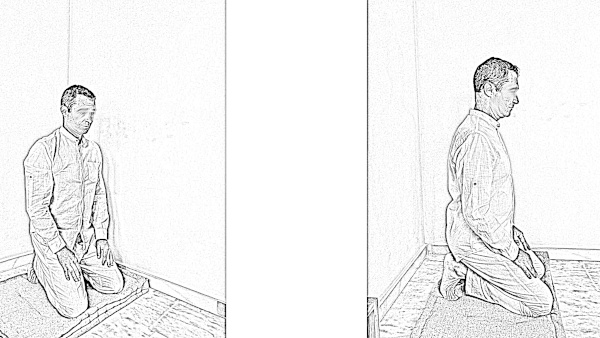
\includegraphics[scale=0.25,width=1\textwidth]{prep-man-ai.jpg}
		
	\end{minipage}
	\hfill
	\begin{minipage}{0.40\textwidth}
		\centering
		\caption{Las mujeres adoptan la misma postura, pero con el empeine de los pies hacia el suelo.}
		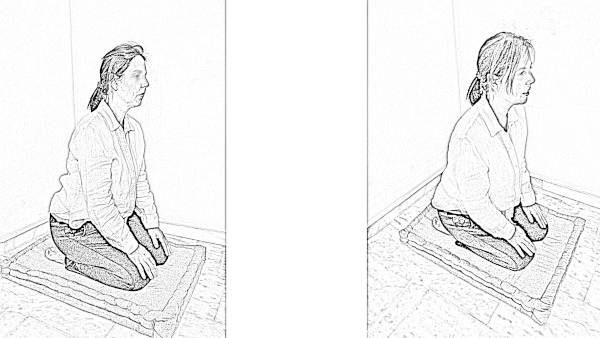
\includegraphics[scale=0.25,width=1\textwidth]{prep-woman-ai.jpg}
		
	\end{minipage}
	
\end{figure}


\subsection{El 'Añjali'}

Junte las palmas de las manos a la altura del pecho, apuntando hacia arriba en un ángulo de cuarenta y cinco grados con los dedos juntos.
\begin{figure}[h]
	\centering
	
	\begin{minipage}{0.40\textwidth}
		\centering
		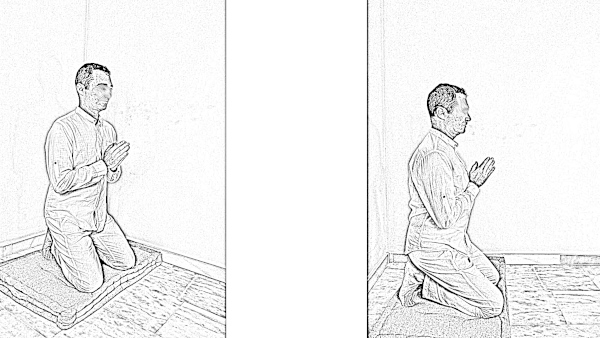
\includegraphics[scale=0.25,width=1\textwidth]{anjali-man-ai.jpg}
		%\label{fig:1}
	\end{minipage}
	\hfill
	\begin{minipage}{0.40\textwidth}
		\centering
		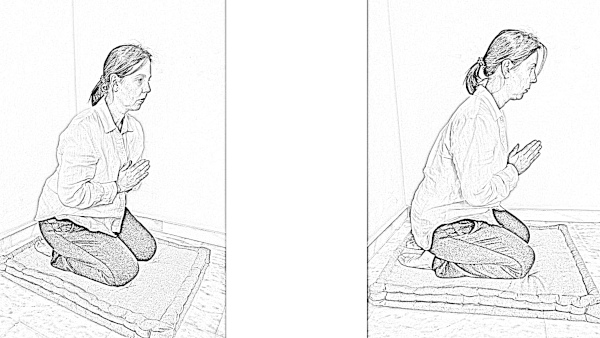
\includegraphics[scale=0.25,width=1\textwidth]{anjali-woman-ai.jpg}
		%\label{fig:2}
	\end{minipage}
	
\end{figure}

\subsection{El 'Vandana'}

Lleve el añjali (palmas juntas) hasta la frente de modo que los pulgares se coloquen entre las cejas y las puntas de los dedos índice estén en la línea del cabello.

\begin{figure}[h]
	\centering
	
	\begin{minipage}{0.40\textwidth}
		\centering
		\caption{Los hombres mantienen la cabeza recta.}
		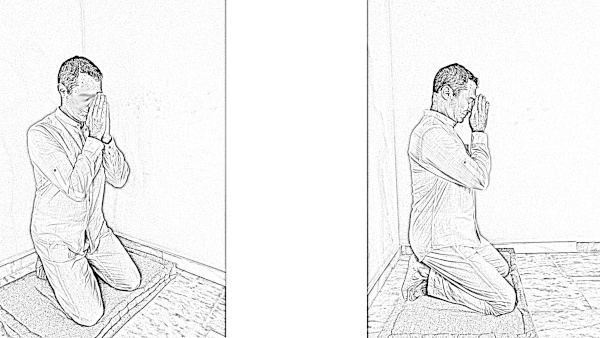
\includegraphics[scale=0.25,width=1\textwidth]{vandana-man-ai.jpg}
		%\label{fig:1}
	\end{minipage}
	\hfill
	\begin{minipage}{0.40\textwidth}
		\centering
		\caption{Las mujeres inclinan la cabeza ligeramente hacia adelante.}
		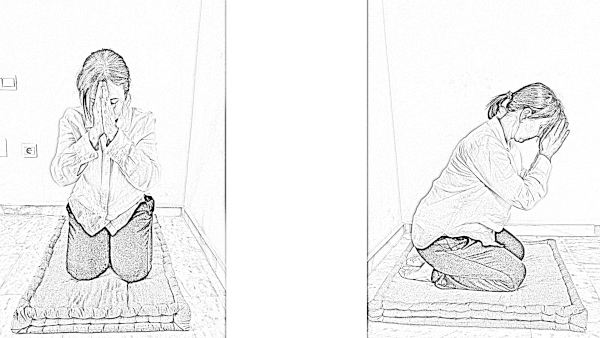
\includegraphics[scale=0.25,width=1\textwidth]{vandana-woman-ai.jpg}

		%\label{fig:2}
	\end{minipage}
\end{figure}
\enlargethispage{3\baselineskip}
\subsection{El 'Abhivada'}
Manteniendo la espalda recta, inclínese llevando la frente al suelo de modo que toque el espacio entre las palmas (aproximadamente a una distancia de un palmo), que ahora estarán boca abajo, planas sobre el suelo.
\begin{figure}[h]
	\centering
	\begin{minipage}{0.40\textwidth}
		\centering
		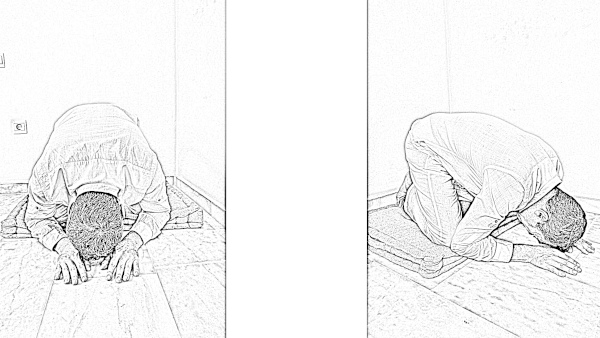
\includegraphics[scale=0.2,width=1\textwidth]{abhivada-man-ai.jpg}
		\caption{Los hombres mantienen los codos y las rodillas alineados y tocándose.}
		%\label{fig:1}
	\end{minipage}
	\hfill
	\begin{minipage}{0.40\textwidth}
		\centering
		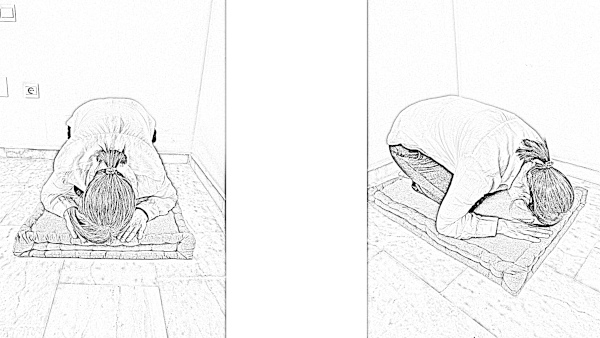
\includegraphics[scale=0.2,width=1\textwidth]{abhivada-woman-ai.jpg}
		\caption{Las mujeres colocan los codos a cada lado de las rodillas}
		%\label{fig:2}
	\end{minipage}
\end{figure}

\subsection{\thaiFont พับเพียบ ‘papiyap'}

\thaiFont{'พับเพียบ'} \normalfont(pronunciado 'papiyap') es un término tailandés que se refiere a la postura tradicional que se adopta al cantar. Sentarse ‘papiyap' significa sentarse con las piernas dobladas a un lado, como se muestra en el diagrama a continuación. La postura de piernas cruzadas o 'loto' se reserva para la práctica formal de meditación. Sentarse con las piernas o los pies apuntando hacia una imagen de Buddha o hacia los monásticos se considera irrespetuoso, ya que los pies son la parte más baja del cuerpo. Por lo tanto, ‘papiyap' es una postura apropiada para asumir mientras se canta. Sin embargo, cuando se cantan los versos de homenaje a la Triple Joya (Sección 1-Vol. 1), uno se arrodilla sobre sus talones. 
\enlargethispage{3\baselineskip}
\begin{figure}[h]
	\centering
	
	\begin{minipage}{0.40\textwidth}
		\centering
		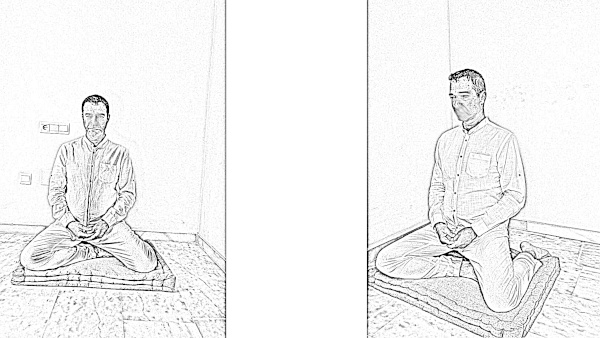
\includegraphics[scale=0.25,width=1\textwidth]{papiap-man-ai.jpg}
		\caption{Los hombres se sientan con una pierna doblada a un lado y la otra pierna cruzada frente a ellos, con la planta del pie tocando la rodilla.}
		%\label{fig:1}
	\end{minipage}
	\hfill
	\begin{minipage}{0.40\textwidth}
		\centering
		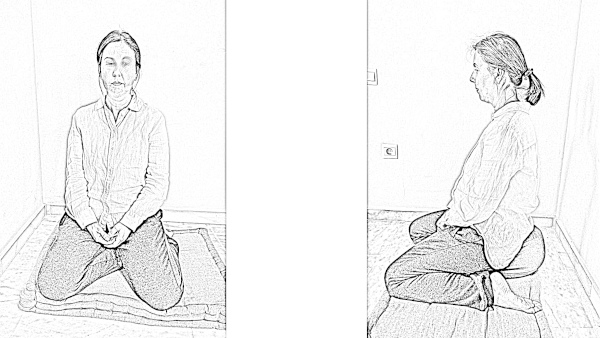
\includegraphics[scale=0.25,width=1\textwidth]{papiap-woman-ai.jpg}
		\caption{Las mujeres se sientan con una pierna doblada a un lado, pero con la otra pierna doblada debajo de ellas, manteniendo las rodillas juntas.}
		%\label{fig:2}
	\end{minipage}
	
\end{figure}

\subsection{Cambio de postura}


No está mal cambiar de postura cuando el dolor se agudiza, pero debe hacerse de manera educada. La mejor manera de cambiar de postura, ya sea sentado en meditación o mientras se canta, es cambiar la posición de las piernas desde atrás, inclinándose hacia adelante y usando una mano en el suelo para apoyarse.
\clearpage

\section{Etiqueta general en el monasterio y la sala de meditación}

El monasterio y, en particular, la sala principal de meditación son un espacio sagrado. La sala de meditación (sala Uposatha) debe proporcionar siempre, tanto a la comunidad monástica como a la laica, un entorno adecuado y propicio para la práctica de virtud, meditación y desarrollo de sabiduría. Hay ciertos tipos de comportamiento que contribuyen a una atmósfera de buena práctica espiritual y reflexión tranquila, y otros tipos de comportamiento que pueden destruirla rápidamente. Por lo tanto, es importante que cualquier persona que entre en el monasterio y, por extensión, en la sala de meditación, sea considerada respecto a cómo su comportamiento puede estar afectando a quienes le rodean. Esto beneficiará tanto a la propia práctica de Sati, como al entorno del monasterio en su conjunto.

Cuando entre en la sala principal, observe las siguientes prácticas:


\begin{enumerate}
\item Si es necesario hablar con alguien, es mejor salir a hacerlo. O al menos hágalo lo más silenciosa y brevemente posible, para no molestar a las personas a su alrededor que podrían estar tratando de meditar.

\item No se permiten sombreros, capuchas, gorros, zapatos, comida ni bebidas (incluidas botellas de agua) en la sala.

\item Se agradecería que los padres con bebés o niños pequeños sacaran a sus hijos de la sala si empiezan a llorar o a comportarse de forma incontrolable durante las sesiones de meditación y discursos de Dhamma.

\item Solo se pueden tomar fotos y vídeos con el permiso directo del monje de mayor antigüedad.

\item El monasterio es un lugar de celibato. La separación de sexos se practica estrictamente durante los retiros de meditación, y se debe evitar cualquier forma de contacto físico inadecuado con el sexo opuesto en cualquier lugar de los terrenos del monasterio.

\item Al entrar al monasterio, las personas deben evitar cualquier tipo de ropa que sea reveladora o inmodesta.

\item Por favor, no se siente apuntando con los pies hacia el altar ni hacia los monjes, ya que esto se considera una falta de respeto.

\item Por favor, no suba a la plataforma elevada frente al altar principal. Es un espacio reservado solo para la Saṅgha monástica.

\item Todos los teléfonos móviles o cualquier otro dispositivo eléctrico que pueda hacer ruido deben dejarse fuera de la sala o apagarse antes de entrar en ella.

\item Estas normas se aplican no solo a la sala principal de meditación, sino a cualquier edificio del monasterio donde se celebren discursos de Dhamma o se practique la meditación.
\end{enumerate}
Una actitud básica de moderación y respeto es todo lo que se necesita.

Gracias







\chapter{Glosario de términos en Pāli }

\enlargethispage{2\baselineskip}

\begin{description}

\item[Anatta] Literalmente, `no-alma,' i.e. impersonal, sin esencia individual;
 ni persona ni perteneciente a persona. Una de las tres características de todo fenómeno condicionado.

\item[Anicca] No permanente, inestable, de la naturaleza de aparecer y extinguirse. Una de las tres características de todo fenómeno condicionado.

\item[Arahaṁ/Arahant] Literalmente, ‘el que se lo merece’ --- un término aplicado a todos los seres iluminados. 

\item[Ariyapuggalā] ‘Seres Nobles’ o ‘Nobles Discípulos’ --- existen ocho tipos: aquellos que trabajan por alcanzar o aquellos que han alcanzado los cuatro diferentes niveles de la iluminación.

\item[Bhagavā] Epíteto reservado al Señor Buddha.

\item[Bhikkhu] Un monje budista que vive como monje mendicante, siguiendo 227 preceptos de entrenamiento que definen una vida de renuncia y simplicidad.

\item[Brahmā] Ser celestial; un dios en uno de los mas altos reinos espirituales.

\item[Buddha] 'El que despierta', uno que conoce las cosas como son; un potencial que existe en todo ser humano. El último Buddha conocido,
  Siddhattha Gotama, vivió y enseñó en la India en el 5th siglo a.C.

\item[Deva] Ser celestial. Menos refinado que brahmā; parecido al concepto de 'Ángel de la guarda'

\item[Dhamma] (Sánscrito: Dharma) Las enseñanzas de Buddha contenidas en las escrituras, no como dogma de fe, mas como una balsa o vehículo que lleva al discípulo hasta la liberación. Cuando se escribe como ‘\emph{dhamma}’, i.e.
  con `d' minúscula, se refiere a 'cosa’ o 'elemento'.

\item[Dukkha] Literalmente, ‘difícil de soportar’ --- mal-estar, inquietud mental, angustia, insatisfacción, des-contento, estrés, sufrimiento. Una de las tres características de los fenómenos condicionados.


\item[Vida Santa (brahmacariya)] Literalmente: la conducta de Brahma; usualmente referido a la vida monástica. Usar este término implica voto de celibato.

\item[Jhāna] Absorción mental. Estado de gran concentración enfocado en una simple sensación o noción mental.

\item[Kamma] (Sánscrito: karma) Acción; acciones creadas por impulso habitual, con intención.

\item[Khandhā] Los cinco agregados que componen un ser, tanto fisicos como mentales ---
  estos son: \emph{rūpa, vedanā, saññā, saṅkhārā, viññāṇa.} Apego a cualquier de estos como, ‘Esto es mio’, ‘Yo soy esto’ o, ‘Esto es mi alma’ es
  \emph{upādāna} --- apego.

\item[Māra] Personificación de las fuerzas del mal. Durante la lucha de Buddha por la iluminación, Māra se manifestó tratando de desviarle de su meta.

\item[Nibbāna] (Sánscrito: Nirvāṇa) Literalmente, ‘frescor’ --- el estado de liberación de todo sufrimiento e impurezas, la meta del camino budista.

\item[Paccekabuddha] Buddha solitario --- alguien que se ilumina por sus propios medios sin depender de maestro alguno, pero que (a diferencia de Buddha) no posee discípulos.

\item[Paritta] Versos cantados particularmente para bendiciones y protección.

\item[Parinibbāna] El perecimiento definitivo de Buddha, i.e. entrada definitiva en 
  Nibbāna.

\item[Puñña] Mérito, acumulación de buena fortuna, bendiciones o bienestar resultante de la práctica del Dhamma.

\item[Rūpa] Forma o materia. Los elementos físicos que componen el cuerpo,
  i.e. tierra, agua, fuego y aire (solidez, cohesión, temperatura y
  vibración).

\item[Saṅgha] La comunidad de aquellos que practican el camino de Buddha.
  Más específicamente, aquellos que se comprometen formalmente al estilo de vida de monjes mendicantes.

\item[Saṅkhārā] Formaciones, construcciones, todas las cosas condicionadas, o impulsos voluntarios, es decir, todos los estados mentales con excepción de Vedana y Sañña, que le dan matiz a los pensamientos volviéndolos en 'buenos', 'malos' o 'neutros'.

\item[Saññā] Percepción, la función mental de reconocer. Impone valores a las cosas dependiendo de experiencias previas.

\item[Sati] Este término proviene del verbo sarati que significa 'recordar'. Recordar el qué? Recordar el objeto de meditación. 

\item[Tathāgata] ‘Así ido’ o ‘Así venido’ --- dando el sentido de 'el que viene de vuelta de todo' uno que ha ido más allá del sufrimiento y la muerte; uno que experimenta las cosas como realmente son, sin ilusión. El epíteto que Buddha se aplicó a sí mismo después de obtener la Iluminación perfecta.

\item[Joya Triple] Buddha, Dhamma y Saṅgha.

\item[Vedanā] Sensación --- Sensaciones mentales o físicas ya sean agradables, desagradables o neutras.

\item[Viññāṇa] Conciencia sensorial --- proceso por el cual puedo existir la visión, oir, oler, gustar, tocar y pensar.

\end{description}


%
\cleartorecto

\thispagestyle{empty}

\newlength\ackWidth
\ifaivedition
\setlength{\ackWidth}{0.77\linewidth}
\else
\setlength{\ackWidth}{0.8\linewidth}
\fi

{\centering

\ifaivedition
\vspace*{9\baselineskip}
\else
\vspace*{6\baselineskip}
\fi

\begin{minipage}{\ackWidth}
\setlength{\parskip}{8pt}

{\instructionFont\color{instruction}Cuidado de los libros de Dhamma:}

\bigskip

Los libros de Dhamma contienen las enseñanzas de Buddha y señalan el camino hacia la liberación de saṁsara. Por lo tanto, deben tratarse con respeto: deben mantenerse fuera del suelo y de lugares donde la gente se sienta o camina, y no deben pasarse por encima. Deben cubrirse o protegerse para su transporte y guardarse en un lugar alto y limpio, separado de materiales más ‘mundanos’. No se deben colocar otros objetos encima de los libros y materiales de Dhamma. Humedecerse los dedos para pasar las páginas se considera de mala educación. Si es necesario deshacerse de materiales de Dhamma, en lugar de tirarlos a la basura, deben quemarse, con sati y una actitud reverencial.

\end{minipage}

}



\clearpage

\thispagestyle{plain}

{\small
\setlength{\parindent}{0pt}%
\raggedright\label{copyright-details}
\setlength{\parskip}{10pt}
{\centering

{\LARGE\ccbyncnd}

Este trabajo está licenciado con una Licencia Creative Commons\\
Atribución-NoComercial-SinDerivadas 4.0 Internacional.\\
\url{http://creativecommons.org/licenses/by-nc-nd/4.0/deed.pt}

}

Usted es libre de:

\begin{packeditemize}
\item Compartir — copiar y redistribuir el material en cualquier medio o formato
\end{packeditemize}

La licenciante no puede revocar estas libertades en tanto usted siga los términos de la licencia.

Bajo los siguientes términos:

\begin{packeditemize}
\item Atribución — Usted debe dar crédito de manera adecuada, brindar un enlace a la licencia, e indicar si se han realizado cambios. Puede hacerlo en cualquier forma razonable, pero no de forma tal que sugiera que usted o su uso tienen el apoyo de la licenciante.
\item NoComercial — Usted no puede hacer uso del material con propósitos comerciales.
\item SinDerivadas — Si remezcla, transforma o crea a partir del material, no podrá distribuir el material modificado.
\end{packeditemize}

No hay restricciones adicionales — No puede aplicar términos legales ni medidas tecnológicas que restrinjan legalmente a otras a hacer cualquier uso permitido por la licencia.

Avisos:

No tiene que cumplir con la licencia para elementos del materiale en el dominio público o cuando su uso esté permitido por una excepción o limitación aplicable.

No se dan garantías. La licencia podría no darle todos los permisos que necesita para el uso que tenga previsto. Por ejemplo, otros derechos como publicidad, privacidad, o derechos morales pueden limitar la forma en que utilice el material.

Publicações Sumedhārāma es parte de ``Budismo Theravada da Floresta -- Comunidade Religiosa'', una ``Pessoa Colectiva Religiosa'' registrada en Portugal con el NIPC 592010040.

``Budismo Theravada da Floresta -- Comunidade Religiosa'', actuando como Publicações Sumedhārāma, reclama el direcho moral de ser identificado como autor de este libro.

``Budismo Theravada da Floresta -- Comunidade Religiosa'', requiere que sea atribuida la autoría de este trabajo a Publicações Sumedhārāma siempre que sea reproducido, distribuido, presentado o representado.

}


\emptyUntilEven

\end{document}
